\documentclass[twoside]{book}

% Packages required by doxygen
\usepackage{calc}
\usepackage{doxygen}
\usepackage{graphicx}
\usepackage[utf8]{inputenc}
\usepackage{makeidx}
\usepackage{multicol}
\usepackage{multirow}
\usepackage{textcomp}
\usepackage[table]{xcolor}

% Font selection
\usepackage[T1]{fontenc}
\usepackage{mathptmx}
\usepackage[scaled=.90]{helvet}
\usepackage{courier}
\usepackage{amssymb}
\usepackage{sectsty}
\renewcommand{\familydefault}{\sfdefault}
\allsectionsfont{%
  \fontseries{bc}\selectfont%
  \color{darkgray}%
}
\renewcommand{\DoxyLabelFont}{%
  \fontseries{bc}\selectfont%
  \color{darkgray}%
}

% Page & text layout
\usepackage{geometry}
\geometry{%
  a4paper,%
  top=2.5cm,%
  bottom=2.5cm,%
  left=2.5cm,%
  right=2.5cm%
}
\tolerance=750
\hfuzz=15pt
\hbadness=750
\setlength{\emergencystretch}{15pt}
\setlength{\parindent}{0cm}
\setlength{\parskip}{0.2cm}
\makeatletter
\renewcommand{\paragraph}{%
  \@startsection{paragraph}{4}{0ex}{-1.0ex}{1.0ex}{%
    \normalfont\normalsize\bfseries\SS@parafont%
  }%
}
\renewcommand{\subparagraph}{%
  \@startsection{subparagraph}{5}{0ex}{-1.0ex}{1.0ex}{%
    \normalfont\normalsize\bfseries\SS@subparafont%
  }%
}
\makeatother

% Headers & footers
\usepackage{fancyhdr}
\pagestyle{fancyplain}
\fancyhead[LE]{\fancyplain{}{\bfseries\thepage}}
\fancyhead[CE]{\fancyplain{}{}}
\fancyhead[RE]{\fancyplain{}{\bfseries\leftmark}}
\fancyhead[LO]{\fancyplain{}{\bfseries\rightmark}}
\fancyhead[CO]{\fancyplain{}{}}
\fancyhead[RO]{\fancyplain{}{\bfseries\thepage}}
\fancyfoot[LE]{\fancyplain{}{}}
\fancyfoot[CE]{\fancyplain{}{}}
\fancyfoot[RE]{\fancyplain{}{\bfseries\scriptsize Generated on Wed Aug 15 2018 03\-:50\-:10 for Electron\-Neutrino\-Selection by Doxygen }}
\fancyfoot[LO]{\fancyplain{}{\bfseries\scriptsize Generated on Wed Aug 15 2018 03\-:50\-:10 for Electron\-Neutrino\-Selection by Doxygen }}
\fancyfoot[CO]{\fancyplain{}{}}
\fancyfoot[RO]{\fancyplain{}{}}
\renewcommand{\footrulewidth}{0.4pt}
\renewcommand{\chaptermark}[1]{%
  \markboth{#1}{}%
}
\renewcommand{\sectionmark}[1]{%
  \markright{\thesection\ #1}%
}

% Indices & bibliography
\usepackage{natbib}
\usepackage[titles]{tocloft}
\setcounter{tocdepth}{3}
\setcounter{secnumdepth}{5}
\makeindex

% Hyperlinks (required, but should be loaded last)
\usepackage{ifpdf}
\ifpdf
  \usepackage[pdftex,pagebackref=true]{hyperref}
\else
  \usepackage[ps2pdf,pagebackref=true]{hyperref}
\fi
\hypersetup{%
  colorlinks=true,%
  linkcolor=blue,%
  citecolor=blue,%
  unicode%
}

% Custom commands
\newcommand{\clearemptydoublepage}{%
  \newpage{\pagestyle{empty}\cleardoublepage}%
}


%===== C O N T E N T S =====

\begin{document}

% Titlepage & ToC
\hypersetup{pageanchor=false}
\pagenumbering{roman}
\begin{titlepage}
\vspace*{7cm}
\begin{center}%
{\Large Electron\-Neutrino\-Selection }\\
\vspace*{1cm}
{\large Generated by Doxygen 1.8.6}\\
\vspace*{0.5cm}
{\small Wed Aug 15 2018 03:50:10}\\
\end{center}
\end{titlepage}
\clearemptydoublepage
\tableofcontents
\clearemptydoublepage
\pagenumbering{arabic}
\hypersetup{pageanchor=true}

%--- Begin generated contents ---
\chapter{Module Index}
\section{Modules}
Here is a list of all modules\-:\begin{DoxyCompactList}
\item \contentsline{section}{Lee}{\pageref{group__lee}}{}
\end{DoxyCompactList}

\chapter{Hierarchical Index}
\section{Class Hierarchy}
This inheritance list is sorted roughly, but not completely, alphabetically\-:\begin{DoxyCompactList}
\item E\-D\-Analyzer\begin{DoxyCompactList}
\item \contentsline{section}{lee\-:\-:Pandora\-L\-E\-E\-Analyzer}{\pageref{classlee_1_1PandoraLEEAnalyzer}}{}
\end{DoxyCompactList}
\item E\-D\-Filter\begin{DoxyCompactList}
\item \contentsline{section}{lee\-:\-:Electron\-Neutrino\-Filter}{\pageref{classlee_1_1ElectronNeutrinoFilter}}{}
\end{DoxyCompactList}
\item \contentsline{section}{Electron\-Event\-Selection\-Alg}{\pageref{classElectronEventSelectionAlg}}{}
\item \contentsline{section}{lee\-:\-:Electron\-Event\-Selection\-Alg}{\pageref{classlee_1_1ElectronEventSelectionAlg}}{}
\item \contentsline{section}{Energy\-Helper}{\pageref{classEnergyHelper}}{}
\item \contentsline{section}{Geometry\-Helper}{\pageref{classGeometryHelper}}{}
\item \contentsline{section}{lee\-:\-:Helper\-Base}{\pageref{classlee_1_1HelperBase}}{}
\begin{DoxyCompactList}
\item \contentsline{section}{lee\-:\-:Energy\-Helper}{\pageref{classlee_1_1EnergyHelper}}{}
\item \contentsline{section}{lee\-:\-:Geometry\-Helper}{\pageref{classlee_1_1GeometryHelper}}{}
\item \contentsline{section}{lee\-:\-:Pandora\-Interface\-Helper}{\pageref{classlee_1_1PandoraInterfaceHelper}}{}
\end{DoxyCompactList}
\item \contentsline{section}{Pandora\-Interface\-Helper}{\pageref{classPandoraInterfaceHelper}}{}
\item \contentsline{section}{Pandora\-L\-E\-E\-Analyzer}{\pageref{classPandoraLEEAnalyzer}}{}
\end{DoxyCompactList}

\chapter{Class Index}
\section{Class List}
Here are the classes, structs, unions and interfaces with brief descriptions\-:\begin{DoxyCompactList}
\item\contentsline{section}{\hyperlink{classElectronEventSelectionAlg}{Electron\-Event\-Selection\-Alg} \\*Class that performs the selection algorithms, requiring a certain topology and a flash matched with the neutrino candidate }{\pageref{classElectronEventSelectionAlg}}{}
\item\contentsline{section}{\hyperlink{classlee_1_1ElectronEventSelectionAlg}{lee\-::\-Electron\-Event\-Selection\-Alg} }{\pageref{classlee_1_1ElectronEventSelectionAlg}}{}
\item\contentsline{section}{\hyperlink{classlee_1_1ElectronNeutrinoFilter}{lee\-::\-Electron\-Neutrino\-Filter} }{\pageref{classlee_1_1ElectronNeutrinoFilter}}{}
\item\contentsline{section}{\hyperlink{classEnergyHelper}{Energy\-Helper} \\*Helper class with methods accessing calorimetric information (energy and d\-E/dx) }{\pageref{classEnergyHelper}}{}
\item\contentsline{section}{\hyperlink{classlee_1_1EnergyHelper}{lee\-::\-Energy\-Helper} }{\pageref{classlee_1_1EnergyHelper}}{}
\item\contentsline{section}{\hyperlink{classlee_1_1GeometryHelper}{lee\-::\-Geometry\-Helper} }{\pageref{classlee_1_1GeometryHelper}}{}
\item\contentsline{section}{\hyperlink{classGeometryHelper}{Geometry\-Helper} \\*Helper class with geometric methods (distance, point in a plane, etc. ) }{\pageref{classGeometryHelper}}{}
\item\contentsline{section}{\hyperlink{classlee_1_1HelperBase}{lee\-::\-Helper\-Base} }{\pageref{classlee_1_1HelperBase}}{}
\item\contentsline{section}{\hyperlink{classPandoraInterfaceHelper}{Pandora\-Interface\-Helper} \\*Helper class with methods useful to interface with Pandora information. It contains the methods use to perform reco/true matching }{\pageref{classPandoraInterfaceHelper}}{}
\item\contentsline{section}{\hyperlink{classlee_1_1PandoraInterfaceHelper}{lee\-::\-Pandora\-Interface\-Helper} }{\pageref{classlee_1_1PandoraInterfaceHelper}}{}
\item\contentsline{section}{\hyperlink{classlee_1_1PandoraLEEAnalyzer}{lee\-::\-Pandora\-L\-E\-E\-Analyzer} }{\pageref{classlee_1_1PandoraLEEAnalyzer}}{}
\item\contentsline{section}{\hyperlink{classPandoraLEEAnalyzer}{Pandora\-L\-E\-E\-Analyzer} \\*Main analyzer class filling a R\-O\-O\-T T\-Tree with information from the selected electron neutrino candidate }{\pageref{classPandoraLEEAnalyzer}}{}
\end{DoxyCompactList}

\chapter{Module Documentation}
\hypertarget{group__lee}{\section{Lee}
\label{group__lee}\index{Lee@{Lee}}
}
\subsection*{Classes}
\begin{DoxyCompactItemize}
\item 
class \hyperlink{classlee_1_1ElectronEventSelectionAlg}{lee\-::\-Electron\-Event\-Selection\-Alg}
\item 
class \hyperlink{classlee_1_1EnergyHelper}{lee\-::\-Energy\-Helper}
\item 
class \hyperlink{classlee_1_1GeometryHelper}{lee\-::\-Geometry\-Helper}
\item 
class \hyperlink{classlee_1_1PandoraInterfaceHelper}{lee\-::\-Pandora\-Interface\-Helper}
\item 
class \hyperlink{classlee_1_1PandoraLEEAnalyzer}{lee\-::\-Pandora\-L\-E\-E\-Analyzer}
\end{DoxyCompactItemize}
\subsection*{Typedefs}
\begin{DoxyCompactItemize}
\item 
\hypertarget{group__lee_ga70b6dfa1b2176c8ecbee29c567946890}{typedef std\-::map$<$ art\-::\-Ptr\\*
$<$ recob\-::\-P\-F\-Particle $>$\\*
, art\-::\-Ptr$<$ simb\-::\-M\-C\-Particle $>$ $>$ {\bfseries lar\-\_\-pandora\-::\-P\-F\-Particles\-To\-M\-C\-Particles}}\label{group__lee_ga70b6dfa1b2176c8ecbee29c567946890}

\item 
\hypertarget{group__lee_ga1e4126ea41de810a723eb4c1023fb418}{typedef std\-::map$<$ art\-::\-Ptr\\*
$<$ recob\-::\-P\-F\-Particle $>$\\*
, unsigned int $>$ {\bfseries lee\-::\-Reco\-Particle\-To\-N\-Matched\-Hits}}\label{group__lee_ga1e4126ea41de810a723eb4c1023fb418}

\item 
\hypertarget{group__lee_gad68c1843c146182933b27bf7be0455a4}{typedef std\-::map$<$ art\-::\-Ptr\\*
$<$ simb\-::\-M\-C\-Particle $>$\\*
, Reco\-Particle\-To\-N\-Matched\-Hits $>$ {\bfseries lee\-::\-Particle\-Matching\-Map}}\label{group__lee_gad68c1843c146182933b27bf7be0455a4}

\item 
\hypertarget{group__lee_ga084ff379386cea31dbc631216b56b9eb}{typedef std\-::set$<$ art\-::\-Ptr\\*
$<$ recob\-::\-P\-F\-Particle $>$ $>$ {\bfseries lee\-::\-P\-F\-Particle\-Set}}\label{group__lee_ga084ff379386cea31dbc631216b56b9eb}

\item 
\hypertarget{group__lee_gab1ec016bd8fc6df09c6f95dba3962bba}{typedef std\-::set$<$ art\-::\-Ptr\\*
$<$ simb\-::\-M\-C\-Particle $>$ $>$ {\bfseries lee\-::\-M\-C\-Particle\-Set}}\label{group__lee_gab1ec016bd8fc6df09c6f95dba3962bba}

\end{DoxyCompactItemize}
\subsection*{Functions}
\begin{DoxyCompactItemize}
\item 
bool \hyperlink{group__lee_ga59666f2bec60817a81fcdd467d9b9641}{lee\-::\-Electron\-Event\-Selection\-Alg\-::event\-Selected} (const art\-::\-Event \&evt)
\begin{DoxyCompactList}\small\item\em Main Event Selection Function. \end{DoxyCompactList}\item 
void \hyperlink{group__lee_ga8f1378ec08aba381d438816c8bc31951}{lee\-::\-Electron\-Event\-Selection\-Alg\-::reconfigure} (fhicl\-::\-Parameter\-Set const \&p)
\begin{DoxyCompactList}\small\item\em Configure all of the parameters of this class. \end{DoxyCompactList}\item 
const std\-::map$<$ size\-\_\-t, int $>$ \hyperlink{group__lee_ga1853e2053d74627cd4466cf670dc0c31}{lee\-::\-Electron\-Event\-Selection\-Alg\-::opticalfilter} (const art\-::\-Event \&evt, const std\-::vector$<$ size\-\_\-t $>$ \&pfplist, const art\-::\-Valid\-Handle$<$ std\-::vector$<$ recob\-::\-P\-F\-Particle $>$$>$ pfparticle\-\_\-handle)
\begin{DoxyCompactList}\small\item\em Checks if there is a flash within the 3.\-2-\/4.\-8 ms window and compatible with the center of charge. \end{DoxyCompactList}\item 
const std\-::map$<$ size\-\_\-t, int $>$ \hyperlink{group__lee_ga4d8d979b26116ec25d26884702d0f9c6}{lee\-::\-Electron\-Event\-Selection\-Alg\-::flash\-Based\-Selection} (const art\-::\-Event \&evt, const std\-::vector$<$ size\-\_\-t $>$ \&pfplist, const art\-::\-Valid\-Handle$<$ std\-::vector$<$ recob\-::\-P\-F\-Particle $>$$>$ pfparticle\-\_\-handle)
\begin{DoxyCompactList}\small\item\em Checks if there is a flash within the flash\-\_\-window\-\_\-start -\/ flash\-\_\-window\-\_\-end window with enough P\-E. and compatible with the center of charge, the best one is selected using flashmatching. \end{DoxyCompactList}\item 
const flashana\-::\-Q\-Cluster\-\_\-t \hyperlink{group__lee_ga06a3e470d9b2ca729d25822fac19e455}{lee\-::\-Electron\-Event\-Selection\-Alg\-::collect3\-D\-Hits} (const art\-::\-Event \&evt, const std\-::vector$<$ size\-\_\-t $>$ \&pfplist)
\begin{DoxyCompactList}\small\item\em Creates a photon cluster for a neutrino pfp hierarchy P\-F\-Particle. \end{DoxyCompactList}\item 
T\-Vector3 \hyperlink{group__lee_gafb99143e1546158d3f030724694e6a51}{lee\-::\-Electron\-Event\-Selection\-Alg\-::space\-Charge\-True\-To\-Reco} (const T\-Vector3 \&xyz)
\begin{DoxyCompactList}\small\item\em Return the true coordinates corrected by the space-\/charge effect. \end{DoxyCompactList}\item 
\hypertarget{group__lee_gad936812d5e9dc7999a37c75b84b04ada}{void \hyperlink{group__lee_gad936812d5e9dc7999a37c75b84b04ada}{lee\-::\-Electron\-Event\-Selection\-Alg\-::clear} ()}\label{group__lee_gad936812d5e9dc7999a37c75b84b04ada}

\begin{DoxyCompactList}\small\item\em Reset internal variables. \end{DoxyCompactList}\item 
\hypertarget{group__lee_ga317c107f710fc965cd7e062ac933d3df}{const std\-::vector$<$ size\-\_\-t $>$ \& \hyperlink{group__lee_ga317c107f710fc965cd7e062ac933d3df}{lee\-::\-Electron\-Event\-Selection\-Alg\-::get\-\_\-primary\-\_\-indexes} () const }\label{group__lee_ga317c107f710fc965cd7e062ac933d3df}

\begin{DoxyCompactList}\small\item\em Return a list of the selected pfparticle top level neutrino candidate indexes. \end{DoxyCompactList}\item 
\hypertarget{group__lee_ga6259851e755db48eb0dd831708212e27}{const size\-\_\-t \& \hyperlink{group__lee_ga6259851e755db48eb0dd831708212e27}{lee\-::\-Electron\-Event\-Selection\-Alg\-::get\-\_\-n\-\_\-neutrino\-\_\-candidates} () const }\label{group__lee_ga6259851e755db48eb0dd831708212e27}

\begin{DoxyCompactList}\small\item\em Return the number of neutrino candidates. \end{DoxyCompactList}\item 
const std\-::map$<$ size\-\_\-t, bool $>$ \& \hyperlink{group__lee_gab34dc2b97e0065b07a5233e3b46b83a4}{lee\-::\-Electron\-Event\-Selection\-Alg\-::get\-\_\-neutrino\-\_\-candidate\-\_\-passed} () const 
\begin{DoxyCompactList}\small\item\em Inform whether a particular candidate passed or failed the algorithm. \end{DoxyCompactList}\item 
\hypertarget{group__lee_gaffda5b411008752c1355a9dd3a1d9c1e}{const std\-::map$<$ size\-\_\-t, int $>$ \& \hyperlink{group__lee_gaffda5b411008752c1355a9dd3a1d9c1e}{lee\-::\-Electron\-Event\-Selection\-Alg\-::get\-\_\-op\-\_\-flash\-\_\-indexes} () const }\label{group__lee_gaffda5b411008752c1355a9dd3a1d9c1e}

\begin{DoxyCompactList}\small\item\em Return the index of the flash matched with the pfparticle. \end{DoxyCompactList}\item 
\hypertarget{group__lee_gac098d39d04f407c9bfc574da4b82fee6}{const std\-::map$<$ size\-\_\-t, \\*
T\-Vector3 $>$ \& \hyperlink{group__lee_gac098d39d04f407c9bfc574da4b82fee6}{lee\-::\-Electron\-Event\-Selection\-Alg\-::get\-\_\-neutrino\-\_\-vertex} () const }\label{group__lee_gac098d39d04f407c9bfc574da4b82fee6}

\begin{DoxyCompactList}\small\item\em Return the pandora calculated vertex indexed by pfparticle id number. \end{DoxyCompactList}\item 
\hypertarget{group__lee_ga43afa7fb8c10333f89774c6d4ea714dc}{const std\-::map$<$ size\-\_\-t, int $>$ \& \hyperlink{group__lee_ga43afa7fb8c10333f89774c6d4ea714dc}{lee\-::\-Electron\-Event\-Selection\-Alg\-::get\-\_\-n\-\_\-showers} () const }\label{group__lee_ga43afa7fb8c10333f89774c6d4ea714dc}

\begin{DoxyCompactList}\small\item\em Return number of showers for this pfparticle. \end{DoxyCompactList}\item 
\hypertarget{group__lee_gad24d64eca5e56d0550572b24d5e213f7}{const std\-::map$<$ size\-\_\-t, int $>$ \& \hyperlink{group__lee_gad24d64eca5e56d0550572b24d5e213f7}{lee\-::\-Electron\-Event\-Selection\-Alg\-::get\-\_\-n\-\_\-tracks} () const }\label{group__lee_gad24d64eca5e56d0550572b24d5e213f7}

\begin{DoxyCompactList}\small\item\em Return number of tracks for pfparticle index. \end{DoxyCompactList}\item 
\hypertarget{group__lee_ga7ea645ce175506b368ceb116bbb77889}{const std\-::map$<$ size\-\_\-t, \\*
std\-::vector$<$ size\-\_\-t $>$ $>$ \& \hyperlink{group__lee_ga7ea645ce175506b368ceb116bbb77889}{lee\-::\-Electron\-Event\-Selection\-Alg\-::get\-\_\-pfp\-\_\-id\-\_\-showers\-\_\-from\-\_\-primary} () const }\label{group__lee_ga7ea645ce175506b368ceb116bbb77889}

\begin{DoxyCompactList}\small\item\em Return the list of pfparticle indexes that are showers that are associated with primary pfparticle indexes. \end{DoxyCompactList}\item 
\hypertarget{group__lee_ga00266c70e046a9ee27e979be75925a09}{const std\-::map$<$ size\-\_\-t, \\*
std\-::vector$<$ size\-\_\-t $>$ $>$ \& \hyperlink{group__lee_ga00266c70e046a9ee27e979be75925a09}{lee\-::\-Electron\-Event\-Selection\-Alg\-::get\-\_\-pfp\-\_\-id\-\_\-tracks\-\_\-from\-\_\-primary} () const }\label{group__lee_ga00266c70e046a9ee27e979be75925a09}

\begin{DoxyCompactList}\small\item\em Return the list of pfparticle indexes that are tracks that are associated with primary pfparticle indexes. \end{DoxyCompactList}\item 
\hypertarget{group__lee_ga306e62904f73e727c6f938d2a197f68e}{const std\-::vector$<$ double $>$ \& \hyperlink{group__lee_ga306e62904f73e727c6f938d2a197f68e}{lee\-::\-Electron\-Event\-Selection\-Alg\-::get\-\_\-flash\-\_\-\-P\-E} () const }\label{group__lee_ga306e62904f73e727c6f938d2a197f68e}

\begin{DoxyCompactList}\small\item\em Return the list of total P\-E of the flashes. \end{DoxyCompactList}\item 
\hypertarget{group__lee_ga9990f4a980662e786fc8e38146ce4456}{const std\-::vector$<$ double $>$ \& \hyperlink{group__lee_ga9990f4a980662e786fc8e38146ce4456}{lee\-::\-Electron\-Event\-Selection\-Alg\-::get\-\_\-flash\-\_\-time} () const }\label{group__lee_ga9990f4a980662e786fc8e38146ce4456}

\begin{DoxyCompactList}\small\item\em Return the list of times of the flashes. \end{DoxyCompactList}\item 
\hypertarget{group__lee_ga69b697a2eec43de221621bd4aca906e2}{const double \& \hyperlink{group__lee_ga69b697a2eec43de221621bd4aca906e2}{lee\-::\-Electron\-Event\-Selection\-Alg\-::get\-\_\-flash\-\_\-x} () const }\label{group__lee_ga69b697a2eec43de221621bd4aca906e2}

\begin{DoxyCompactList}\small\item\em Return the position in x of the flash. \end{DoxyCompactList}\item 
\hypertarget{group__lee_ga2c653a5d3225c3e3aa5dc84738ffa086}{const double \& \hyperlink{group__lee_ga2c653a5d3225c3e3aa5dc84738ffa086}{lee\-::\-Electron\-Event\-Selection\-Alg\-::get\-\_\-\-T\-P\-C\-\_\-x} () const }\label{group__lee_ga2c653a5d3225c3e3aa5dc84738ffa086}

\begin{DoxyCompactList}\small\item\em Return the position in x of the center of the collected charge. \end{DoxyCompactList}\item 
void \hyperlink{group__lee_ga4523185d78d6b7aa94dbf26475750282}{lee\-::\-Energy\-Helper\-::reconfigure} (fhicl\-::\-Parameter\-Set const \&pset)
\begin{DoxyCompactList}\small\item\em Configure all of the parameters of this class. \end{DoxyCompactList}\item 
void \hyperlink{group__lee_ga2da6cbede1c42495e837b3a8b733be48}{lee\-::\-Energy\-Helper\-::d\-Qdx} (const recob\-::\-Shower $\ast$shower\-\_\-obj, std\-::vector$<$ art\-::\-Ptr$<$ recob\-::\-Cluster $>$$>$ $\ast$clusters, art\-::\-Find\-Many\-P$<$ recob\-::\-Hit $>$ $\ast$hits\-\_\-per\-\_\-cluster, std\-::vector$<$ double $>$ \&dqdx, std\-::vector$<$ double $>$ \&dqdx\-\_\-hits, std\-::vector$<$ double $>$ \&pitches, std\-::vector$<$ int $>$ \&dqdx\-\_\-hits\-\_\-in\-\_\-the\-\_\-box)
\begin{DoxyCompactList}\small\item\em Measure the d\-Qdx of a shower. \end{DoxyCompactList}\item 
double \hyperlink{group__lee_ga493326200e39f3aaa22999c55c22b6f5}{lee\-::\-Energy\-Helper\-::\-P\-I\-D} (const std\-::vector$<$ art\-::\-Ptr$<$ anab\-::\-Particle\-I\-D $>$$>$ $\ast$pids, int track\-I\-D, std\-::string Alg\-Name, anab\-::k\-Variable\-Type Variable\-Type, int pdg\-Code)
\begin{DoxyCompactList}\small\item\em Return the value of a specific Particle\-I\-D algorithm for a single track. \end{DoxyCompactList}\item 
void \hyperlink{group__lee_ga2844c7f27f79fbe5e16d9c674ca4afa1}{lee\-::\-Energy\-Helper\-::d\-Edx\-\_\-from\-\_\-d\-Qdx} (std\-::vector$<$ double $>$ \&dedx, std\-::vector$<$ double $>$ dqdx)
\begin{DoxyCompactList}\small\item\em Convert d\-Q/dx vector into d\-E/dx vector (in Me\-V) \end{DoxyCompactList}\item 
void \hyperlink{group__lee_gac5f41d2b1bee9a0f761179f3059f8a49}{lee\-::\-Energy\-Helper\-::\-P\-C\-A} (std\-::vector$<$ art\-::\-Ptr$<$ recob\-::\-Cluster $>$$>$ $\ast$clusters, art\-::\-Find\-Many\-P$<$ recob\-::\-Hit $>$ $\ast$hits\-\_\-per\-\_\-cluster, std\-::vector$<$ std\-::vector$<$ double $>$$>$ \&pca\-\_\-planes)
\begin{DoxyCompactList}\small\item\em Principal Component Analysis of reconstructed clusters. \end{DoxyCompactList}\item 
void \hyperlink{group__lee_gaf141846d9be1716bcfcf351633bdf8e7}{lee\-::\-Energy\-Helper\-::get\-\_\-cali} (std\-::vector$<$ art\-::\-Ptr$<$ recob\-::\-Space\-Point $>$$>$ $\ast$spcpnts, art\-::\-Find\-Many\-P$<$ recob\-::\-Hit $>$ $\ast$hits\-\_\-per\-\_\-spcpnts, std\-::vector$<$ double $>$ \&cali\-\_\-corr)
\begin{DoxyCompactList}\small\item\em Calibration value for the energy of a reconstructed object. \end{DoxyCompactList}\item 
void \hyperlink{group__lee_gaabbb21a3db419c9580aec4976c5137a9}{lee\-::\-Energy\-Helper\-::energy\-\_\-from\-\_\-hits} (std\-::vector$<$ art\-::\-Ptr$<$ recob\-::\-Cluster $>$$>$ $\ast$clusters, art\-::\-Find\-Many\-P$<$ recob\-::\-Hit $>$ $\ast$hits\-\_\-per\-\_\-cluster, std\-::vector$<$ int $>$ \&n\-Hits, std\-::vector$<$ double $>$ \&pfenergy)
\begin{DoxyCompactList}\small\item\em Measure calorimetric energy for a reconstructed object. \end{DoxyCompactList}\item 
void \hyperlink{group__lee_ga01205d4a5d2f8d5ad0d4d5462e0b7563}{lee\-::\-Energy\-Helper\-::cluster\-\_\-residuals} (std\-::vector$<$ art\-::\-Ptr$<$ recob\-::\-Cluster $>$$>$ $\ast$clusters, art\-::\-Find\-Many\-P$<$ recob\-::\-Hit $>$ $\ast$hits\-\_\-per\-\_\-cluster, double \&mean\-\_\-v, double \&std\-\_\-v)
\begin{DoxyCompactList}\small\item\em Measure the spatial residuals of the hits in a reconstructed cluster along its direction. \end{DoxyCompactList}\item 
void \hyperlink{group__lee_ga27cd9ba04f447b9922c56bbb320bce08}{lee\-::\-Energy\-Helper\-::track\-\_\-d\-Qdx} (std\-::vector$<$ art\-::\-Ptr$<$ anab\-::\-Calorimetry $>$$>$ $\ast$calos, std\-::vector$<$ double $>$ \&dqdx, std\-::vector$<$ double $>$ \&dedx)
\begin{DoxyCompactList}\small\item\em Measure the d\-Q/dx and d\-E/dx of a track using the anab\-::\-Calorimetry information. \end{DoxyCompactList}\item 
void \hyperlink{group__lee_ga4926738bfba2d91bc187ad8a7db6e997}{lee\-::\-Energy\-Helper\-::d\-Qdx\-\_\-cali} (const recob\-::\-Shower $\ast$shower\-\_\-obj, std\-::vector$<$ double $>$ \&dqdx\-\_\-cali)
\begin{DoxyCompactList}\small\item\em Calibration value for the d\-Q/dx of a reconstructed shower. \end{DoxyCompactList}\item 
bool \hyperlink{group__lee_ga4d4f0303130ac496452b30f60f43f5f1}{lee\-::\-Geometry\-Helper\-::is\-Inside} (std\-::vector$<$ double $>$ P, std\-::vector$<$ std\-::vector$<$ double $>$ $>$ V)
\begin{DoxyCompactList}\small\item\em Determine if a point is within a rectangle (in 2\-D) \end{DoxyCompactList}\item 
bool \hyperlink{group__lee_ga6d02792fc6869b86d850077460536b2a}{lee\-::\-Geometry\-Helper\-::is\-Fiducial} (const std\-::vector$<$ double $>$ \&x) const 
\begin{DoxyCompactList}\small\item\em Determine if the specified point is in the fiducial volume. \end{DoxyCompactList}\item 
bool \hyperlink{group__lee_ga5383a8e03c66e9506a75d9afc41f5ff0}{lee\-::\-Geometry\-Helper\-::is\-Fiducial} (const T\-Vector3 \&x) const 
\begin{DoxyCompactList}\small\item\em Determine if the specified point is in the fiducial volume. \end{DoxyCompactList}\item 
bool \hyperlink{group__lee_gae10d0ef387b7573c6cc12565d5bfd0e1}{lee\-::\-Geometry\-Helper\-::is\-Fiducial} (const double x\mbox{[}3\mbox{]}) const 
\begin{DoxyCompactList}\small\item\em Determine if the specified point is in the fiducial volume Not recommended, no array size checking is done. \end{DoxyCompactList}\item 
bool \hyperlink{group__lee_gaaa423d79bbb62bdd3337f1d965023baa}{lee\-::\-Geometry\-Helper\-::is\-Active} (const std\-::vector$<$ double $>$ \&x) const 
\begin{DoxyCompactList}\small\item\em Determine if the specified point is in the active volume. \end{DoxyCompactList}\item 
bool \hyperlink{group__lee_gab5c3e840d748f5c5340315b6c096e7c8}{lee\-::\-Geometry\-Helper\-::is\-Active} (const double x\mbox{[}3\mbox{]}) const 
\begin{DoxyCompactList}\small\item\em Determine if the specified point is in the active volume Not recommended, no array size checking is done. \end{DoxyCompactList}\item 
double \hyperlink{group__lee_ga15984c2f8c26a4bb9578835bedd19537}{lee\-::\-Geometry\-Helper\-::distance} (const std\-::vector$<$ double $>$ \&a, const std\-::vector$<$ double $>$ \&b) const 
\begin{DoxyCompactList}\small\item\em Compute the 3\-D distance between two points. \end{DoxyCompactList}\item 
double \hyperlink{group__lee_ga481ad8eed3b9842a114cce96c73fb02e}{lee\-::\-Geometry\-Helper\-::distance} (const T\-Vector3 \&a, const T\-Vector3 \&b) const 
\begin{DoxyCompactList}\small\item\em Compute the 3\-D distance between two points. \end{DoxyCompactList}\item 
double \hyperlink{group__lee_ga02f688ef51442c37a5440d45cfad799f}{lee\-::\-Geometry\-Helper\-::get\-Pitch} (const T\-Vector3 \&direction, const int \&pl) const 
\begin{DoxyCompactList}\small\item\em Returns the 3\-D effective pitch give a direction and a plane. \end{DoxyCompactList}\item 
void \hyperlink{group__lee_ga5b67d6d907f9fca0e16ccd9dba85eb54}{lee\-::\-Geometry\-Helper\-::set\-Fiducial\-Volume\-Cuts} (float m\-\_\-fidvol\-Xstart, float m\-\_\-fidvol\-Xend, float m\-\_\-fidvol\-Ystart, float m\-\_\-fidvol\-Yend, float m\-\_\-fidvol\-Zstart, float m\-\_\-fidvol\-Zend)
\begin{DoxyCompactList}\small\item\em Sets the fiducial volume cuts. \end{DoxyCompactList}\item 
T\-Vector3 \hyperlink{group__lee_ga1a7546e5a4c1693a9366126ac6c63ba9}{lee\-::\-Geometry\-Helper\-::get\-Average\-Position} (std\-::vector$<$ art\-::\-Ptr$<$ recob\-::\-Space\-Point $>$$>$ \&spcpnts)
\begin{DoxyCompactList}\small\item\em Return the average position of a set of space points. \end{DoxyCompactList}\item 
void \hyperlink{group__lee_ga403b726646563c7fa8bce4c316226e15}{lee\-::\-Geometry\-Helper\-::build\-Rectangle} (double length, double width, std\-::vector$<$ double $>$ \&start, std\-::vector$<$ double $>$ \&axis, std\-::vector$<$ std\-::vector$<$ double $>$$>$ \&points)
\begin{DoxyCompactList}\small\item\em Builds a rectangle. \end{DoxyCompactList}\item 
void \hyperlink{group__lee_ga5f3e6eecea4f75ea9eea31e520b4f0bc}{lee\-::\-Pandora\-Interface\-Helper\-::traverse\-P\-F\-Particle\-Tree} (const art\-::\-Valid\-Handle$<$ std\-::vector$<$ recob\-::\-P\-F\-Particle $>$$>$ pfparticles, size\-\_\-t top\-\_\-index, std\-::vector$<$ size\-\_\-t $>$ \&unordered\-\_\-daugthers, std\-::string \-\_\-pfp\-\_\-producer)
\begin{DoxyCompactList}\small\item\em Travers the tree of the daughters of a P\-F\-Particle. \end{DoxyCompactList}\item 
std\-::vector$<$ double $>$ \hyperlink{group__lee_ga367b3ad86924343d3ab54fa8c84091af}{lee\-::\-Pandora\-Interface\-Helper\-::calculate\-Charge\-Center} (size\-\_\-t ipf, const art\-::\-Valid\-Handle$<$ std\-::vector$<$ recob\-::\-P\-F\-Particle $>$$>$ pfparticles, const art\-::\-Event \&evt, std\-::string \-\_\-pfp\-\_\-producer)
\begin{DoxyCompactList}\small\item\em Measures the three-\/dimensional center of the deposited charge for a P\-F\-Particle. \end{DoxyCompactList}\item 
\hypertarget{group__lee_ga30273cdf4f136187b522c237e61b864e}{void {\bfseries lee\-::\-Pandora\-Interface\-Helper\-::get\-\_\-daughter\-\_\-tracks} (std\-::vector$<$ size\-\_\-t $>$ pf\-\_\-ids, const art\-::\-Event \&evt, std\-::vector$<$ art\-::\-Ptr$<$ recob\-::\-Track $>$$>$ \&tracks, std\-::string \-\_\-pfp\-\_\-producer)}\label{group__lee_ga30273cdf4f136187b522c237e61b864e}

\item 
\hypertarget{group__lee_ga2219037e4e0677d9aeb55e9615b19131}{void {\bfseries lee\-::\-Pandora\-Interface\-Helper\-::get\-\_\-daughter\-\_\-showers} (std\-::vector$<$ size\-\_\-t $>$ pf\-\_\-ids, const art\-::\-Event \&evt, std\-::vector$<$ art\-::\-Ptr$<$ recob\-::\-Shower $>$$>$ \&showers, std\-::string \-\_\-pfp\-\_\-producer)}\label{group__lee_ga2219037e4e0677d9aeb55e9615b19131}

\item 
void \hyperlink{group__lee_gaedec8759b64e578d4d27e4dd57bc2111}{lee\-::\-Pandora\-Interface\-Helper\-::\-Get\-Reco\-To\-True\-Matches} (lar\-\_\-pandora\-::\-P\-F\-Particles\-To\-M\-C\-Particles \&matched\-Particles)
\begin{DoxyCompactList}\small\item\em Configure function parameters. \end{DoxyCompactList}\item 
\hypertarget{group__lee_gacea920f6926b69221a6a04d17e38cbf9}{void {\bfseries lee\-::\-Pandora\-Interface\-Helper\-::\-Configure} (art\-::\-Event const \&e, std\-::string \-\_\-pfp\-\_\-producer, std\-::string \-\_\-spacepoint\-\_\-producer, std\-::string \-\_\-hitfinder\-\_\-producer, std\-::string \-\_\-geant\-\_\-producer, std\-::string \-\_\-hit\-\_\-mcp\-\_\-producer)}\label{group__lee_gacea920f6926b69221a6a04d17e38cbf9}

\item 
\hypertarget{group__lee_gaab1841058478f2ef51067eeb588d1711}{art\-::\-Ptr$<$ simb\-::\-M\-C\-Truth $>$ {\bfseries lee\-::\-Pandora\-Interface\-Helper\-::\-Track\-I\-D\-To\-M\-C\-Truth} (art\-::\-Event const \&e, std\-::string \-\_\-geant\-\_\-producer, int geant\-\_\-track\-\_\-id)}\label{group__lee_gaab1841058478f2ef51067eeb588d1711}

\item 
\hypertarget{group__lee_ga3783391baff0585de9261a559a8d28ef}{{\bfseries lee\-::\-Pandora\-L\-E\-E\-Analyzer\-::\-Pandora\-L\-E\-E\-Analyzer} (fhicl\-::\-Parameter\-Set const \&pset)}\label{group__lee_ga3783391baff0585de9261a559a8d28ef}

\item 
\hypertarget{group__lee_ga50f8e3ecdc7892d554c68080645af88c}{{\bfseries lee\-::\-Pandora\-L\-E\-E\-Analyzer\-::\-Pandora\-L\-E\-E\-Analyzer} (\hyperlink{classPandoraLEEAnalyzer}{Pandora\-L\-E\-E\-Analyzer} const \&)=delete}\label{group__lee_ga50f8e3ecdc7892d554c68080645af88c}

\item 
\hypertarget{group__lee_ga8e9dc3f96fcb2881bee2bfb46dcedaaf}{{\bfseries lee\-::\-Pandora\-L\-E\-E\-Analyzer\-::\-Pandora\-L\-E\-E\-Analyzer} (\hyperlink{classPandoraLEEAnalyzer}{Pandora\-L\-E\-E\-Analyzer} \&\&)=delete}\label{group__lee_ga8e9dc3f96fcb2881bee2bfb46dcedaaf}

\item 
\hypertarget{group__lee_gae71d8ba45ecaaa09a587ecf3cd693675}{\hyperlink{classPandoraLEEAnalyzer}{Pandora\-L\-E\-E\-Analyzer} \& {\bfseries lee\-::\-Pandora\-L\-E\-E\-Analyzer\-::operator=} (\hyperlink{classPandoraLEEAnalyzer}{Pandora\-L\-E\-E\-Analyzer} const \&)=delete}\label{group__lee_gae71d8ba45ecaaa09a587ecf3cd693675}

\item 
\hypertarget{group__lee_ga79984f454c76dbb927254731d85e40c4}{\hyperlink{classPandoraLEEAnalyzer}{Pandora\-L\-E\-E\-Analyzer} \& {\bfseries lee\-::\-Pandora\-L\-E\-E\-Analyzer\-::operator=} (\hyperlink{classPandoraLEEAnalyzer}{Pandora\-L\-E\-E\-Analyzer} \&\&)=delete}\label{group__lee_ga79984f454c76dbb927254731d85e40c4}

\item 
void \hyperlink{group__lee_gab6142fdaa2037d01df2304cbb17d59b0}{lee\-::\-Pandora\-L\-E\-E\-Analyzer\-::analyze} (art\-::\-Event const \&e) override
\begin{DoxyCompactList}\small\item\em Main analyzer method, runs for every event in the file. \end{DoxyCompactList}\item 
void \hyperlink{group__lee_gaede981b7ff7b78309f2457c40581ba71}{lee\-::\-Pandora\-L\-E\-E\-Analyzer\-::end\-Sub\-Run} (const art\-::\-Sub\-Run \&sr)
\begin{DoxyCompactList}\small\item\em Method called at the end of each subrun, it stores the number of P\-O\-T. \end{DoxyCompactList}\item 
void \hyperlink{group__lee_ga4696139a07194b86735e93fe0d9df45e}{lee\-::\-Pandora\-L\-E\-E\-Analyzer\-::reconfigure} (fhicl\-::\-Parameter\-Set const \&pset) override
\begin{DoxyCompactList}\small\item\em Assigns the values of the F\-H\-I\-C\-L file. \end{DoxyCompactList}\item 
\hypertarget{group__lee_ga9d8072bae8c7e78701c093070d17c992}{void \hyperlink{group__lee_ga9d8072bae8c7e78701c093070d17c992}{lee\-::\-Pandora\-L\-E\-E\-Analyzer\-::clear} ()}\label{group__lee_ga9d8072bae8c7e78701c093070d17c992}

\begin{DoxyCompactList}\small\item\em Clears filled variables. \end{DoxyCompactList}\item 
size\-\_\-t \hyperlink{group__lee_ga2598c705e4307eed73e1989613028ced}{lee\-::\-Pandora\-L\-E\-E\-Analyzer\-::choose\-\_\-candidate} (std\-::vector$<$ size\-\_\-t $>$ \&candidates, const art\-::\-Event \&evt)
\begin{DoxyCompactList}\small\item\em Return the longest reconstructed track. \end{DoxyCompactList}\item 
art\-::\-Ptr$<$ recob\-::\-Track $>$ \hyperlink{group__lee_gae76ba045ee298f69ff19ab86be51a69e}{lee\-::\-Pandora\-L\-E\-E\-Analyzer\-::get\-\_\-longest\-\_\-track} (std\-::vector$<$ art\-::\-Ptr$<$ recob\-::\-Track $>$$>$ \&tracks)
\begin{DoxyCompactList}\small\item\em Return the longest reconstructed track. \end{DoxyCompactList}\item 
\hypertarget{group__lee_gaf6eb7dd67f871231011dbfae2dcf6cfc}{art\-::\-Ptr$<$ recob\-::\-Shower $>$ {\bfseries lee\-::\-Pandora\-L\-E\-E\-Analyzer\-::get\-\_\-most\-\_\-energetic\-\_\-shower} (std\-::vector$<$ art\-::\-Ptr$<$ recob\-::\-Shower $>$$>$ \&showers)}\label{group__lee_gaf6eb7dd67f871231011dbfae2dcf6cfc}

\item 
void \hyperlink{group__lee_gae0e0369a28fcbca90d62624f59d44aaa}{lee\-::\-Pandora\-L\-E\-E\-Analyzer\-::categorize\-P\-F\-Particles} (art\-::\-Event const \&evt, std\-::vector$<$ int $>$ \&neutrino\-\_\-pdg, std\-::vector$<$ std\-::string $>$ \&neutrino\-\_\-process, std\-::vector$<$ double $>$ \&neutrino\-\_\-energy, std\-::vector$<$ art\-::\-Ptr$<$ recob\-::\-P\-F\-Particle $>$$>$ \&neutrino\-\_\-pf, std\-::vector$<$ int $>$ \&cosmic\-\_\-pdg, std\-::vector$<$ std\-::string $>$ \&cosmic\-\_\-process, std\-::vector$<$ double $>$ \&cosmic\-\_\-energy, std\-::vector$<$ art\-::\-Ptr$<$ recob\-::\-P\-F\-Particle $>$$>$ \&cosmic\-\_\-pf)
\begin{DoxyCompactList}\small\item\em Determines if a P\-F\-Particle is matched with a M\-C\-Particle coming from a neutrino interaction or a cosmic ray. \end{DoxyCompactList}\end{DoxyCompactItemize}
\subsection*{Variables}
\begin{DoxyCompactItemize}
\item 
\hypertarget{group__lee_gab595a7373a091aab62b8f199248f320d}{size\-\_\-t {\bfseries lee\-::\-Electron\-Event\-Selection\-Alg\-::\-\_\-n\-\_\-neutrino\-\_\-candidates}}\label{group__lee_gab595a7373a091aab62b8f199248f320d}

\item 
\hypertarget{group__lee_ga90143a319f9dd71c5ba32b658f30ceb7}{std\-::vector$<$ size\-\_\-t $>$ {\bfseries lee\-::\-Electron\-Event\-Selection\-Alg\-::\-\_\-primary\-\_\-indexes}}\label{group__lee_ga90143a319f9dd71c5ba32b658f30ceb7}

\item 
\hypertarget{group__lee_gad074e6a2ccd754a2c15efa834932ffb9}{std\-::map$<$ size\-\_\-t, bool $>$ {\bfseries lee\-::\-Electron\-Event\-Selection\-Alg\-::\-\_\-neutrino\-\_\-candidate\-\_\-passed}}\label{group__lee_gad074e6a2ccd754a2c15efa834932ffb9}

\item 
\hypertarget{group__lee_ga2eb55a71628710eb97f89b2e6d78d236}{std\-::map$<$ size\-\_\-t, int $>$ {\bfseries lee\-::\-Electron\-Event\-Selection\-Alg\-::\-\_\-op\-\_\-flash\-\_\-indexes}}\label{group__lee_ga2eb55a71628710eb97f89b2e6d78d236}

\item 
\hypertarget{group__lee_ga25adf65208b5fcbb82b5f2bf69bc132c}{std\-::map$<$ size\-\_\-t, T\-Vector3 $>$ {\bfseries lee\-::\-Electron\-Event\-Selection\-Alg\-::\-\_\-neutrino\-\_\-vertex}}\label{group__lee_ga25adf65208b5fcbb82b5f2bf69bc132c}

\item 
\hypertarget{group__lee_ga76fb1477a75421ece942e311f9cac1d7}{std\-::map$<$ size\-\_\-t, int $>$ {\bfseries lee\-::\-Electron\-Event\-Selection\-Alg\-::\-\_\-n\-\_\-showers}}\label{group__lee_ga76fb1477a75421ece942e311f9cac1d7}

\item 
\hypertarget{group__lee_ga6d6863ea6968da00aedb35cdcc11e857}{std\-::map$<$ size\-\_\-t, std\-::vector\\*
$<$ size\-\_\-t $>$ $>$ {\bfseries lee\-::\-Electron\-Event\-Selection\-Alg\-::\-\_\-pfp\-\_\-id\-\_\-showers\-\_\-from\-\_\-primary}}\label{group__lee_ga6d6863ea6968da00aedb35cdcc11e857}

\item 
\hypertarget{group__lee_gaed017ee63fe451fd266d9b16c9cf8d3c}{std\-::map$<$ size\-\_\-t, int $>$ {\bfseries lee\-::\-Electron\-Event\-Selection\-Alg\-::\-\_\-n\-\_\-tracks}}\label{group__lee_gaed017ee63fe451fd266d9b16c9cf8d3c}

\item 
\hypertarget{group__lee_ga5f8d5c0400bf9f2a5963a70615a04f7f}{std\-::map$<$ size\-\_\-t, std\-::vector\\*
$<$ size\-\_\-t $>$ $>$ {\bfseries lee\-::\-Electron\-Event\-Selection\-Alg\-::\-\_\-pfp\-\_\-id\-\_\-tracks\-\_\-from\-\_\-primary}}\label{group__lee_ga5f8d5c0400bf9f2a5963a70615a04f7f}

\item 
\hypertarget{group__lee_gace044c6f4da66c667ce2106cb82b9851}{std\-::vector$<$ double $>$ {\bfseries lee\-::\-Electron\-Event\-Selection\-Alg\-::\-\_\-flash\-\_\-\-P\-E}}\label{group__lee_gace044c6f4da66c667ce2106cb82b9851}

\item 
\hypertarget{group__lee_ga3b833533a073320eb3142149ce708e58}{std\-::vector$<$ double $>$ {\bfseries lee\-::\-Electron\-Event\-Selection\-Alg\-::\-\_\-flash\-\_\-time}}\label{group__lee_ga3b833533a073320eb3142149ce708e58}

\item 
\hypertarget{group__lee_ga8a52193b5a38db1f71b010b47f745b21}{double {\bfseries lee\-::\-Electron\-Event\-Selection\-Alg\-::\-\_\-\-T\-P\-C\-\_\-x}}\label{group__lee_ga8a52193b5a38db1f71b010b47f745b21}

\item 
\hypertarget{group__lee_ga323a6efba151edcc16bf3a13d575315e}{double {\bfseries lee\-::\-Electron\-Event\-Selection\-Alg\-::\-\_\-flash\-\_\-x}}\label{group__lee_ga323a6efba151edcc16bf3a13d575315e}

\item 
\hypertarget{group__lee_ga7037dd08a637555158a8575ddca0219b}{int {\bfseries lee\-::\-Electron\-Event\-Selection\-Alg\-::m\-\_\-n\-Tracks}}\label{group__lee_ga7037dd08a637555158a8575ddca0219b}

\item 
\hypertarget{group__lee_ga3efb31abe249ff0a0172df48454c4a01}{bool {\bfseries lee\-::\-Electron\-Event\-Selection\-Alg\-::m\-\_\-print\-Debug}}\label{group__lee_ga3efb31abe249ff0a0172df48454c4a01}

\item 
\hypertarget{group__lee_ga2bc56efdd67fed68ea859f9c31e92689}{double {\bfseries lee\-::\-Electron\-Event\-Selection\-Alg\-::m\-\_\-fidvol\-Xstart}}\label{group__lee_ga2bc56efdd67fed68ea859f9c31e92689}

\item 
\hypertarget{group__lee_ga96a39585eb1cc6296f39fe20c411487b}{double {\bfseries lee\-::\-Electron\-Event\-Selection\-Alg\-::m\-\_\-fidvol\-Xend}}\label{group__lee_ga96a39585eb1cc6296f39fe20c411487b}

\item 
\hypertarget{group__lee_ga619e14aa36bea7cb4a1cda1af59e874c}{double {\bfseries lee\-::\-Electron\-Event\-Selection\-Alg\-::m\-\_\-fidvol\-Ystart}}\label{group__lee_ga619e14aa36bea7cb4a1cda1af59e874c}

\item 
\hypertarget{group__lee_gaa068d7654b2c313f37e6acca55d7cbde}{double {\bfseries lee\-::\-Electron\-Event\-Selection\-Alg\-::m\-\_\-fidvol\-Yend}}\label{group__lee_gaa068d7654b2c313f37e6acca55d7cbde}

\item 
\hypertarget{group__lee_ga947ab1201c69fc7ffcfd3eb6720a7912}{double {\bfseries lee\-::\-Electron\-Event\-Selection\-Alg\-::m\-\_\-fidvol\-Zstart}}\label{group__lee_ga947ab1201c69fc7ffcfd3eb6720a7912}

\item 
\hypertarget{group__lee_ga6971785950632dd5afc288142aee39f6}{double {\bfseries lee\-::\-Electron\-Event\-Selection\-Alg\-::m\-\_\-fidvol\-Zend}}\label{group__lee_ga6971785950632dd5afc288142aee39f6}

\item 
\hypertarget{group__lee_gac32ee2582a0e2b1e61e1877bd00da44a}{double {\bfseries lee\-::\-Electron\-Event\-Selection\-Alg\-::m\-\_\-fractionsigmaflashwidth}}\label{group__lee_gac32ee2582a0e2b1e61e1877bd00da44a}

\item 
\hypertarget{group__lee_gae16d1fff36b6960e4098741e251af01c}{double {\bfseries lee\-::\-Electron\-Event\-Selection\-Alg\-::m\-\_\-absoluteflashdist}}\label{group__lee_gae16d1fff36b6960e4098741e251af01c}

\item 
\hypertarget{group__lee_gaeeb5023e8512933602d4347d1e1b7359}{double {\bfseries lee\-::\-Electron\-Event\-Selection\-Alg\-::m\-\_\-startbeamtime}}\label{group__lee_gaeeb5023e8512933602d4347d1e1b7359}

\item 
\hypertarget{group__lee_ga0a4427349f2c202218e71dc8119ad811}{double {\bfseries lee\-::\-Electron\-Event\-Selection\-Alg\-::m\-\_\-endbeamtime}}\label{group__lee_ga0a4427349f2c202218e71dc8119ad811}

\item 
\hypertarget{group__lee_ga5125eb3abd5356cd0c33e9f47f2c6a3d}{double {\bfseries lee\-::\-Electron\-Event\-Selection\-Alg\-::m\-\_\-\-P\-E\-\_\-threshold}}\label{group__lee_ga5125eb3abd5356cd0c33e9f47f2c6a3d}

\item 
\hypertarget{group__lee_gac32c1e1db8ad6287912fb1447ae7e192}{double {\bfseries lee\-::\-Electron\-Event\-Selection\-Alg\-::m\-\_\-cut\-\_\-zwidth}}\label{group__lee_gac32c1e1db8ad6287912fb1447ae7e192}

\item 
\hypertarget{group__lee_ga1bd6b33330d8666d823f3698cfa83785}{double {\bfseries lee\-::\-Electron\-Event\-Selection\-Alg\-::m\-\_\-cut\-\_\-sigzwidth}}\label{group__lee_ga1bd6b33330d8666d823f3698cfa83785}

\item 
\hypertarget{group__lee_ga2fca23cbb16ca60a2f593405f256f00e}{double {\bfseries lee\-::\-Electron\-Event\-Selection\-Alg\-::m\-\_\-cut\-\_\-ywidth}}\label{group__lee_ga2fca23cbb16ca60a2f593405f256f00e}

\item 
\hypertarget{group__lee_ga67bbf323c59354b2029f668c58a8951a}{double {\bfseries lee\-::\-Electron\-Event\-Selection\-Alg\-::m\-\_\-cut\-\_\-sigywidth}}\label{group__lee_ga67bbf323c59354b2029f668c58a8951a}

\item 
\hypertarget{group__lee_gabaeb4528a700866fdc0e362f540a8dea}{double {\bfseries lee\-::\-Electron\-Event\-Selection\-Alg\-::m\-\_\-charge\-\_\-light\-\_\-ratio}}\label{group__lee_gabaeb4528a700866fdc0e362f540a8dea}

\item 
\hypertarget{group__lee_gaaa06afa8044a10a6497852854a811a00}{bool {\bfseries lee\-::\-Electron\-Event\-Selection\-Alg\-::m\-\_\-flashmatching}}\label{group__lee_gaaa06afa8044a10a6497852854a811a00}

\item 
\hypertarget{group__lee_gabd632e59d98a72d8040890f425d1a3f2}{bool {\bfseries lee\-::\-Electron\-Event\-Selection\-Alg\-::m\-\_\-\-F\-M\-\_\-all}}\label{group__lee_gabd632e59d98a72d8040890f425d1a3f2}

\item 
\hypertarget{group__lee_ga2a8178edfca11d99f8ccbd86dbd1c3bd}{double {\bfseries lee\-::\-Electron\-Event\-Selection\-Alg\-::m\-\_\-is\-Cosmic\-In\-Time}}\label{group__lee_ga2a8178edfca11d99f8ccbd86dbd1c3bd}

\item 
\hypertarget{group__lee_gaf3cb19dac93bb287a5747ad4400c65ef}{bool \hyperlink{group__lee_gaf3cb19dac93bb287a5747ad4400c65ef}{lee\-::\-Electron\-Event\-Selection\-Alg\-::\-\_\-do\-\_\-opdet\-\_\-swap}}\label{group__lee_gaf3cb19dac93bb287a5747ad4400c65ef}

\begin{DoxyCompactList}\small\item\em If true swaps reconstructed Op\-Dets according to \-\_\-opdet\-\_\-swap\-\_\-map. \end{DoxyCompactList}\item 
\hypertarget{group__lee_ga3b8e7b46ec5b2db6008972662b2feb7f}{std\-::vector$<$ int $>$ \hyperlink{group__lee_ga3b8e7b46ec5b2db6008972662b2feb7f}{lee\-::\-Electron\-Event\-Selection\-Alg\-::\-\_\-opdet\-\_\-swap\-\_\-map}}\label{group__lee_ga3b8e7b46ec5b2db6008972662b2feb7f}

\begin{DoxyCompactList}\small\item\em The Op\-Det swap map for reco flashes. \end{DoxyCompactList}\item 
\hypertarget{group__lee_ga22dc43acead400d57a885ef5f4eadfe0}{std\-::string {\bfseries lee\-::\-Electron\-Event\-Selection\-Alg\-::m\-\_\-pfp\-\_\-producer}}\label{group__lee_ga22dc43acead400d57a885ef5f4eadfe0}

\item 
\hypertarget{group__lee_gaab3778b534309c11083d606aad56191b}{std\-::string {\bfseries lee\-::\-Electron\-Event\-Selection\-Alg\-::f\-Optical\-Flash\-Finder\-Label}}\label{group__lee_gaab3778b534309c11083d606aad56191b}

\item 
\hypertarget{group__lee_ga99a124186e74bce53dd84068083cc90d}{\hyperlink{classGeometryHelper}{Geometry\-Helper} {\bfseries lee\-::\-Electron\-Event\-Selection\-Alg\-::geo\-Helper}}\label{group__lee_ga99a124186e74bce53dd84068083cc90d}

\item 
\hypertarget{group__lee_gab6b3531c56323d02225e257a191d7a65}{\hyperlink{classPandoraInterfaceHelper}{Pandora\-Interface\-Helper} {\bfseries lee\-::\-Electron\-Event\-Selection\-Alg\-::pandora\-Helper}}\label{group__lee_gab6b3531c56323d02225e257a191d7a65}

\item 
\hypertarget{group__lee_ga49fb9654c5609485ae6745fdbb84335c}{flashana\-::\-Flash\-Match\-Manager {\bfseries lee\-::\-Electron\-Event\-Selection\-Alg\-::m\-\_\-mgr}}\label{group__lee_ga49fb9654c5609485ae6745fdbb84335c}

\item 
\hypertarget{group__lee_ga6d19e99bac2aebf0710321e4b9d2d394}{art\-::\-Service\-Handle$<$ geo\-::\-Geometry $>$ {\bfseries lee\-::\-Electron\-Event\-Selection\-Alg\-::m\-\_\-geo}}\label{group__lee_ga6d19e99bac2aebf0710321e4b9d2d394}

\item 
\hypertarget{group__lee_gab80c71d066234aa8f0b483c34a068d55}{std\-::vector$<$ double $>$ {\bfseries lee\-::\-Energy\-Helper\-::\-\_\-data\-\_\-gain} = \{236.\-41, 228.\-83, 242.\-72\}}\label{group__lee_gab80c71d066234aa8f0b483c34a068d55}

\item 
\hypertarget{group__lee_ga5c5abe13d6a7820e1658a802790f7e80}{std\-::vector$<$ double $>$ {\bfseries lee\-::\-Energy\-Helper\-::\-\_\-mc\-\_\-gain} = \{193.\-05, 196.\-85, 196.\-85\}}\label{group__lee_ga5c5abe13d6a7820e1658a802790f7e80}

\item 
\hypertarget{group__lee_ga9f16c348e247cda52785e968cfad1b91}{std\-::vector$<$ double $>$ {\bfseries lee\-::\-Energy\-Helper\-::\-\_\-gain}}\label{group__lee_ga9f16c348e247cda52785e968cfad1b91}

\item 
\hypertarget{group__lee_ga4cc0815f3fccf5f704c44fc0a5ed0717}{const \\*
lariov\-::\-T\-P\-C\-Energy\-Calib\-Provider \& {\bfseries lee\-::\-Energy\-Helper\-::\-\_\-energy\-\_\-calib\-\_\-provider} = art\-::\-Service\-Handle$<$lariov\-::\-T\-P\-C\-Energy\-Calib\-Service$>$()-\/$>$Get\-Provider()}\label{group__lee_ga4cc0815f3fccf5f704c44fc0a5ed0717}

\item 
\hypertarget{group__lee_ga5dc96ef9f0d974147c51ca27e46351fa}{const detinfo\-::\-Detector\-Properties $\ast$ {\bfseries lee\-::\-Energy\-Helper\-::\-\_\-detprop} = lar\-::provider\-From$<$detinfo\-::\-Detector\-Properties\-Service$>$()}\label{group__lee_ga5dc96ef9f0d974147c51ca27e46351fa}

\item 
\hypertarget{group__lee_ga5ee65f3a1c672b4f089c05ba6b4ab132}{double {\bfseries lee\-::\-Energy\-Helper\-::\-\_\-drift} = \-\_\-detprop-\/$>$Drift\-Velocity() $\ast$ 1e-\/3}\label{group__lee_ga5ee65f3a1c672b4f089c05ba6b4ab132}

\item 
\hypertarget{group__lee_ga12d5d0f2b40a3971d57e37b1d176e45d}{double {\bfseries lee\-::\-Energy\-Helper\-::\-\_\-from\-\_\-tick\-\_\-to\-\_\-ns} = \-\_\-readout\-\_\-window / \-\_\-detprop-\/$>$Read\-Out\-Window\-Size() $\ast$ 1e6}\label{group__lee_ga12d5d0f2b40a3971d57e37b1d176e45d}

\item 
\hypertarget{group__lee_ga412905c2b45aa8103823f84f7bd7ea2a}{double {\bfseries lee\-::\-Energy\-Helper\-::\-\_\-wire\-\_\-spacing} = 0.\-3}\label{group__lee_ga412905c2b45aa8103823f84f7bd7ea2a}

\item 
\hypertarget{group__lee_gafed9eac818bc9ab7f0c0cd3c808feeea}{double {\bfseries lee\-::\-Energy\-Helper\-::\-\_\-work\-\_\-function} = 23 / 1e6}\label{group__lee_gafed9eac818bc9ab7f0c0cd3c808feeea}

\item 
\hypertarget{group__lee_gad704feff08cf9f09aa46f306e126bbbb}{double {\bfseries lee\-::\-Energy\-Helper\-::\-\_\-readout\-\_\-window}}\label{group__lee_gad704feff08cf9f09aa46f306e126bbbb}

\item 
\hypertarget{group__lee_gafbe2338334b0bb800473d29350d866d1}{double {\bfseries lee\-::\-Energy\-Helper\-::\-\_\-recombination\-\_\-factor}}\label{group__lee_gafbe2338334b0bb800473d29350d866d1}

\item 
\hypertarget{group__lee_gaffce1a06abee9651a41c454aa5f9032f}{double {\bfseries lee\-::\-Energy\-Helper\-::\-\_\-d\-Qdx\-\_\-rectangle\-\_\-length}}\label{group__lee_gaffce1a06abee9651a41c454aa5f9032f}

\item 
\hypertarget{group__lee_ga227149dafb056c355057c753ac768b13}{double {\bfseries lee\-::\-Energy\-Helper\-::\-\_\-d\-Qdx\-\_\-rectangle\-\_\-width}}\label{group__lee_ga227149dafb056c355057c753ac768b13}

\item 
\hypertarget{group__lee_ga613fe58326a28695ad83ddd7bdf8ff57}{\hyperlink{classGeometryHelper}{Geometry\-Helper} {\bfseries lee\-::\-Energy\-Helper\-::geo\-\_\-helper}}\label{group__lee_ga613fe58326a28695ad83ddd7bdf8ff57}

\item 
\hypertarget{group__lee_gaf555c24c00c66fa78b480b72633678b3}{float {\bfseries lee\-::\-Geometry\-Helper\-::m\-\_\-fidvol\-Xstart}}\label{group__lee_gaf555c24c00c66fa78b480b72633678b3}

\item 
\hypertarget{group__lee_ga65a7d75c7b48384cf068e8336c6b8d55}{float {\bfseries lee\-::\-Geometry\-Helper\-::m\-\_\-fidvol\-Xend}}\label{group__lee_ga65a7d75c7b48384cf068e8336c6b8d55}

\item 
\hypertarget{group__lee_ga7a6451c1fc8cbf3d473820d3a63e2011}{float {\bfseries lee\-::\-Geometry\-Helper\-::m\-\_\-fidvol\-Ystart}}\label{group__lee_ga7a6451c1fc8cbf3d473820d3a63e2011}

\item 
\hypertarget{group__lee_ga264c826fdc8dff5cee93435d0e7391db}{float {\bfseries lee\-::\-Geometry\-Helper\-::m\-\_\-fidvol\-Yend}}\label{group__lee_ga264c826fdc8dff5cee93435d0e7391db}

\item 
\hypertarget{group__lee_gab0846ac674a2c392a95f7e3c36ee5981}{float {\bfseries lee\-::\-Geometry\-Helper\-::m\-\_\-fidvol\-Zstart}}\label{group__lee_gab0846ac674a2c392a95f7e3c36ee5981}

\item 
\hypertarget{group__lee_ga33ed7b1dc9f343d6f048ab67e69ab567}{float {\bfseries lee\-::\-Geometry\-Helper\-::m\-\_\-fidvol\-Zend}}\label{group__lee_ga33ed7b1dc9f343d6f048ab67e69ab567}

\item 
\hypertarget{group__lee_gadd430a976fa40632e14eb1688cdd785b}{lar\-\_\-pandora\-::\-Hits\-To\-M\-C\-Particles \hyperlink{group__lee_gadd430a976fa40632e14eb1688cdd785b}{lee\-::\-Pandora\-Interface\-Helper\-::\-\_\-hit\-\_\-to\-\_\-mcps\-\_\-map}}\label{group__lee_gadd430a976fa40632e14eb1688cdd785b}

\begin{DoxyCompactList}\small\item\em A map from recon hits to M\-C\-Particles. \end{DoxyCompactList}\item 
\hypertarget{group__lee_gae19df94cb2c29dc2735bf7436c5ccf63}{lar\-\_\-pandora\-::\-P\-F\-Particles\-To\-Hits \hyperlink{group__lee_gae19df94cb2c29dc2735bf7436c5ccf63}{lee\-::\-Pandora\-Interface\-Helper\-::\-\_\-pfp\-\_\-to\-\_\-hits\-\_\-map}}\label{group__lee_gae19df94cb2c29dc2735bf7436c5ccf63}

\begin{DoxyCompactList}\small\item\em A map from P\-F\-Particles to recon hits. \end{DoxyCompactList}\item 
\hypertarget{group__lee_ga2adc9100d7afd42201e3b158c537231c}{bool {\bfseries lee\-::\-Pandora\-Interface\-Helper\-::\-\_\-configured} = false}\label{group__lee_ga2adc9100d7afd42201e3b158c537231c}

\item 
\hypertarget{group__lee_gab8e095d1281cac84da211ba143991440}{bool {\bfseries lee\-::\-Pandora\-Interface\-Helper\-::\-\_\-debug} = false}\label{group__lee_gab8e095d1281cac84da211ba143991440}

\item 
\hypertarget{group__lee_ga39213dbd10338e8fefb3b6756f2e9cb3}{bool {\bfseries lee\-::\-Pandora\-Interface\-Helper\-::\-\_\-verbose} = false}\label{group__lee_ga39213dbd10338e8fefb3b6756f2e9cb3}

\item 
\hypertarget{group__lee_gaf8a8c564772112b2c47945afcf674484}{std\-::string {\bfseries lee\-::\-Pandora\-L\-E\-E\-Analyzer\-::m\-\_\-hitfinder\-Label}}\label{group__lee_gaf8a8c564772112b2c47945afcf674484}

\item 
\hypertarget{group__lee_gaf68d4bc3b81df418e7925567e36e5996}{std\-::string {\bfseries lee\-::\-Pandora\-L\-E\-E\-Analyzer\-::\-\_\-geant\-Module\-Label} = \char`\"{}largeant\char`\"{}}\label{group__lee_gaf68d4bc3b81df418e7925567e36e5996}

\item 
\hypertarget{group__lee_ga4d931b0979f37341d7097520d6cb103d}{std\-::string {\bfseries lee\-::\-Pandora\-L\-E\-E\-Analyzer\-::m\-\_\-pfp\-\_\-producer}}\label{group__lee_ga4d931b0979f37341d7097520d6cb103d}

\item 
\hypertarget{group__lee_gac5fa9ebd50776233ccfbf82f5886411f}{std\-::string {\bfseries lee\-::\-Pandora\-L\-E\-E\-Analyzer\-::m\-\_\-pid\-\_\-producer}}\label{group__lee_gac5fa9ebd50776233ccfbf82f5886411f}

\item 
\hypertarget{group__lee_ga11a0a8879de1549d48e9fdfab8fc9365}{std\-::string {\bfseries lee\-::\-Pandora\-L\-E\-E\-Analyzer\-::m\-\_\-calorimetry\-\_\-producer}}\label{group__lee_ga11a0a8879de1549d48e9fdfab8fc9365}

\item 
\hypertarget{group__lee_ga7a5ae683e3f2b04f71812b689cd08b76}{std\-::string {\bfseries lee\-::\-Pandora\-L\-E\-E\-Analyzer\-::m\-\_\-spacepoint\-Label}}\label{group__lee_ga7a5ae683e3f2b04f71812b689cd08b76}

\item 
\hypertarget{group__lee_ga462f214c8a7ede15d53754c120f54d45}{std\-::string {\bfseries lee\-::\-Pandora\-L\-E\-E\-Analyzer\-::\-\_\-mctruth\-Label} = \char`\"{}generator\char`\"{}}\label{group__lee_ga462f214c8a7ede15d53754c120f54d45}

\item 
\hypertarget{group__lee_gafeca3ce0e272568cc6a1dbec12e87736}{std\-::string {\bfseries lee\-::\-Pandora\-L\-E\-E\-Analyzer\-::m\-\_\-hitmatching\-\_\-producer}}\label{group__lee_gafeca3ce0e272568cc6a1dbec12e87736}

\item 
\hypertarget{group__lee_gabc3e2092fa2fa08dce6f6eb6778519ce}{\hyperlink{classlee_1_1ElectronEventSelectionAlg}{lee\-::\-Electron\-Event\-Selection\-Alg} {\bfseries lee\-::\-Pandora\-L\-E\-E\-Analyzer\-::f\-Electron\-Event\-Selection\-Alg}}\label{group__lee_gabc3e2092fa2fa08dce6f6eb6778519ce}

\item 
\hypertarget{group__lee_ga15efa0b525385a8f0ac4547690d44194}{\hyperlink{classEnergyHelper}{Energy\-Helper} {\bfseries lee\-::\-Pandora\-L\-E\-E\-Analyzer\-::energy\-Helper}}\label{group__lee_ga15efa0b525385a8f0ac4547690d44194}

\item 
\hypertarget{group__lee_gaa53a7fef751a9f2aa891b067875eb19b}{\hyperlink{classGeometryHelper}{Geometry\-Helper} {\bfseries lee\-::\-Pandora\-L\-E\-E\-Analyzer\-::geo\-Helper}}\label{group__lee_gaa53a7fef751a9f2aa891b067875eb19b}

\item 
\hypertarget{group__lee_ga00fc07207cfb81cd3cbbe5a8785d3c23}{\hyperlink{classPandoraInterfaceHelper}{Pandora\-Interface\-Helper} {\bfseries lee\-::\-Pandora\-L\-E\-E\-Analyzer\-::pandora\-Helper}}\label{group__lee_ga00fc07207cfb81cd3cbbe5a8785d3c23}

\item 
\hypertarget{group__lee_gaf8493a6adc146f58425a9808bde7de2f}{uboone\-::\-E\-W\-Tree\-Util {\bfseries lee\-::\-Pandora\-L\-E\-E\-Analyzer\-::ewutil}}\label{group__lee_gaf8493a6adc146f58425a9808bde7de2f}

\item 
\hypertarget{group__lee_ga8a86ec4686558f03c8a2be30a6bbcc2a}{T\-File $\ast$ {\bfseries lee\-::\-Pandora\-L\-E\-E\-Analyzer\-::my\-T\-File}}\label{group__lee_ga8a86ec4686558f03c8a2be30a6bbcc2a}

\item 
\hypertarget{group__lee_ga20daae4b8c56ed5c2c2fd6b7b2a490dc}{T\-Tree $\ast$ {\bfseries lee\-::\-Pandora\-L\-E\-E\-Analyzer\-::my\-T\-Tree}}\label{group__lee_ga20daae4b8c56ed5c2c2fd6b7b2a490dc}

\item 
\hypertarget{group__lee_ga3c10053a4ef8cb336589fb86a5b6f587}{T\-Tree $\ast$ {\bfseries lee\-::\-Pandora\-L\-E\-E\-Analyzer\-::my\-P\-O\-T\-T\-Tree}}\label{group__lee_ga3c10053a4ef8cb336589fb86a5b6f587}

\item 
\hypertarget{group__lee_gafd61fa715317d7a54f36339589736b1e}{int {\bfseries lee\-::\-Pandora\-L\-E\-E\-Analyzer\-::\-\_\-interaction\-\_\-type}}\label{group__lee_gafd61fa715317d7a54f36339589736b1e}

\item 
\hypertarget{group__lee_ga56d3f395f76ae35174ea4714598debb2}{double {\bfseries lee\-::\-Pandora\-L\-E\-E\-Analyzer\-::m\-\_\-fidvol\-Xstart}}\label{group__lee_ga56d3f395f76ae35174ea4714598debb2}

\item 
\hypertarget{group__lee_gac263324598456c587395ce39f9a86b4a}{double {\bfseries lee\-::\-Pandora\-L\-E\-E\-Analyzer\-::m\-\_\-fidvol\-Xend}}\label{group__lee_gac263324598456c587395ce39f9a86b4a}

\item 
\hypertarget{group__lee_ga678aca01684db5a8a9abcb6903a7eee5}{double {\bfseries lee\-::\-Pandora\-L\-E\-E\-Analyzer\-::m\-\_\-fidvol\-Ystart}}\label{group__lee_ga678aca01684db5a8a9abcb6903a7eee5}

\item 
\hypertarget{group__lee_gad8b5a3fbf63831101e06bf3f7c831a03}{double {\bfseries lee\-::\-Pandora\-L\-E\-E\-Analyzer\-::m\-\_\-fidvol\-Yend}}\label{group__lee_gad8b5a3fbf63831101e06bf3f7c831a03}

\item 
\hypertarget{group__lee_ga2ecd11cab7811730100be8a133cb686f}{double {\bfseries lee\-::\-Pandora\-L\-E\-E\-Analyzer\-::m\-\_\-fidvol\-Zstart}}\label{group__lee_ga2ecd11cab7811730100be8a133cb686f}

\item 
\hypertarget{group__lee_gab2b230f2c1c2991564e8078fa7ce52e9}{double {\bfseries lee\-::\-Pandora\-L\-E\-E\-Analyzer\-::m\-\_\-fidvol\-Zend}}\label{group__lee_gab2b230f2c1c2991564e8078fa7ce52e9}

\item 
\hypertarget{group__lee_ga0418238c0019b7fe0bad6117348ff4f3}{bool {\bfseries lee\-::\-Pandora\-L\-E\-E\-Analyzer\-::m\-\_\-use\-Particle\-I\-D}}\label{group__lee_ga0418238c0019b7fe0bad6117348ff4f3}

\item 
\hypertarget{group__lee_ga6dde30dd232da74cc8e5735babb021c8}{bool {\bfseries lee\-::\-Pandora\-L\-E\-E\-Analyzer\-::m\-\_\-is\-Data}}\label{group__lee_ga6dde30dd232da74cc8e5735babb021c8}

\item 
\hypertarget{group__lee_ga10e86bba3e7853bdf00765cb996830fb}{bool {\bfseries lee\-::\-Pandora\-L\-E\-E\-Analyzer\-::m\-\_\-is\-Cosmic\-In\-Time}}\label{group__lee_ga10e86bba3e7853bdf00765cb996830fb}

\item 
\hypertarget{group__lee_ga355302cac15228cf63650efc20765ab8}{bool {\bfseries lee\-::\-Pandora\-L\-E\-E\-Analyzer\-::m\-\_\-print\-Debug}}\label{group__lee_ga355302cac15228cf63650efc20765ab8}

\item 
\hypertarget{group__lee_gaf8c9bf05e68b489be6944d9b6ad9075f}{bool {\bfseries lee\-::\-Pandora\-L\-E\-E\-Analyzer\-::m\-\_\-is\-Overlaid\-Sample}}\label{group__lee_gaf8c9bf05e68b489be6944d9b6ad9075f}

\item 
\hypertarget{group__lee_ga9f323d5b266d64aa73a45e50ac3e1fe6}{bool {\bfseries lee\-::\-Pandora\-L\-E\-E\-Analyzer\-::m\-\_\-save\-\_\-flux\-\_\-info}}\label{group__lee_ga9f323d5b266d64aa73a45e50ac3e1fe6}

\item 
\hypertarget{group__lee_ga048d617faeb0aadea21f43c805dadb1f}{const int {\bfseries lee\-::\-Pandora\-L\-E\-E\-Analyzer\-::k\-\_\-cosmic} = 1}\label{group__lee_ga048d617faeb0aadea21f43c805dadb1f}

\item 
\hypertarget{group__lee_ga9d7e6f745c8e67c74f49b904cbfa5d61}{const int {\bfseries lee\-::\-Pandora\-L\-E\-E\-Analyzer\-::k\-\_\-nu\-\_\-e} = 2}\label{group__lee_ga9d7e6f745c8e67c74f49b904cbfa5d61}

\item 
\hypertarget{group__lee_gaeeae8fe7055f10e2f6a30892926fd510}{const int {\bfseries lee\-::\-Pandora\-L\-E\-E\-Analyzer\-::k\-\_\-nu\-\_\-mu} = 3}\label{group__lee_gaeeae8fe7055f10e2f6a30892926fd510}

\item 
\hypertarget{group__lee_ga27261a8cfcfebab466011b2952a8969b}{const int {\bfseries lee\-::\-Pandora\-L\-E\-E\-Analyzer\-::k\-\_\-nc} = 4}\label{group__lee_ga27261a8cfcfebab466011b2952a8969b}

\item 
\hypertarget{group__lee_gafa596ee5d7a68568ce5371f17c38ee96}{const int {\bfseries lee\-::\-Pandora\-L\-E\-E\-Analyzer\-::k\-\_\-dirt} = 5}\label{group__lee_gafa596ee5d7a68568ce5371f17c38ee96}

\item 
\hypertarget{group__lee_ga00720d429d223c6bfd351b500b287517}{const int {\bfseries lee\-::\-Pandora\-L\-E\-E\-Analyzer\-::k\-\_\-data} = 6}\label{group__lee_ga00720d429d223c6bfd351b500b287517}

\item 
\hypertarget{group__lee_ga397f9459c5ff25721ca99fa9b9df4880}{const int {\bfseries lee\-::\-Pandora\-L\-E\-E\-Analyzer\-::k\-\_\-other} = 0}\label{group__lee_ga397f9459c5ff25721ca99fa9b9df4880}

\item 
\hypertarget{group__lee_ga75e327e4124da9ee9a1a95a4126be377}{const int {\bfseries lee\-::\-Pandora\-L\-E\-E\-Analyzer\-::k\-\_\-mixed} = 7}\label{group__lee_ga75e327e4124da9ee9a1a95a4126be377}

\item 
\hypertarget{group__lee_gaf64e85c1a6351ba43d787ae01d82f34e}{std\-::vector$<$ double $>$ {\bfseries lee\-::\-Pandora\-L\-E\-E\-Analyzer\-::\-\_\-energy}}\label{group__lee_gaf64e85c1a6351ba43d787ae01d82f34e}

\item 
\hypertarget{group__lee_ga0fb26f882cca04dd6e9d6162808365c8}{int {\bfseries lee\-::\-Pandora\-L\-E\-E\-Analyzer\-::\-\_\-true\-\_\-nu\-\_\-is\-\_\-fiducial}}\label{group__lee_ga0fb26f882cca04dd6e9d6162808365c8}

\item 
\hypertarget{group__lee_ga23ee0dccbe8495fa418cb6c0020c1643}{double {\bfseries lee\-::\-Pandora\-L\-E\-E\-Analyzer\-::\-\_\-nu\-\_\-energy}}\label{group__lee_ga23ee0dccbe8495fa418cb6c0020c1643}

\item 
\hypertarget{group__lee_ga023bb8e8a12ac261583b6d71fd1c12e2}{int {\bfseries lee\-::\-Pandora\-L\-E\-E\-Analyzer\-::\-\_\-n\-\_\-tracks}}\label{group__lee_ga023bb8e8a12ac261583b6d71fd1c12e2}

\item 
\hypertarget{group__lee_ga18da3a91fd8778add6fbd0c4e2244f89}{int {\bfseries lee\-::\-Pandora\-L\-E\-E\-Analyzer\-::\-\_\-n\-\_\-showers}}\label{group__lee_ga18da3a91fd8778add6fbd0c4e2244f89}

\item 
\hypertarget{group__lee_ga440e3b5b58670672f25f42dd09d0aa21}{double {\bfseries lee\-::\-Pandora\-L\-E\-E\-Analyzer\-::\-\_\-vx}}\label{group__lee_ga440e3b5b58670672f25f42dd09d0aa21}

\item 
\hypertarget{group__lee_gabbf5b67c1538e2771ba997ddd41c9341}{double {\bfseries lee\-::\-Pandora\-L\-E\-E\-Analyzer\-::\-\_\-vy}}\label{group__lee_gabbf5b67c1538e2771ba997ddd41c9341}

\item 
\hypertarget{group__lee_ga640cb654c98033c9294cb1fda9f86b89}{double {\bfseries lee\-::\-Pandora\-L\-E\-E\-Analyzer\-::\-\_\-vz}}\label{group__lee_ga640cb654c98033c9294cb1fda9f86b89}

\item 
\hypertarget{group__lee_ga537783c86380bbaf3357e3633f07ed7f}{double {\bfseries lee\-::\-Pandora\-L\-E\-E\-Analyzer\-::\-\_\-true\-\_\-vx}}\label{group__lee_ga537783c86380bbaf3357e3633f07ed7f}

\item 
\hypertarget{group__lee_gac8bd6c7a1c52045790f54232855c1073}{double {\bfseries lee\-::\-Pandora\-L\-E\-E\-Analyzer\-::\-\_\-true\-\_\-vy}}\label{group__lee_gac8bd6c7a1c52045790f54232855c1073}

\item 
\hypertarget{group__lee_gab2c80253d7af767bc7435a95b714d546}{double {\bfseries lee\-::\-Pandora\-L\-E\-E\-Analyzer\-::\-\_\-true\-\_\-vz}}\label{group__lee_gab2c80253d7af767bc7435a95b714d546}

\item 
\hypertarget{group__lee_ga8a638838ed9a1cde42fd00a198c3521b}{double {\bfseries lee\-::\-Pandora\-L\-E\-E\-Analyzer\-::\-\_\-true\-\_\-vx\-\_\-sce}}\label{group__lee_ga8a638838ed9a1cde42fd00a198c3521b}

\item 
\hypertarget{group__lee_ga1ea9a05e0b69aca1c22072cae8482b81}{double {\bfseries lee\-::\-Pandora\-L\-E\-E\-Analyzer\-::\-\_\-true\-\_\-vy\-\_\-sce}}\label{group__lee_ga1ea9a05e0b69aca1c22072cae8482b81}

\item 
\hypertarget{group__lee_ga5ac99bc027e85044950f2f502d3fffb0}{double {\bfseries lee\-::\-Pandora\-L\-E\-E\-Analyzer\-::\-\_\-true\-\_\-vz\-\_\-sce}}\label{group__lee_ga5ac99bc027e85044950f2f502d3fffb0}

\item 
\hypertarget{group__lee_ga5a4c4d805d124adaddb51a03be0af692}{std\-::vector$<$ double $>$ {\bfseries lee\-::\-Pandora\-L\-E\-E\-Analyzer\-::\-\_\-true\-\_\-shower\-\_\-x\-\_\-sce}}\label{group__lee_ga5a4c4d805d124adaddb51a03be0af692}

\item 
\hypertarget{group__lee_ga2509960b89cf002d160e0c298575eafd}{std\-::vector$<$ double $>$ {\bfseries lee\-::\-Pandora\-L\-E\-E\-Analyzer\-::\-\_\-true\-\_\-shower\-\_\-y\-\_\-sce}}\label{group__lee_ga2509960b89cf002d160e0c298575eafd}

\item 
\hypertarget{group__lee_gacb0f3d491c4acf888d0a787624627b57}{std\-::vector$<$ double $>$ {\bfseries lee\-::\-Pandora\-L\-E\-E\-Analyzer\-::\-\_\-true\-\_\-shower\-\_\-z\-\_\-sce}}\label{group__lee_gacb0f3d491c4acf888d0a787624627b57}

\item 
\hypertarget{group__lee_gac1f312260669f165f847286e4512224d}{std\-::vector$<$ int $>$ {\bfseries lee\-::\-Pandora\-L\-E\-E\-Analyzer\-::\-\_\-true\-\_\-shower\-\_\-pdg}}\label{group__lee_gac1f312260669f165f847286e4512224d}

\item 
\hypertarget{group__lee_ga4f376ec3a74610d2b6e5ea3be722182c}{std\-::vector$<$ double $>$ {\bfseries lee\-::\-Pandora\-L\-E\-E\-Analyzer\-::\-\_\-true\-\_\-shower\-\_\-dep\-E}}\label{group__lee_ga4f376ec3a74610d2b6e5ea3be722182c}

\item 
\hypertarget{group__lee_gae2fc3e074f12a2847d68b4e3192c1151}{int {\bfseries lee\-::\-Pandora\-L\-E\-E\-Analyzer\-::\-\_\-nu\-\_\-matched\-\_\-tracks}}\label{group__lee_gae2fc3e074f12a2847d68b4e3192c1151}

\item 
\hypertarget{group__lee_gab254eacbf12abc1ac43236dfd2f7da16}{int {\bfseries lee\-::\-Pandora\-L\-E\-E\-Analyzer\-::\-\_\-nu\-\_\-matched\-\_\-showers}}\label{group__lee_gab254eacbf12abc1ac43236dfd2f7da16}

\item 
\hypertarget{group__lee_gaf5459aca7400b6346a489d293ffea411}{int {\bfseries lee\-::\-Pandora\-L\-E\-E\-Analyzer\-::\-\_\-nu\-\_\-pdg}}\label{group__lee_gaf5459aca7400b6346a489d293ffea411}

\item 
\hypertarget{group__lee_gaae937bb4d388fd91a62a76e251c56c93}{int {\bfseries lee\-::\-Pandora\-L\-E\-E\-Analyzer\-::\-\_\-ccnc}}\label{group__lee_gaae937bb4d388fd91a62a76e251c56c93}

\item 
\hypertarget{group__lee_gac54ac47f84c33553e01edb0419d78570}{int {\bfseries lee\-::\-Pandora\-L\-E\-E\-Analyzer\-::\-\_\-category}}\label{group__lee_gac54ac47f84c33553e01edb0419d78570}

\item 
\hypertarget{group__lee_ga7afce927e448af59dc3f03f6e2fcb911}{int {\bfseries lee\-::\-Pandora\-L\-E\-E\-Analyzer\-::\-\_\-run}}\label{group__lee_ga7afce927e448af59dc3f03f6e2fcb911}

\item 
\hypertarget{group__lee_ga566cffa1b58c7fc0566e696c6c8b8268}{int {\bfseries lee\-::\-Pandora\-L\-E\-E\-Analyzer\-::\-\_\-subrun}}\label{group__lee_ga566cffa1b58c7fc0566e696c6c8b8268}

\item 
\hypertarget{group__lee_gac635405f52f430a32515f06447b98ade}{int {\bfseries lee\-::\-Pandora\-L\-E\-E\-Analyzer\-::\-\_\-event}}\label{group__lee_gac635405f52f430a32515f06447b98ade}

\item 
\hypertarget{group__lee_gab3b7dc079f30897ba737c933e4905b76}{int {\bfseries lee\-::\-Pandora\-L\-E\-E\-Analyzer\-::\-\_\-n\-\_\-candidates}}\label{group__lee_gab3b7dc079f30897ba737c933e4905b76}

\item 
\hypertarget{group__lee_ga4c4794a897538d3307008962f0b96315}{int {\bfseries lee\-::\-Pandora\-L\-E\-E\-Analyzer\-::\-\_\-n\-\_\-true\-\_\-nu}}\label{group__lee_ga4c4794a897538d3307008962f0b96315}

\item 
\hypertarget{group__lee_gae9a94b51ad7618349eee1115c170679d}{int {\bfseries lee\-::\-Pandora\-L\-E\-E\-Analyzer\-::\-\_\-run\-\_\-sr}}\label{group__lee_gae9a94b51ad7618349eee1115c170679d}

\item 
\hypertarget{group__lee_gaba4424e8079da9de241fdd61d648a7f5}{int {\bfseries lee\-::\-Pandora\-L\-E\-E\-Analyzer\-::\-\_\-subrun\-\_\-sr}}\label{group__lee_gaba4424e8079da9de241fdd61d648a7f5}

\item 
\hypertarget{group__lee_ga49bf84147aebe0125c041e58ad39ea63}{int {\bfseries lee\-::\-Pandora\-L\-E\-E\-Analyzer\-::\-\_\-n\-\_\-matched}}\label{group__lee_ga49bf84147aebe0125c041e58ad39ea63}

\item 
\hypertarget{group__lee_gab9e2d69bbb1796181bfb0b73b3571327}{double {\bfseries lee\-::\-Pandora\-L\-E\-E\-Analyzer\-::\-\_\-pot}}\label{group__lee_gab9e2d69bbb1796181bfb0b73b3571327}

\item 
\hypertarget{group__lee_gae2220a696ef93026eca209bb981ffbdd}{int {\bfseries lee\-::\-Pandora\-L\-E\-E\-Analyzer\-::\-\_\-event\-\_\-passed}}\label{group__lee_gae2220a696ef93026eca209bb981ffbdd}

\item 
\hypertarget{group__lee_ga5358fd908f314be50f85ea97523fbca4}{int {\bfseries lee\-::\-Pandora\-L\-E\-E\-Analyzer\-::\-\_\-numu\-\_\-passed}}\label{group__lee_ga5358fd908f314be50f85ea97523fbca4}

\item 
\hypertarget{group__lee_ga50ca292dbf6464fa2845f4aed51f79b7}{int {\bfseries lee\-::\-Pandora\-L\-E\-E\-Analyzer\-::\-\_\-numu\-\_\-cuts}}\label{group__lee_ga50ca292dbf6464fa2845f4aed51f79b7}

\item 
\hypertarget{group__lee_ga67ddd5bec66667568bc59b0dfa13839a}{double {\bfseries lee\-::\-Pandora\-L\-E\-E\-Analyzer\-::\-\_\-distance}}\label{group__lee_ga67ddd5bec66667568bc59b0dfa13839a}

\item 
\hypertarget{group__lee_ga9d3deef73e6dd40b958cb4709ddea35c}{double {\bfseries lee\-::\-Pandora\-L\-E\-E\-Analyzer\-::\-\_\-cosmic\-\_\-fraction}}\label{group__lee_ga9d3deef73e6dd40b958cb4709ddea35c}

\item 
\hypertarget{group__lee_ga39d4c9760193a606cfdeb7af7195486c}{std\-::vector$<$ int $>$ {\bfseries lee\-::\-Pandora\-L\-E\-E\-Analyzer\-::\-\_\-flash\-\_\-passed}}\label{group__lee_ga39d4c9760193a606cfdeb7af7195486c}

\item 
\hypertarget{group__lee_ga222f64bba75838505ac948638260ed6b}{std\-::vector$<$ int $>$ {\bfseries lee\-::\-Pandora\-L\-E\-E\-Analyzer\-::\-\_\-track\-\_\-passed}}\label{group__lee_ga222f64bba75838505ac948638260ed6b}

\item 
\hypertarget{group__lee_ga677892512d8f61dd3783e04b2522925f}{std\-::vector$<$ int $>$ {\bfseries lee\-::\-Pandora\-L\-E\-E\-Analyzer\-::\-\_\-shower\-\_\-passed}}\label{group__lee_ga677892512d8f61dd3783e04b2522925f}

\item 
\hypertarget{group__lee_ga3020305a22a83591e103b8124140cea6}{std\-::vector$<$ int $>$ {\bfseries lee\-::\-Pandora\-L\-E\-E\-Analyzer\-::\-\_\-primary\-\_\-indexes}}\label{group__lee_ga3020305a22a83591e103b8124140cea6}

\item 
\hypertarget{group__lee_ga413d54bca989124f2aaec5837c930a22}{std\-::vector$<$ int $>$ {\bfseries lee\-::\-Pandora\-L\-E\-E\-Analyzer\-::\-\_\-number\-\_\-tracks}}\label{group__lee_ga413d54bca989124f2aaec5837c930a22}

\item 
\hypertarget{group__lee_ga636e7f5eece11bbd0d0188ea073c1ee5}{std\-::vector$<$ int $>$ {\bfseries lee\-::\-Pandora\-L\-E\-E\-Analyzer\-::\-\_\-number\-\_\-showers}}\label{group__lee_ga636e7f5eece11bbd0d0188ea073c1ee5}

\item 
\hypertarget{group__lee_ga51ecdfb466b876fde01072e95408bedb}{std\-::vector$<$ int $>$ {\bfseries lee\-::\-Pandora\-L\-E\-E\-Analyzer\-::\-\_\-matched\-\_\-showers}}\label{group__lee_ga51ecdfb466b876fde01072e95408bedb}

\item 
\hypertarget{group__lee_ga31e3e0db2ea3526c148ab1d98cd3b35c}{std\-::vector$<$ int $>$ {\bfseries lee\-::\-Pandora\-L\-E\-E\-Analyzer\-::\-\_\-matched\-\_\-tracks}}\label{group__lee_ga31e3e0db2ea3526c148ab1d98cd3b35c}

\item 
\hypertarget{group__lee_gaf01f5331ecedef37034b5e8a12aac314}{std\-::vector$<$ std\-::string $>$ {\bfseries lee\-::\-Pandora\-L\-E\-E\-Analyzer\-::\-\_\-matched\-\_\-tracks\-\_\-process}}\label{group__lee_gaf01f5331ecedef37034b5e8a12aac314}

\item 
\hypertarget{group__lee_ga3cd167b0e0e259df8c58bed1190edd85}{std\-::vector$<$ double $>$ {\bfseries lee\-::\-Pandora\-L\-E\-E\-Analyzer\-::\-\_\-matched\-\_\-tracks\-\_\-energy}}\label{group__lee_ga3cd167b0e0e259df8c58bed1190edd85}

\item 
\hypertarget{group__lee_ga68fdfb9878716c7d99651a98e294818d}{std\-::vector$<$ std\-::string $>$ {\bfseries lee\-::\-Pandora\-L\-E\-E\-Analyzer\-::\-\_\-matched\-\_\-showers\-\_\-process}}\label{group__lee_ga68fdfb9878716c7d99651a98e294818d}

\item 
\hypertarget{group__lee_ga8c616d054941206de6a91e7859ac4209}{std\-::vector$<$ double $>$ {\bfseries lee\-::\-Pandora\-L\-E\-E\-Analyzer\-::\-\_\-matched\-\_\-showers\-\_\-energy}}\label{group__lee_ga8c616d054941206de6a91e7859ac4209}

\item 
\hypertarget{group__lee_ga9cb9605f2fe0af2464f936651659ad91}{int {\bfseries lee\-::\-Pandora\-L\-E\-E\-Analyzer\-::\-\_\-n\-\_\-primaries}}\label{group__lee_ga9cb9605f2fe0af2464f936651659ad91}

\item 
\hypertarget{group__lee_ga258cdf1c3fb847abc6f3aad95f8471d0}{int {\bfseries lee\-::\-Pandora\-L\-E\-E\-Analyzer\-::\-\_\-chosen\-\_\-candidate}}\label{group__lee_ga258cdf1c3fb847abc6f3aad95f8471d0}

\item 
\hypertarget{group__lee_ga9450f1c2fbd4efa3927094f9953c5041}{double {\bfseries lee\-::\-Pandora\-L\-E\-E\-Analyzer\-::\-\_\-bnbweight}}\label{group__lee_ga9450f1c2fbd4efa3927094f9953c5041}

\item 
\hypertarget{group__lee_gaa6b9f1a06dcc4c9b5e7ad66b2a5f3995}{std\-::vector$<$ std\-::vector\\*
$<$ double $>$ $>$ {\bfseries lee\-::\-Pandora\-L\-E\-E\-Analyzer\-::\-\_\-shower\-\_\-d\-Qdx\-\_\-hits}}\label{group__lee_gaa6b9f1a06dcc4c9b5e7ad66b2a5f3995}

\item 
\hypertarget{group__lee_ga8dc5bf5791d750d7481aa6a4051433d3}{std\-::vector$<$ std\-::vector\\*
$<$ double $>$ $>$ {\bfseries lee\-::\-Pandora\-L\-E\-E\-Analyzer\-::\-\_\-shower\-\_\-d\-Edx\-\_\-hits}}\label{group__lee_ga8dc5bf5791d750d7481aa6a4051433d3}

\item 
\hypertarget{group__lee_gaec600c2d05138143cbef4f23c44d92cf}{std\-::vector$<$ std\-::vector\\*
$<$ double $>$ $>$ {\bfseries lee\-::\-Pandora\-L\-E\-E\-Analyzer\-::\-\_\-shower\-\_\-d\-Qdx}}\label{group__lee_gaec600c2d05138143cbef4f23c44d92cf}

\item 
\hypertarget{group__lee_gab709b5ce1a5b80131bd14a57c2e82bf5}{std\-::vector$<$ std\-::vector\\*
$<$ double $>$ $>$ {\bfseries lee\-::\-Pandora\-L\-E\-E\-Analyzer\-::\-\_\-shower\-\_\-d\-Edx}}\label{group__lee_gab709b5ce1a5b80131bd14a57c2e82bf5}

\item 
\hypertarget{group__lee_gaaf81a95a1829c0041e9770be3d09f240}{std\-::vector$<$ std\-::vector\\*
$<$ double $>$ $>$ {\bfseries lee\-::\-Pandora\-L\-E\-E\-Analyzer\-::\-\_\-shower\-\_\-d\-Qdx\-\_\-cali}}\label{group__lee_gaaf81a95a1829c0041e9770be3d09f240}

\item 
\hypertarget{group__lee_gac413e11bfcca3b51ee4ab36ad94e68ba}{std\-::vector$<$ std\-::vector\\*
$<$ double $>$ $>$ {\bfseries lee\-::\-Pandora\-L\-E\-E\-Analyzer\-::\-\_\-shower\-\_\-d\-Edx\-\_\-cali}}\label{group__lee_gac413e11bfcca3b51ee4ab36ad94e68ba}

\item 
\hypertarget{group__lee_gaf56713e8dd07060973767857b7f8508f}{std\-::vector$<$ std\-::vector\\*
$<$ double $>$ $>$ {\bfseries lee\-::\-Pandora\-L\-E\-E\-Analyzer\-::\-\_\-shower\-\_\-pitches}}\label{group__lee_gaf56713e8dd07060973767857b7f8508f}

\item 
\hypertarget{group__lee_ga99371e105e8aa387ee0f0b548f788b57}{std\-::vector$<$ std\-::vector$<$ int $>$ $>$ {\bfseries lee\-::\-Pandora\-L\-E\-E\-Analyzer\-::\-\_\-shower\-\_\-d\-Qdx\-\_\-hits\-\_\-in\-\_\-the\-\_\-box}}\label{group__lee_ga99371e105e8aa387ee0f0b548f788b57}

\item 
\hypertarget{group__lee_ga4aa643d1912fe002773cb2bd1268f0f8}{std\-::vector$<$ std\-::vector\\*
$<$ double $>$ $>$ {\bfseries lee\-::\-Pandora\-L\-E\-E\-Analyzer\-::\-\_\-track\-\_\-d\-Qdx\-\_\-hits}}\label{group__lee_ga4aa643d1912fe002773cb2bd1268f0f8}

\item 
\hypertarget{group__lee_ga3ad01e55fc294c33fcff222f0efa2a1a}{std\-::vector$<$ std\-::vector\\*
$<$ double $>$ $>$ {\bfseries lee\-::\-Pandora\-L\-E\-E\-Analyzer\-::\-\_\-track\-\_\-d\-Edx\-\_\-hits}}\label{group__lee_ga3ad01e55fc294c33fcff222f0efa2a1a}

\item 
\hypertarget{group__lee_gab54b1be84b3a383b57e5b1c76b480d6b}{std\-::vector$<$ std\-::vector\\*
$<$ double $>$ $>$ {\bfseries lee\-::\-Pandora\-L\-E\-E\-Analyzer\-::\-\_\-track\-\_\-d\-Qdx}}\label{group__lee_gab54b1be84b3a383b57e5b1c76b480d6b}

\item 
\hypertarget{group__lee_gadcd255a2c652d64e4694c6b650839f43}{std\-::vector$<$ std\-::vector\\*
$<$ double $>$ $>$ {\bfseries lee\-::\-Pandora\-L\-E\-E\-Analyzer\-::\-\_\-track\-\_\-d\-Qdx\-\_\-cali}}\label{group__lee_gadcd255a2c652d64e4694c6b650839f43}

\item 
\hypertarget{group__lee_ga81034997677b254a8fa7fb9c090fa756}{std\-::vector$<$ std\-::vector\\*
$<$ double $>$ $>$ {\bfseries lee\-::\-Pandora\-L\-E\-E\-Analyzer\-::\-\_\-track\-\_\-d\-Edx}}\label{group__lee_ga81034997677b254a8fa7fb9c090fa756}

\item 
\hypertarget{group__lee_ga5253913419cf4211211558082106bd62}{std\-::vector$<$ size\-\_\-t $>$ {\bfseries lee\-::\-Pandora\-L\-E\-E\-Analyzer\-::\-\_\-nu\-\_\-track\-\_\-ids}}\label{group__lee_ga5253913419cf4211211558082106bd62}

\item 
\hypertarget{group__lee_ga063d4fec5b4b40b812147b1b77be79a3}{std\-::vector$<$ size\-\_\-t $>$ {\bfseries lee\-::\-Pandora\-L\-E\-E\-Analyzer\-::\-\_\-nu\-\_\-shower\-\_\-ids}}\label{group__lee_ga063d4fec5b4b40b812147b1b77be79a3}

\item 
\hypertarget{group__lee_gacb2657deb7fca8bcf8c97952d7a012cf}{std\-::vector$<$ std\-::vector\\*
$<$ size\-\_\-t $>$ $>$ {\bfseries lee\-::\-Pandora\-L\-E\-E\-Analyzer\-::\-\_\-nu\-\_\-track\-\_\-daughters}}\label{group__lee_gacb2657deb7fca8bcf8c97952d7a012cf}

\item 
\hypertarget{group__lee_ga4d78972623fa65077421a091e226f61f}{std\-::vector$<$ std\-::vector\\*
$<$ size\-\_\-t $>$ $>$ {\bfseries lee\-::\-Pandora\-L\-E\-E\-Analyzer\-::\-\_\-nu\-\_\-shower\-\_\-daughters}}\label{group__lee_ga4d78972623fa65077421a091e226f61f}

\item 
\hypertarget{group__lee_ga9e637e1f18334830d94136b89c4d0138}{std\-::vector$<$ double $>$ {\bfseries lee\-::\-Pandora\-L\-E\-E\-Analyzer\-::\-\_\-shower\-\_\-open\-\_\-angle}}\label{group__lee_ga9e637e1f18334830d94136b89c4d0138}

\item 
\hypertarget{group__lee_ga88255d9d3a3a401c834d624076c30d5b}{std\-::vector$<$ double $>$ {\bfseries lee\-::\-Pandora\-L\-E\-E\-Analyzer\-::\-\_\-shower\-\_\-length}}\label{group__lee_ga88255d9d3a3a401c834d624076c30d5b}

\item 
\hypertarget{group__lee_gaac6afc45d77fbbfb38addc97038e1893}{std\-::vector$<$ double $>$ {\bfseries lee\-::\-Pandora\-L\-E\-E\-Analyzer\-::\-\_\-shower\-\_\-dir\-\_\-x}}\label{group__lee_gaac6afc45d77fbbfb38addc97038e1893}

\item 
\hypertarget{group__lee_gaa08672578dd6c1729649fa54a1725401}{std\-::vector$<$ double $>$ {\bfseries lee\-::\-Pandora\-L\-E\-E\-Analyzer\-::\-\_\-shower\-\_\-dir\-\_\-y}}\label{group__lee_gaa08672578dd6c1729649fa54a1725401}

\item 
\hypertarget{group__lee_gaee2bf39916f97db6bee077df4020662f}{std\-::vector$<$ double $>$ {\bfseries lee\-::\-Pandora\-L\-E\-E\-Analyzer\-::\-\_\-shower\-\_\-dir\-\_\-z}}\label{group__lee_gaee2bf39916f97db6bee077df4020662f}

\item 
\hypertarget{group__lee_ga8d3d2b24d81dc924d1f972bf3748dd76}{std\-::vector$<$ double $>$ {\bfseries lee\-::\-Pandora\-L\-E\-E\-Analyzer\-::\-\_\-shower\-\_\-start\-\_\-x}}\label{group__lee_ga8d3d2b24d81dc924d1f972bf3748dd76}

\item 
\hypertarget{group__lee_gae12d2a6c7e2d78fc9d7e6f30ce959fa7}{std\-::vector$<$ double $>$ {\bfseries lee\-::\-Pandora\-L\-E\-E\-Analyzer\-::\-\_\-shower\-\_\-start\-\_\-y}}\label{group__lee_gae12d2a6c7e2d78fc9d7e6f30ce959fa7}

\item 
\hypertarget{group__lee_gafef1c0810411173778fa2ea099cbb03f}{std\-::vector$<$ double $>$ {\bfseries lee\-::\-Pandora\-L\-E\-E\-Analyzer\-::\-\_\-shower\-\_\-start\-\_\-z}}\label{group__lee_gafef1c0810411173778fa2ea099cbb03f}

\item 
\hypertarget{group__lee_ga3ad8af27c4c242410ffe4c1e1407e3c0}{std\-::vector$<$ double $>$ {\bfseries lee\-::\-Pandora\-L\-E\-E\-Analyzer\-::\-\_\-shower\-\_\-theta}}\label{group__lee_ga3ad8af27c4c242410ffe4c1e1407e3c0}

\item 
\hypertarget{group__lee_ga97c2d25dc1e253d867353b1c4562967c}{std\-::vector$<$ double $>$ {\bfseries lee\-::\-Pandora\-L\-E\-E\-Analyzer\-::\-\_\-shower\-\_\-phi}}\label{group__lee_ga97c2d25dc1e253d867353b1c4562967c}

\item 
\hypertarget{group__lee_gaf1fab9490fef935944f24feb7450f76c}{std\-::vector$<$ std\-::vector\\*
$<$ double $>$ $>$ {\bfseries lee\-::\-Pandora\-L\-E\-E\-Analyzer\-::\-\_\-shower\-\_\-energy}}\label{group__lee_gaf1fab9490fef935944f24feb7450f76c}

\item 
\hypertarget{group__lee_gac5a201dfcee71af90a4076c07a959ebf}{std\-::vector$<$ std\-::vector\\*
$<$ double $>$ $>$ {\bfseries lee\-::\-Pandora\-L\-E\-E\-Analyzer\-::\-\_\-shower\-\_\-energy\-\_\-cali}}\label{group__lee_gac5a201dfcee71af90a4076c07a959ebf}

\item 
\hypertarget{group__lee_gabc42592a0839c13f76a4eb677328cfb3}{std\-::vector$<$ std\-::vector\\*
$<$ double $>$ $>$ {\bfseries lee\-::\-Pandora\-L\-E\-E\-Analyzer\-::\-\_\-track\-\_\-energy\-\_\-cali}}\label{group__lee_gabc42592a0839c13f76a4eb677328cfb3}

\item 
\hypertarget{group__lee_ga8a992d49401db441d8c6e890ce1c1bce}{std\-::vector$<$ double $>$ {\bfseries lee\-::\-Pandora\-L\-E\-E\-Analyzer\-::\-\_\-track\-\_\-dir\-\_\-x}}\label{group__lee_ga8a992d49401db441d8c6e890ce1c1bce}

\item 
\hypertarget{group__lee_ga28bd177e5a7cacbd35fb5aec0865cd57}{std\-::vector$<$ double $>$ {\bfseries lee\-::\-Pandora\-L\-E\-E\-Analyzer\-::\-\_\-track\-\_\-dir\-\_\-y}}\label{group__lee_ga28bd177e5a7cacbd35fb5aec0865cd57}

\item 
\hypertarget{group__lee_ga2349ca54f697314697ff75504bbf042e}{std\-::vector$<$ double $>$ {\bfseries lee\-::\-Pandora\-L\-E\-E\-Analyzer\-::\-\_\-track\-\_\-dir\-\_\-z}}\label{group__lee_ga2349ca54f697314697ff75504bbf042e}

\item 
\hypertarget{group__lee_ga0c6ecffb2e944bd9842a1bbc1f6a05f1}{std\-::vector$<$ int $>$ {\bfseries lee\-::\-Pandora\-L\-E\-E\-Analyzer\-::\-\_\-track\-\_\-is\-\_\-fiducial}}\label{group__lee_ga0c6ecffb2e944bd9842a1bbc1f6a05f1}

\item 
\hypertarget{group__lee_ga97495f8c6c496aefe56f07f06a5a55ce}{std\-::vector$<$ int $>$ {\bfseries lee\-::\-Pandora\-L\-E\-E\-Analyzer\-::\-\_\-shower\-\_\-is\-\_\-fiducial}}\label{group__lee_ga97495f8c6c496aefe56f07f06a5a55ce}

\item 
\hypertarget{group__lee_gac8415acd9fe624379b1af65fe523a613}{std\-::vector$<$ double $>$ {\bfseries lee\-::\-Pandora\-L\-E\-E\-Analyzer\-::\-\_\-track\-\_\-res\-\_\-mean}}\label{group__lee_gac8415acd9fe624379b1af65fe523a613}

\item 
\hypertarget{group__lee_gacb00c39c2b71bd7fac4a3c7c6733d514}{std\-::vector$<$ double $>$ {\bfseries lee\-::\-Pandora\-L\-E\-E\-Analyzer\-::\-\_\-track\-\_\-res\-\_\-std}}\label{group__lee_gacb00c39c2b71bd7fac4a3c7c6733d514}

\item 
\hypertarget{group__lee_ga9992152dfa9af10448ef0751007d0c3a}{std\-::vector$<$ double $>$ {\bfseries lee\-::\-Pandora\-L\-E\-E\-Analyzer\-::\-\_\-shower\-\_\-res\-\_\-mean}}\label{group__lee_ga9992152dfa9af10448ef0751007d0c3a}

\item 
\hypertarget{group__lee_ga3a0c057fc83d09918ac2aa805d5bf3c7}{std\-::vector$<$ double $>$ {\bfseries lee\-::\-Pandora\-L\-E\-E\-Analyzer\-::\-\_\-shower\-\_\-res\-\_\-std}}\label{group__lee_ga3a0c057fc83d09918ac2aa805d5bf3c7}

\item 
\hypertarget{group__lee_ga1a0667bd934f598a41bb776e028270f4}{std\-::vector$<$ double $>$ {\bfseries lee\-::\-Pandora\-L\-E\-E\-Analyzer\-::\-\_\-track\-\_\-start\-\_\-x}}\label{group__lee_ga1a0667bd934f598a41bb776e028270f4}

\item 
\hypertarget{group__lee_ga55a26b4d446ea4597e44b2fc22de4cc6}{std\-::vector$<$ double $>$ {\bfseries lee\-::\-Pandora\-L\-E\-E\-Analyzer\-::\-\_\-track\-\_\-start\-\_\-y}}\label{group__lee_ga55a26b4d446ea4597e44b2fc22de4cc6}

\item 
\hypertarget{group__lee_ga71d7b5e5347441a36d0a33710d6c4483}{std\-::vector$<$ double $>$ {\bfseries lee\-::\-Pandora\-L\-E\-E\-Analyzer\-::\-\_\-track\-\_\-start\-\_\-z}}\label{group__lee_ga71d7b5e5347441a36d0a33710d6c4483}

\item 
\hypertarget{group__lee_ga78cb36dded5326c08cae77d5af6f3cd2}{std\-::vector$<$ double $>$ {\bfseries lee\-::\-Pandora\-L\-E\-E\-Analyzer\-::\-\_\-track\-\_\-end\-\_\-x}}\label{group__lee_ga78cb36dded5326c08cae77d5af6f3cd2}

\item 
\hypertarget{group__lee_ga55174718268fd53d080c224f60f96488}{std\-::vector$<$ double $>$ {\bfseries lee\-::\-Pandora\-L\-E\-E\-Analyzer\-::\-\_\-track\-\_\-end\-\_\-y}}\label{group__lee_ga55174718268fd53d080c224f60f96488}

\item 
\hypertarget{group__lee_ga147c8d113ee9fc316a7addd39e392d71}{std\-::vector$<$ double $>$ {\bfseries lee\-::\-Pandora\-L\-E\-E\-Analyzer\-::\-\_\-track\-\_\-end\-\_\-z}}\label{group__lee_ga147c8d113ee9fc316a7addd39e392d71}

\item 
\hypertarget{group__lee_ga320eaa4a60f4628c6320c5c721f2899c}{std\-::vector$<$ double $>$ {\bfseries lee\-::\-Pandora\-L\-E\-E\-Analyzer\-::\-\_\-track\-\_\-theta}}\label{group__lee_ga320eaa4a60f4628c6320c5c721f2899c}

\item 
\hypertarget{group__lee_gae045ae6a478b38e3d165ced855b610e4}{std\-::vector$<$ double $>$ {\bfseries lee\-::\-Pandora\-L\-E\-E\-Analyzer\-::\-\_\-track\-\_\-phi}}\label{group__lee_gae045ae6a478b38e3d165ced855b610e4}

\item 
\hypertarget{group__lee_ga801ed095fb9dfb752f424ea91107cffc}{std\-::vector$<$ double $>$ {\bfseries lee\-::\-Pandora\-L\-E\-E\-Analyzer\-::\-\_\-track\-\_\-length}}\label{group__lee_ga801ed095fb9dfb752f424ea91107cffc}

\item 
\hypertarget{group__lee_ga13a633d3b83e96b70adae044df973ec7}{std\-::vector$<$ double $>$ {\bfseries lee\-::\-Pandora\-L\-E\-E\-Analyzer\-::\-\_\-track\-\_\-id}}\label{group__lee_ga13a633d3b83e96b70adae044df973ec7}

\item 
\hypertarget{group__lee_ga4297d696c8a18a62866df4ae2af0115f}{std\-::vector$<$ double $>$ {\bfseries lee\-::\-Pandora\-L\-E\-E\-Analyzer\-::\-\_\-track\-\_\-bragg\-\_\-p}}\label{group__lee_ga4297d696c8a18a62866df4ae2af0115f}

\item 
\hypertarget{group__lee_ga26c2928e27efaef45a0bd73265732f61}{std\-::vector$<$ double $>$ {\bfseries lee\-::\-Pandora\-L\-E\-E\-Analyzer\-::\-\_\-track\-\_\-bragg\-\_\-mu}}\label{group__lee_ga26c2928e27efaef45a0bd73265732f61}

\item 
\hypertarget{group__lee_ga54899eb2a96c6b30e3aa350877ee396f}{std\-::vector$<$ double $>$ {\bfseries lee\-::\-Pandora\-L\-E\-E\-Analyzer\-::\-\_\-track\-\_\-bragg\-\_\-mip}}\label{group__lee_ga54899eb2a96c6b30e3aa350877ee396f}

\item 
\hypertarget{group__lee_gad41a5c8f9908d57ca71dafdd1acffa77}{std\-::vector$<$ double $>$ {\bfseries lee\-::\-Pandora\-L\-E\-E\-Analyzer\-::\-\_\-track\-\_\-pidchi}}\label{group__lee_gad41a5c8f9908d57ca71dafdd1acffa77}

\item 
\hypertarget{group__lee_gaecf90a4b535a1eea4a2e46efaed73aee}{std\-::vector$<$ double $>$ {\bfseries lee\-::\-Pandora\-L\-E\-E\-Analyzer\-::\-\_\-track\-\_\-pidchipr}}\label{group__lee_gaecf90a4b535a1eea4a2e46efaed73aee}

\item 
\hypertarget{group__lee_gacd3a6086b23d0242a02a1aaafaa22f21}{std\-::vector$<$ double $>$ {\bfseries lee\-::\-Pandora\-L\-E\-E\-Analyzer\-::\-\_\-track\-\_\-pidchika}}\label{group__lee_gacd3a6086b23d0242a02a1aaafaa22f21}

\item 
\hypertarget{group__lee_gaecc3128a6d2e1ce777b2a47cf8d8592e}{std\-::vector$<$ double $>$ {\bfseries lee\-::\-Pandora\-L\-E\-E\-Analyzer\-::\-\_\-track\-\_\-pidchipi}}\label{group__lee_gaecc3128a6d2e1ce777b2a47cf8d8592e}

\item 
\hypertarget{group__lee_ga92b6e7aa446dda4b3fb5ef6a523417d3}{std\-::vector$<$ double $>$ {\bfseries lee\-::\-Pandora\-L\-E\-E\-Analyzer\-::\-\_\-track\-\_\-pidchimu}}\label{group__lee_ga92b6e7aa446dda4b3fb5ef6a523417d3}

\item 
\hypertarget{group__lee_ga51862c538bdadd1819aa4cc47f37daab}{std\-::vector$<$ double $>$ {\bfseries lee\-::\-Pandora\-L\-E\-E\-Analyzer\-::\-\_\-track\-\_\-pida}}\label{group__lee_ga51862c538bdadd1819aa4cc47f37daab}

\item 
\hypertarget{group__lee_ga548f84dc28b54f42d917780967237fbb}{std\-::vector$<$ double $>$ {\bfseries lee\-::\-Pandora\-L\-E\-E\-Analyzer\-::\-\_\-track\-\_\-energy\-\_\-dedx}}\label{group__lee_ga548f84dc28b54f42d917780967237fbb}

\item 
\hypertarget{group__lee_ga78b31424830aa3c041dbff599185c3bb}{std\-::vector$<$ std\-::vector\\*
$<$ double $>$ $>$ {\bfseries lee\-::\-Pandora\-L\-E\-E\-Analyzer\-::\-\_\-track\-\_\-energy\-\_\-hits}}\label{group__lee_ga78b31424830aa3c041dbff599185c3bb}

\item 
\hypertarget{group__lee_gaaacddd2332477a23f786ee4c854d3e61}{std\-::vector$<$ int $>$ {\bfseries lee\-::\-Pandora\-L\-E\-E\-Analyzer\-::\-\_\-nu\-\_\-daughters\-\_\-pdg}}\label{group__lee_gaaacddd2332477a23f786ee4c854d3e61}

\item 
\hypertarget{group__lee_gac1d71f8ed82068b3a02d9a37905bf195}{std\-::vector$<$ double $>$ {\bfseries lee\-::\-Pandora\-L\-E\-E\-Analyzer\-::\-\_\-nu\-\_\-daughters\-\_\-\-E}}\label{group__lee_gac1d71f8ed82068b3a02d9a37905bf195}

\item 
\hypertarget{group__lee_gaa834071311edb5ffa50db6132496fb95}{std\-::vector$<$ double $>$ {\bfseries lee\-::\-Pandora\-L\-E\-E\-Analyzer\-::\-\_\-nu\-\_\-daughters\-\_\-px}}\label{group__lee_gaa834071311edb5ffa50db6132496fb95}

\item 
\hypertarget{group__lee_ga3e2b79305694205bc16527e7d086058a}{std\-::vector$<$ double $>$ {\bfseries lee\-::\-Pandora\-L\-E\-E\-Analyzer\-::\-\_\-nu\-\_\-daughters\-\_\-py}}\label{group__lee_ga3e2b79305694205bc16527e7d086058a}

\item 
\hypertarget{group__lee_ga838abd41f7c806c0242d1d612e1a3c80}{std\-::vector$<$ double $>$ {\bfseries lee\-::\-Pandora\-L\-E\-E\-Analyzer\-::\-\_\-nu\-\_\-daughters\-\_\-pz}}\label{group__lee_ga838abd41f7c806c0242d1d612e1a3c80}

\item 
\hypertarget{group__lee_ga35e3d0f602ee460d83440447698baef1}{std\-::vector$<$ double $>$ {\bfseries lee\-::\-Pandora\-L\-E\-E\-Analyzer\-::\-\_\-nu\-\_\-daughters\-\_\-vx}}\label{group__lee_ga35e3d0f602ee460d83440447698baef1}

\item 
\hypertarget{group__lee_gaa564f473e072ce7fc9702781805907bd}{std\-::vector$<$ double $>$ {\bfseries lee\-::\-Pandora\-L\-E\-E\-Analyzer\-::\-\_\-nu\-\_\-daughters\-\_\-vy}}\label{group__lee_gaa564f473e072ce7fc9702781805907bd}

\item 
\hypertarget{group__lee_gadda9ce5e644a8f78ef769f443990ab20}{std\-::vector$<$ double $>$ {\bfseries lee\-::\-Pandora\-L\-E\-E\-Analyzer\-::\-\_\-nu\-\_\-daughters\-\_\-vz}}\label{group__lee_gadda9ce5e644a8f78ef769f443990ab20}

\item 
\hypertarget{group__lee_ga2c05930087430260a4ba4f26beb8355b}{std\-::vector$<$ double $>$ {\bfseries lee\-::\-Pandora\-L\-E\-E\-Analyzer\-::\-\_\-nu\-\_\-daughters\-\_\-endx}}\label{group__lee_ga2c05930087430260a4ba4f26beb8355b}

\item 
\hypertarget{group__lee_gafdefa43fde43f949f6b6af3e908cb1e2}{std\-::vector$<$ double $>$ {\bfseries lee\-::\-Pandora\-L\-E\-E\-Analyzer\-::\-\_\-nu\-\_\-daughters\-\_\-endy}}\label{group__lee_gafdefa43fde43f949f6b6af3e908cb1e2}

\item 
\hypertarget{group__lee_ga0c2eb616df5aa07c601d0bc72399c636}{std\-::vector$<$ double $>$ {\bfseries lee\-::\-Pandora\-L\-E\-E\-Analyzer\-::\-\_\-nu\-\_\-daughters\-\_\-endz}}\label{group__lee_ga0c2eb616df5aa07c601d0bc72399c636}

\item 
\hypertarget{group__lee_ga9320e2f0e9a7e201a978a21a2eb74a39}{std\-::vector$<$ double $>$ {\bfseries lee\-::\-Pandora\-L\-E\-E\-Analyzer\-::\-\_\-flash\-\_\-\-P\-E}}\label{group__lee_ga9320e2f0e9a7e201a978a21a2eb74a39}

\item 
\hypertarget{group__lee_gaecdf711df932ed4823d2c9b222a3e8f4}{std\-::vector$<$ double $>$ {\bfseries lee\-::\-Pandora\-L\-E\-E\-Analyzer\-::\-\_\-flash\-\_\-time}}\label{group__lee_gaecdf711df932ed4823d2c9b222a3e8f4}

\item 
\hypertarget{group__lee_ga9792d3b416a42f2f2a9323318fe3288e}{std\-::vector$<$ float $>$ {\bfseries lee\-::\-Pandora\-L\-E\-E\-Analyzer\-::\-\_\-shower\-\_\-sp\-\_\-x}}\label{group__lee_ga9792d3b416a42f2f2a9323318fe3288e}

\item 
\hypertarget{group__lee_ga9e5b48ceffc6507a180a4c4bd9c0e6f3}{std\-::vector$<$ float $>$ {\bfseries lee\-::\-Pandora\-L\-E\-E\-Analyzer\-::\-\_\-shower\-\_\-sp\-\_\-y}}\label{group__lee_ga9e5b48ceffc6507a180a4c4bd9c0e6f3}

\item 
\hypertarget{group__lee_gad646e6376b43c3ed568725ae55e6b788}{std\-::vector$<$ float $>$ {\bfseries lee\-::\-Pandora\-L\-E\-E\-Analyzer\-::\-\_\-shower\-\_\-sp\-\_\-z}}\label{group__lee_gad646e6376b43c3ed568725ae55e6b788}

\item 
\hypertarget{group__lee_ga84b0714b78e775a1ed838971a1f71a49}{std\-::vector$<$ float $>$ {\bfseries lee\-::\-Pandora\-L\-E\-E\-Analyzer\-::\-\_\-shower\-\_\-sp\-\_\-int}}\label{group__lee_ga84b0714b78e775a1ed838971a1f71a49}

\item 
\hypertarget{group__lee_ga8c55bb8de6e184c1adbc191f3d6f12d5}{double {\bfseries lee\-::\-Pandora\-L\-E\-E\-Analyzer\-::\-\_\-\-T\-P\-C\-\_\-x}}\label{group__lee_ga8c55bb8de6e184c1adbc191f3d6f12d5}

\item 
\hypertarget{group__lee_ga5d01876afb52464a4e5f508f58f1f2cc}{double {\bfseries lee\-::\-Pandora\-L\-E\-E\-Analyzer\-::\-\_\-flash\-\_\-x}}\label{group__lee_ga5d01876afb52464a4e5f508f58f1f2cc}

\item 
\hypertarget{group__lee_ga5ed991b6864eb5cfbfb10298ec9cfc64}{std\-::vector$<$ std\-::vector\\*
$<$ double $>$ $>$ {\bfseries lee\-::\-Pandora\-L\-E\-E\-Analyzer\-::\-\_\-shower\-\_\-pca}}\label{group__lee_ga5ed991b6864eb5cfbfb10298ec9cfc64}

\item 
\hypertarget{group__lee_ga9959360c0dd79addecff84a12dba3d49}{std\-::vector$<$ std\-::vector\\*
$<$ double $>$ $>$ {\bfseries lee\-::\-Pandora\-L\-E\-E\-Analyzer\-::\-\_\-track\-\_\-pca}}\label{group__lee_ga9959360c0dd79addecff84a12dba3d49}

\item 
\hypertarget{group__lee_gaabf1f57f8aef33cad913d8597e68ae52}{std\-::vector$<$ std\-::vector$<$ int $>$ $>$ {\bfseries lee\-::\-Pandora\-L\-E\-E\-Analyzer\-::\-\_\-shower\-\_\-nhits}}\label{group__lee_gaabf1f57f8aef33cad913d8597e68ae52}

\item 
\hypertarget{group__lee_ga4dc8bfc10c4854c7bb093bdee63291e9}{std\-::vector$<$ std\-::vector$<$ int $>$ $>$ {\bfseries lee\-::\-Pandora\-L\-E\-E\-Analyzer\-::\-\_\-track\-\_\-nhits}}\label{group__lee_ga4dc8bfc10c4854c7bb093bdee63291e9}

\end{DoxyCompactItemize}


\subsection{Detailed Description}


\subsection{Function Documentation}
\hypertarget{group__lee_gab6142fdaa2037d01df2304cbb17d59b0}{\index{Lee@{Lee}!analyze@{analyze}}
\index{analyze@{analyze}!Lee@{Lee}}
\subsubsection[{analyze}]{\setlength{\rightskip}{0pt plus 5cm}void Pandora\-L\-E\-E\-Analyzer\-::analyze (
\begin{DoxyParamCaption}
\item[{art\-::\-Event const \&}]{e}
\end{DoxyParamCaption}
)\hspace{0.3cm}{\ttfamily [override]}}}\label{group__lee_gab6142fdaa2037d01df2304cbb17d59b0}


Main analyzer method, runs for every event in the file. 


\begin{DoxyParams}[1]{Parameters}
\mbox{\tt in}  & {\em evt} & current art\-::\-Event \\
\hline
\end{DoxyParams}
\hypertarget{group__lee_ga403b726646563c7fa8bce4c316226e15}{\index{Lee@{Lee}!build\-Rectangle@{build\-Rectangle}}
\index{build\-Rectangle@{build\-Rectangle}!Lee@{Lee}}
\subsubsection[{build\-Rectangle}]{\setlength{\rightskip}{0pt plus 5cm}void Geometry\-Helper\-::build\-Rectangle (
\begin{DoxyParamCaption}
\item[{double}]{length, }
\item[{double}]{width, }
\item[{std\-::vector$<$ double $>$ \&}]{start, }
\item[{std\-::vector$<$ double $>$ \&}]{axis, }
\item[{std\-::vector$<$ std\-::vector$<$ double $>$$>$ \&}]{points}
\end{DoxyParamCaption}
)}}\label{group__lee_ga403b726646563c7fa8bce4c316226e15}


Builds a rectangle. 


\begin{DoxyParams}[1]{Parameters}
\mbox{\tt in}  & {\em length} & The length \\
\hline
\mbox{\tt in}  & {\em width} & The width \\
\hline
 & {\em start} & The start \\
\hline
 & {\em axis} & The axis \\
\hline
 & {\em points} & The points \\
\hline
\end{DoxyParams}
\hypertarget{group__lee_ga367b3ad86924343d3ab54fa8c84091af}{\index{Lee@{Lee}!calculate\-Charge\-Center@{calculate\-Charge\-Center}}
\index{calculate\-Charge\-Center@{calculate\-Charge\-Center}!Lee@{Lee}}
\subsubsection[{calculate\-Charge\-Center}]{\setlength{\rightskip}{0pt plus 5cm}std\-::vector$<$ double $>$ Pandora\-Interface\-Helper\-::calculate\-Charge\-Center (
\begin{DoxyParamCaption}
\item[{size\-\_\-t}]{ipf, }
\item[{const art\-::\-Valid\-Handle$<$ std\-::vector$<$ recob\-::\-P\-F\-Particle $>$$>$}]{pfparticles, }
\item[{const art\-::\-Event \&}]{evt, }
\item[{std\-::string}]{\-\_\-pfp\-\_\-producer}
\end{DoxyParamCaption}
)}}\label{group__lee_ga367b3ad86924343d3ab54fa8c84091af}


Measures the three-\/dimensional center of the deposited charge for a P\-F\-Particle. 


\begin{DoxyParams}{Parameters}
{\em ipf} & Index of the P\-F\-Particle \\
\hline
{\em pfparticles} & P\-F\-Particles handle \\
\hline
{\em evt} & art Event \\
\hline
\end{DoxyParams}
\begin{DoxyReturn}{Returns}
vector with\-: lowest x\-\_\-sps, center in y, z, and total deposited charge on the collection plane. 
\end{DoxyReturn}
\hypertarget{group__lee_gae0e0369a28fcbca90d62624f59d44aaa}{\index{Lee@{Lee}!categorize\-P\-F\-Particles@{categorize\-P\-F\-Particles}}
\index{categorize\-P\-F\-Particles@{categorize\-P\-F\-Particles}!Lee@{Lee}}
\subsubsection[{categorize\-P\-F\-Particles}]{\setlength{\rightskip}{0pt plus 5cm}void Pandora\-L\-E\-E\-Analyzer\-::categorize\-P\-F\-Particles (
\begin{DoxyParamCaption}
\item[{art\-::\-Event const \&}]{evt, }
\item[{std\-::vector$<$ int $>$ \&}]{neutrino\-\_\-pdg, }
\item[{std\-::vector$<$ std\-::string $>$ \&}]{neutrino\-\_\-process, }
\item[{std\-::vector$<$ double $>$ \&}]{neutrino\-\_\-energy, }
\item[{std\-::vector$<$ art\-::\-Ptr$<$ recob\-::\-P\-F\-Particle $>$$>$ \&}]{neutrino\-\_\-pf, }
\item[{std\-::vector$<$ int $>$ \&}]{cosmic\-\_\-pdg, }
\item[{std\-::vector$<$ std\-::string $>$ \&}]{cosmic\-\_\-process, }
\item[{std\-::vector$<$ double $>$ \&}]{cosmic\-\_\-energy, }
\item[{std\-::vector$<$ art\-::\-Ptr$<$ recob\-::\-P\-F\-Particle $>$$>$ \&}]{cosmic\-\_\-pf}
\end{DoxyParamCaption}
)}}\label{group__lee_gae0e0369a28fcbca90d62624f59d44aaa}


Determines if a P\-F\-Particle is matched with a M\-C\-Particle coming from a neutrino interaction or a cosmic ray. 


\begin{DoxyParams}[1]{Parameters}
\mbox{\tt in}  & {\em evt} & current art Event \\
\hline
\mbox{\tt out}  & {\em neutrino\-\_\-pdg} & vector of P\-D\-G codes for neutrino-\/matched P\-F\-Particles \\
\hline
\mbox{\tt out}  & {\em neutrino\-\_\-process} & vector of interaction processes for neutrino-\/matched P\-F\-Particles \\
\hline
\mbox{\tt out}  & {\em neutrino\-\_\-energy} & vector of true energy of neutrino-\/matched M\-C\-Particles \\
\hline
\mbox{\tt out}  & {\em neutrino\-\_\-pf} & vector of neutrino-\/matched P\-F\-Particles \\
\hline
\mbox{\tt out}  & {\em cosmic\-\_\-pdg} & vector of P\-D\-G codes for cosmic-\/matched P\-F\-Particles \\
\hline
\mbox{\tt out}  & {\em cosmic\-\_\-process} & vector of interaction processes for cosmic-\/matched P\-F\-Particles \\
\hline
\mbox{\tt out}  & {\em cosmic\-\_\-energy} & vector of true energy of cosmic-\/matched M\-C\-Particles \\
\hline
\mbox{\tt out}  & {\em cosmic\-\_\-pf} & vector of cosmic-\/matched P\-F\-Particles \\
\hline
\end{DoxyParams}
\hypertarget{group__lee_ga2598c705e4307eed73e1989613028ced}{\index{Lee@{Lee}!choose\-\_\-candidate@{choose\-\_\-candidate}}
\index{choose\-\_\-candidate@{choose\-\_\-candidate}!Lee@{Lee}}
\subsubsection[{choose\-\_\-candidate}]{\setlength{\rightskip}{0pt plus 5cm}size\-\_\-t Pandora\-L\-E\-E\-Analyzer\-::choose\-\_\-candidate (
\begin{DoxyParamCaption}
\item[{std\-::vector$<$ size\-\_\-t $>$ \&}]{candidates, }
\item[{const art\-::\-Event \&}]{evt}
\end{DoxyParamCaption}
)}}\label{group__lee_ga2598c705e4307eed73e1989613028ced}


Return the longest reconstructed track. 


\begin{DoxyParams}[1]{Parameters}
\mbox{\tt in}  & {\em candidates} & vector of neutrino candidates indexes \\
\hline
\mbox{\tt in}  & {\em evt} & current art\-::\-Event\\
\hline
\end{DoxyParams}
\begin{DoxyReturn}{Returns}
index of the chosen neutrino candidate 
\end{DoxyReturn}
\hypertarget{group__lee_ga01205d4a5d2f8d5ad0d4d5462e0b7563}{\index{Lee@{Lee}!cluster\-\_\-residuals@{cluster\-\_\-residuals}}
\index{cluster\-\_\-residuals@{cluster\-\_\-residuals}!Lee@{Lee}}
\subsubsection[{cluster\-\_\-residuals}]{\setlength{\rightskip}{0pt plus 5cm}void Energy\-Helper\-::cluster\-\_\-residuals (
\begin{DoxyParamCaption}
\item[{std\-::vector$<$ art\-::\-Ptr$<$ recob\-::\-Cluster $>$$>$ $\ast$}]{clusters, }
\item[{art\-::\-Find\-Many\-P$<$ recob\-::\-Hit $>$ $\ast$}]{hits\-\_\-per\-\_\-cluster, }
\item[{double \&}]{mean\-\_\-v, }
\item[{double \&}]{std\-\_\-v}
\end{DoxyParamCaption}
)}}\label{group__lee_ga01205d4a5d2f8d5ad0d4d5462e0b7563}


Measure the spatial residuals of the hits in a reconstructed cluster along its direction. 


\begin{DoxyParams}[1]{Parameters}
\mbox{\tt in}  & {\em clusters} & Pointer to the vector of reconstructed clusters \\
\hline
\mbox{\tt in}  & {\em hits\-\_\-per\-\_\-cluster} & Pointer to the hits-\/cluster association \\
\hline
\mbox{\tt out}  & {\em mean\-\_\-v} & Address of the mean value \\
\hline
\mbox{\tt out}  & {\em std\-\_\-v} & Address of the standard deviation value \\
\hline
\end{DoxyParams}
\hypertarget{group__lee_ga06a3e470d9b2ca729d25822fac19e455}{\index{Lee@{Lee}!collect3\-D\-Hits@{collect3\-D\-Hits}}
\index{collect3\-D\-Hits@{collect3\-D\-Hits}!Lee@{Lee}}
\subsubsection[{collect3\-D\-Hits}]{\setlength{\rightskip}{0pt plus 5cm}const flashana\-::\-Q\-Cluster\-\_\-t Electron\-Event\-Selection\-Alg\-::collect3\-D\-Hits (
\begin{DoxyParamCaption}
\item[{const art\-::\-Event \&}]{evt, }
\item[{const std\-::vector$<$ size\-\_\-t $>$ \&}]{pfplist}
\end{DoxyParamCaption}
)}}\label{group__lee_ga06a3e470d9b2ca729d25822fac19e455}


Creates a photon cluster for a neutrino pfp hierarchy P\-F\-Particle. 


\begin{DoxyParams}{Parameters}
{\em evt} & art Event \\
\hline
{\em pfplist} & list of pfp indices \\
\hline
\end{DoxyParams}
\begin{DoxyReturn}{Returns}
flashana\-::\-Q\-Cluster\-\_\-t object containing the photons 
\end{DoxyReturn}
\hypertarget{group__lee_ga2844c7f27f79fbe5e16d9c674ca4afa1}{\index{Lee@{Lee}!d\-Edx\-\_\-from\-\_\-d\-Qdx@{d\-Edx\-\_\-from\-\_\-d\-Qdx}}
\index{d\-Edx\-\_\-from\-\_\-d\-Qdx@{d\-Edx\-\_\-from\-\_\-d\-Qdx}!Lee@{Lee}}
\subsubsection[{d\-Edx\-\_\-from\-\_\-d\-Qdx}]{\setlength{\rightskip}{0pt plus 5cm}void Energy\-Helper\-::d\-Edx\-\_\-from\-\_\-d\-Qdx (
\begin{DoxyParamCaption}
\item[{std\-::vector$<$ double $>$ \&}]{dedx, }
\item[{std\-::vector$<$ double $>$}]{dqdx}
\end{DoxyParamCaption}
)}}\label{group__lee_ga2844c7f27f79fbe5e16d9c674ca4afa1}


Convert d\-Q/dx vector into d\-E/dx vector (in Me\-V) 


\begin{DoxyParams}[1]{Parameters}
\mbox{\tt out}  & {\em dedx} & Address of the d\-E/dx vector \\
\hline
\mbox{\tt in}  & {\em dqdx} & d\-Q/dx vector \\
\hline
\end{DoxyParams}
\hypertarget{group__lee_ga15984c2f8c26a4bb9578835bedd19537}{\index{Lee@{Lee}!distance@{distance}}
\index{distance@{distance}!Lee@{Lee}}
\subsubsection[{distance}]{\setlength{\rightskip}{0pt plus 5cm}double Geometry\-Helper\-::distance (
\begin{DoxyParamCaption}
\item[{const std\-::vector$<$ double $>$ \&}]{a, }
\item[{const std\-::vector$<$ double $>$ \&}]{b}
\end{DoxyParamCaption}
) const}}\label{group__lee_ga15984c2f8c26a4bb9578835bedd19537}


Compute the 3\-D distance between two points. 


\begin{DoxyParams}{Parameters}
{\em a} & First Point \\
\hline
{\em b} & Second Point \\
\hline
\end{DoxyParams}
\begin{DoxyReturn}{Returns}
Returns S\-Q\-R\-T( (a.\-x -\/ b.\-x)$^\wedge$2 + (a.\-y -\/ b.\-y)$^\wedge$2 + (a.\-z -\/ b.\-z)$^\wedge$2 ) 
\end{DoxyReturn}
\hypertarget{group__lee_ga481ad8eed3b9842a114cce96c73fb02e}{\index{Lee@{Lee}!distance@{distance}}
\index{distance@{distance}!Lee@{Lee}}
\subsubsection[{distance}]{\setlength{\rightskip}{0pt plus 5cm}double Geometry\-Helper\-::distance (
\begin{DoxyParamCaption}
\item[{const T\-Vector3 \&}]{a, }
\item[{const T\-Vector3 \&}]{b}
\end{DoxyParamCaption}
) const}}\label{group__lee_ga481ad8eed3b9842a114cce96c73fb02e}


Compute the 3\-D distance between two points. 


\begin{DoxyParams}{Parameters}
{\em a} & First Point \\
\hline
{\em b} & Second Point \\
\hline
\end{DoxyParams}
\begin{DoxyReturn}{Returns}
Returns S\-Q\-R\-T( (a.\-x -\/ b.\-x)$^\wedge$2 + (a.\-y -\/ b.\-y)$^\wedge$2 + (a.\-z -\/ b.\-z)$^\wedge$2 ) 
\end{DoxyReturn}
\hypertarget{group__lee_ga2da6cbede1c42495e837b3a8b733be48}{\index{Lee@{Lee}!d\-Qdx@{d\-Qdx}}
\index{d\-Qdx@{d\-Qdx}!Lee@{Lee}}
\subsubsection[{d\-Qdx}]{\setlength{\rightskip}{0pt plus 5cm}void Energy\-Helper\-::d\-Qdx (
\begin{DoxyParamCaption}
\item[{const recob\-::\-Shower $\ast$}]{shower\-\_\-obj, }
\item[{std\-::vector$<$ art\-::\-Ptr$<$ recob\-::\-Cluster $>$$>$ $\ast$}]{clusters, }
\item[{art\-::\-Find\-Many\-P$<$ recob\-::\-Hit $>$ $\ast$}]{hits\-\_\-per\-\_\-cluster, }
\item[{std\-::vector$<$ double $>$ \&}]{dqdx, }
\item[{std\-::vector$<$ double $>$ \&}]{dqdx\-\_\-hits, }
\item[{std\-::vector$<$ double $>$ \&}]{pitches, }
\item[{std\-::vector$<$ int $>$ \&}]{dqdx\-\_\-hits\-\_\-in\-\_\-the\-\_\-box}
\end{DoxyParamCaption}
)}}\label{group__lee_ga2da6cbede1c42495e837b3a8b733be48}


Measure the d\-Qdx of a shower. 


\begin{DoxyParams}[1]{Parameters}
\mbox{\tt in}  & {\em shower\-\_\-obj} & Pointer to the shower object \\
\hline
\mbox{\tt in}  & {\em clusters} & Pointer to the cluster associated tot the shower \\
\hline
\mbox{\tt in}  & {\em hits\-\_\-per\-\_\-cluster} & Pointer to the hits-\/cluster association \\
\hline
\mbox{\tt out}  & {\em dqdx} & Vector of the d\-Q/dx median values per plane \\
\hline
\mbox{\tt out}  & {\em dqdx\-\_\-hits} & Vector of the d\-Q/dx hits values per plane \\
\hline
\mbox{\tt out}  & {\em pitches} & Vector of the pitches per plane \\
\hline
\end{DoxyParams}
\hypertarget{group__lee_ga4926738bfba2d91bc187ad8a7db6e997}{\index{Lee@{Lee}!d\-Qdx\-\_\-cali@{d\-Qdx\-\_\-cali}}
\index{d\-Qdx\-\_\-cali@{d\-Qdx\-\_\-cali}!Lee@{Lee}}
\subsubsection[{d\-Qdx\-\_\-cali}]{\setlength{\rightskip}{0pt plus 5cm}void Energy\-Helper\-::d\-Qdx\-\_\-cali (
\begin{DoxyParamCaption}
\item[{const recob\-::\-Shower $\ast$}]{shower\-\_\-obj, }
\item[{std\-::vector$<$ double $>$ \&}]{dqdx\-\_\-cali}
\end{DoxyParamCaption}
)}}\label{group__lee_ga4926738bfba2d91bc187ad8a7db6e997}


Calibration value for the d\-Q/dx of a reconstructed shower. 


\begin{DoxyParams}[1]{Parameters}
\mbox{\tt in}  & {\em shower\-\_\-obj} & Pointer to the reconstructed shower \\
\hline
\mbox{\tt out}  & {\em dqdx\-\_\-cali} & Address of the vector of with the d\-Q/dx calibration values \\
\hline
\end{DoxyParams}
\hypertarget{group__lee_gaede981b7ff7b78309f2457c40581ba71}{\index{Lee@{Lee}!end\-Sub\-Run@{end\-Sub\-Run}}
\index{end\-Sub\-Run@{end\-Sub\-Run}!Lee@{Lee}}
\subsubsection[{end\-Sub\-Run}]{\setlength{\rightskip}{0pt plus 5cm}void Pandora\-L\-E\-E\-Analyzer\-::end\-Sub\-Run (
\begin{DoxyParamCaption}
\item[{const art\-::\-Sub\-Run \&}]{sr}
\end{DoxyParamCaption}
)}}\label{group__lee_gaede981b7ff7b78309f2457c40581ba71}


Method called at the end of each subrun, it stores the number of P\-O\-T. 


\begin{DoxyParams}[1]{Parameters}
\mbox{\tt in}  & {\em sr} & current art\-::\-Sub\-Run \\
\hline
\end{DoxyParams}
\hypertarget{group__lee_gaabbb21a3db419c9580aec4976c5137a9}{\index{Lee@{Lee}!energy\-\_\-from\-\_\-hits@{energy\-\_\-from\-\_\-hits}}
\index{energy\-\_\-from\-\_\-hits@{energy\-\_\-from\-\_\-hits}!Lee@{Lee}}
\subsubsection[{energy\-\_\-from\-\_\-hits}]{\setlength{\rightskip}{0pt plus 5cm}void Energy\-Helper\-::energy\-\_\-from\-\_\-hits (
\begin{DoxyParamCaption}
\item[{std\-::vector$<$ art\-::\-Ptr$<$ recob\-::\-Cluster $>$$>$ $\ast$}]{clusters, }
\item[{art\-::\-Find\-Many\-P$<$ recob\-::\-Hit $>$ $\ast$}]{hits\-\_\-per\-\_\-cluster, }
\item[{std\-::vector$<$ int $>$ \&}]{n\-Hits, }
\item[{std\-::vector$<$ double $>$ \&}]{pfenergy}
\end{DoxyParamCaption}
)}}\label{group__lee_gaabbb21a3db419c9580aec4976c5137a9}


Measure calorimetric energy for a reconstructed object. 


\begin{DoxyParams}[1]{Parameters}
\mbox{\tt in}  & {\em clusters} & Pointer to the vector of reconstructed clusters \\
\hline
\mbox{\tt in}  & {\em hits\-\_\-per\-\_\-cluster} & Pointer to the hits-\/cluster association \\
\hline
\mbox{\tt out}  & {\em n\-Hits} & Address of the vector of the number of hits per plane \\
\hline
\mbox{\tt out}  & {\em pfenergy} & Address of the vector of reconstructed energy per plane \\
\hline
\end{DoxyParams}
\hypertarget{group__lee_ga59666f2bec60817a81fcdd467d9b9641}{\index{Lee@{Lee}!event\-Selected@{event\-Selected}}
\index{event\-Selected@{event\-Selected}!Lee@{Lee}}
\subsubsection[{event\-Selected}]{\setlength{\rightskip}{0pt plus 5cm}bool Electron\-Event\-Selection\-Alg\-::event\-Selected (
\begin{DoxyParamCaption}
\item[{const art\-::\-Event \&}]{evt}
\end{DoxyParamCaption}
)}}\label{group__lee_ga59666f2bec60817a81fcdd467d9b9641}


Main Event Selection Function. 

Decides whether or not this event is an electron neutrino candidate


\begin{DoxyParams}{Parameters}
{\em evt} & art\-::\-Event containing the information for this event. \\
\hline
\end{DoxyParams}
\begin{DoxyReturn}{Returns}
True or False. True == event passed cuts, false == event failed cuts 
\end{DoxyReturn}
\hypertarget{group__lee_ga4d8d979b26116ec25d26884702d0f9c6}{\index{Lee@{Lee}!flash\-Based\-Selection@{flash\-Based\-Selection}}
\index{flash\-Based\-Selection@{flash\-Based\-Selection}!Lee@{Lee}}
\subsubsection[{flash\-Based\-Selection}]{\setlength{\rightskip}{0pt plus 5cm}const std\-::map$<$ size\-\_\-t, int $>$ Electron\-Event\-Selection\-Alg\-::flash\-Based\-Selection (
\begin{DoxyParamCaption}
\item[{const art\-::\-Event \&}]{evt, }
\item[{const std\-::vector$<$ size\-\_\-t $>$ \&}]{pfplist, }
\item[{const art\-::\-Valid\-Handle$<$ std\-::vector$<$ recob\-::\-P\-F\-Particle $>$$>$}]{pfparticle\-\_\-handle}
\end{DoxyParamCaption}
)}}\label{group__lee_ga4d8d979b26116ec25d26884702d0f9c6}


Checks if there is a flash within the flash\-\_\-window\-\_\-start -\/ flash\-\_\-window\-\_\-end window with enough P\-E. and compatible with the center of charge, the best one is selected using flashmatching. 


\begin{DoxyParams}{Parameters}
{\em std\-::vector$<$size\-\_\-t$>$} & pfplist \-: list of primary neutrino candidates that need to be tested \\
\hline
{\em evt} & art Event \\
\hline
\end{DoxyParams}
\begin{DoxyReturn}{Returns}
-\/1 if not passed, otherwise index of the flash is returned 
\end{DoxyReturn}
\hypertarget{group__lee_gaf141846d9be1716bcfcf351633bdf8e7}{\index{Lee@{Lee}!get\-\_\-cali@{get\-\_\-cali}}
\index{get\-\_\-cali@{get\-\_\-cali}!Lee@{Lee}}
\subsubsection[{get\-\_\-cali}]{\setlength{\rightskip}{0pt plus 5cm}void Energy\-Helper\-::get\-\_\-cali (
\begin{DoxyParamCaption}
\item[{std\-::vector$<$ art\-::\-Ptr$<$ recob\-::\-Space\-Point $>$$>$ $\ast$}]{spcpnts, }
\item[{art\-::\-Find\-Many\-P$<$ recob\-::\-Hit $>$ $\ast$}]{hits\-\_\-per\-\_\-spcpnts, }
\item[{std\-::vector$<$ double $>$ \&}]{cali\-\_\-corr}
\end{DoxyParamCaption}
)}}\label{group__lee_gaf141846d9be1716bcfcf351633bdf8e7}


Calibration value for the energy of a reconstructed object. 


\begin{DoxyParams}[1]{Parameters}
\mbox{\tt in}  & {\em spcpnts} & Pointer to the vector of reconstructed space-\/points \\
\hline
\mbox{\tt in}  & {\em hits\-\_\-per\-\_\-spcpnts} & Pointer to the hits-\/spacepoints association \\
\hline
\mbox{\tt out}  & {\em cali\-\_\-corr} & Address of the two-\/dimensional vector storing calibration values \\
\hline
\end{DoxyParams}
\hypertarget{group__lee_gae76ba045ee298f69ff19ab86be51a69e}{\index{Lee@{Lee}!get\-\_\-longest\-\_\-track@{get\-\_\-longest\-\_\-track}}
\index{get\-\_\-longest\-\_\-track@{get\-\_\-longest\-\_\-track}!Lee@{Lee}}
\subsubsection[{get\-\_\-longest\-\_\-track}]{\setlength{\rightskip}{0pt plus 5cm}art\-::\-Ptr$<$ recob\-::\-Track $>$ Pandora\-L\-E\-E\-Analyzer\-::get\-\_\-longest\-\_\-track (
\begin{DoxyParamCaption}
\item[{std\-::vector$<$ art\-::\-Ptr$<$ recob\-::\-Track $>$$>$ \&}]{tracks}
\end{DoxyParamCaption}
)}}\label{group__lee_gae76ba045ee298f69ff19ab86be51a69e}


Return the longest reconstructed track. 


\begin{DoxyParams}[1]{Parameters}
\mbox{\tt in}  & {\em tracks} & vector of reconstructed tracks\\
\hline
\end{DoxyParams}
\begin{DoxyReturn}{Returns}
longest reconstructed track object 
\end{DoxyReturn}
\hypertarget{group__lee_gab34dc2b97e0065b07a5233e3b46b83a4}{\index{Lee@{Lee}!get\-\_\-neutrino\-\_\-candidate\-\_\-passed@{get\-\_\-neutrino\-\_\-candidate\-\_\-passed}}
\index{get\-\_\-neutrino\-\_\-candidate\-\_\-passed@{get\-\_\-neutrino\-\_\-candidate\-\_\-passed}!Lee@{Lee}}
\subsubsection[{get\-\_\-neutrino\-\_\-candidate\-\_\-passed}]{\setlength{\rightskip}{0pt plus 5cm}const std\-::map$<$size\-\_\-t, bool$>$\& lee\-::\-Electron\-Event\-Selection\-Alg\-::get\-\_\-neutrino\-\_\-candidate\-\_\-passed (
\begin{DoxyParamCaption}
{}
\end{DoxyParamCaption}
) const\hspace{0.3cm}{\ttfamily [inline]}}}\label{group__lee_gab34dc2b97e0065b07a5233e3b46b83a4}


Inform whether a particular candidate passed or failed the algorithm. 

\begin{DoxyReturn}{Returns}
Vector of bool, one-\/to-\/one with get\-\_\-primary\-\_\-indexes 
\end{DoxyReturn}
\hypertarget{group__lee_ga1a7546e5a4c1693a9366126ac6c63ba9}{\index{Lee@{Lee}!get\-Average\-Position@{get\-Average\-Position}}
\index{get\-Average\-Position@{get\-Average\-Position}!Lee@{Lee}}
\subsubsection[{get\-Average\-Position}]{\setlength{\rightskip}{0pt plus 5cm}T\-Vector3 Geometry\-Helper\-::get\-Average\-Position (
\begin{DoxyParamCaption}
\item[{std\-::vector$<$ art\-::\-Ptr$<$ recob\-::\-Space\-Point $>$$>$ \&}]{spcpnts}
\end{DoxyParamCaption}
)}}\label{group__lee_ga1a7546e5a4c1693a9366126ac6c63ba9}


Return the average position of a set of space points. 


\begin{DoxyParams}{Parameters}
{\em spcpnts} & The spcpnts\\
\hline
\end{DoxyParams}
\begin{DoxyReturn}{Returns}
3\-D Vector 
\end{DoxyReturn}
\hypertarget{group__lee_ga02f688ef51442c37a5440d45cfad799f}{\index{Lee@{Lee}!get\-Pitch@{get\-Pitch}}
\index{get\-Pitch@{get\-Pitch}!Lee@{Lee}}
\subsubsection[{get\-Pitch}]{\setlength{\rightskip}{0pt plus 5cm}double Geometry\-Helper\-::get\-Pitch (
\begin{DoxyParamCaption}
\item[{const T\-Vector3 \&}]{direction, }
\item[{const int \&}]{pl}
\end{DoxyParamCaption}
) const}}\label{group__lee_ga02f688ef51442c37a5440d45cfad799f}


Returns the 3\-D effective pitch give a direction and a plane. 


\begin{DoxyParams}[1]{Parameters}
\mbox{\tt in}  & {\em direction} & The direction \\
\hline
\mbox{\tt in}  & {\em pl} & Plane of interest (0, 1, 2)\\
\hline
\end{DoxyParams}
\begin{DoxyReturn}{Returns}
The pitch. 
\end{DoxyReturn}
\hypertarget{group__lee_gaedec8759b64e578d4d27e4dd57bc2111}{\index{Lee@{Lee}!Get\-Reco\-To\-True\-Matches@{Get\-Reco\-To\-True\-Matches}}
\index{Get\-Reco\-To\-True\-Matches@{Get\-Reco\-To\-True\-Matches}!Lee@{Lee}}
\subsubsection[{Get\-Reco\-To\-True\-Matches}]{\setlength{\rightskip}{0pt plus 5cm}void Pandora\-Interface\-Helper\-::\-Get\-Reco\-To\-True\-Matches (
\begin{DoxyParamCaption}
\item[{lar\-\_\-pandora\-::\-P\-F\-Particles\-To\-M\-C\-Particles \&}]{matched\-Particles}
\end{DoxyParamCaption}
)}}\label{group__lee_gaedec8759b64e578d4d27e4dd57bc2111}


Configure function parameters. 

Configure function parameters (call this function first)


\begin{DoxyParams}{Parameters}
{\em e} & the art\-::\-Event \\
\hline
{\em \-\_\-pfp\-\_\-producer} & the P\-F\-Particle producer label \\
\hline
{\em \-\_\-spacepoint\-\_\-producer} & the Space\-Point producer label \\
\hline
{\em \-\_\-hitfinder\-\_\-producer} & the Hit producer label \\
\hline
{\em \-\_\-geant\-\_\-producer} & The Geant4 producer label Returns matching between true and reconstructed particles\\
\hline
{\em matched\-Particles} & the output matches between reconstructed and true particles \\
\hline
\end{DoxyParams}
\hypertarget{group__lee_gaaa423d79bbb62bdd3337f1d965023baa}{\index{Lee@{Lee}!is\-Active@{is\-Active}}
\index{is\-Active@{is\-Active}!Lee@{Lee}}
\subsubsection[{is\-Active}]{\setlength{\rightskip}{0pt plus 5cm}bool Geometry\-Helper\-::is\-Active (
\begin{DoxyParamCaption}
\item[{const std\-::vector$<$ double $>$ \&}]{x}
\end{DoxyParamCaption}
) const}}\label{group__lee_gaaa423d79bbb62bdd3337f1d965023baa}


Determine if the specified point is in the active volume. 


\begin{DoxyParams}{Parameters}
{\em x} & array of 3\-D location \\
\hline
\end{DoxyParams}
\begin{DoxyReturn}{Returns}
True or false 
\end{DoxyReturn}
\hypertarget{group__lee_gab5c3e840d748f5c5340315b6c096e7c8}{\index{Lee@{Lee}!is\-Active@{is\-Active}}
\index{is\-Active@{is\-Active}!Lee@{Lee}}
\subsubsection[{is\-Active}]{\setlength{\rightskip}{0pt plus 5cm}bool Geometry\-Helper\-::is\-Active (
\begin{DoxyParamCaption}
\item[{const double}]{x\mbox{[}3\mbox{]}}
\end{DoxyParamCaption}
) const}}\label{group__lee_gab5c3e840d748f5c5340315b6c096e7c8}


Determine if the specified point is in the active volume Not recommended, no array size checking is done. 


\begin{DoxyParams}{Parameters}
{\em x} & array of 3\-D location \\
\hline
\end{DoxyParams}
\begin{DoxyReturn}{Returns}
True or false 
\end{DoxyReturn}
\hypertarget{group__lee_ga6d02792fc6869b86d850077460536b2a}{\index{Lee@{Lee}!is\-Fiducial@{is\-Fiducial}}
\index{is\-Fiducial@{is\-Fiducial}!Lee@{Lee}}
\subsubsection[{is\-Fiducial}]{\setlength{\rightskip}{0pt plus 5cm}bool Geometry\-Helper\-::is\-Fiducial (
\begin{DoxyParamCaption}
\item[{const std\-::vector$<$ double $>$ \&}]{x}
\end{DoxyParamCaption}
) const}}\label{group__lee_ga6d02792fc6869b86d850077460536b2a}


Determine if the specified point is in the fiducial volume. 


\begin{DoxyParams}{Parameters}
{\em x} & vector of length 3 \\
\hline
\end{DoxyParams}
\begin{DoxyReturn}{Returns}
True or false 
\end{DoxyReturn}
\hypertarget{group__lee_ga5383a8e03c66e9506a75d9afc41f5ff0}{\index{Lee@{Lee}!is\-Fiducial@{is\-Fiducial}}
\index{is\-Fiducial@{is\-Fiducial}!Lee@{Lee}}
\subsubsection[{is\-Fiducial}]{\setlength{\rightskip}{0pt plus 5cm}bool Geometry\-Helper\-::is\-Fiducial (
\begin{DoxyParamCaption}
\item[{const T\-Vector3 \&}]{x}
\end{DoxyParamCaption}
) const}}\label{group__lee_ga5383a8e03c66e9506a75d9afc41f5ff0}


Determine if the specified point is in the fiducial volume. 


\begin{DoxyParams}{Parameters}
{\em x} & T\-Vector3 of 3\-D location \\
\hline
\end{DoxyParams}
\begin{DoxyReturn}{Returns}
True or false 
\end{DoxyReturn}
\hypertarget{group__lee_gae10d0ef387b7573c6cc12565d5bfd0e1}{\index{Lee@{Lee}!is\-Fiducial@{is\-Fiducial}}
\index{is\-Fiducial@{is\-Fiducial}!Lee@{Lee}}
\subsubsection[{is\-Fiducial}]{\setlength{\rightskip}{0pt plus 5cm}bool Geometry\-Helper\-::is\-Fiducial (
\begin{DoxyParamCaption}
\item[{const double}]{x\mbox{[}3\mbox{]}}
\end{DoxyParamCaption}
) const}}\label{group__lee_gae10d0ef387b7573c6cc12565d5bfd0e1}


Determine if the specified point is in the fiducial volume Not recommended, no array size checking is done. 


\begin{DoxyParams}{Parameters}
{\em x} & array of 3\-D location \\
\hline
\end{DoxyParams}
\begin{DoxyReturn}{Returns}
True or false 
\end{DoxyReturn}
\hypertarget{group__lee_ga4d4f0303130ac496452b30f60f43f5f1}{\index{Lee@{Lee}!is\-Inside@{is\-Inside}}
\index{is\-Inside@{is\-Inside}!Lee@{Lee}}
\subsubsection[{is\-Inside}]{\setlength{\rightskip}{0pt plus 5cm}bool Geometry\-Helper\-::is\-Inside (
\begin{DoxyParamCaption}
\item[{std\-::vector$<$ double $>$}]{P, }
\item[{std\-::vector$<$ std\-::vector$<$ double $>$ $>$}]{V}
\end{DoxyParamCaption}
)}}\label{group__lee_ga4d4f0303130ac496452b30f60f43f5f1}


Determine if a point is within a rectangle (in 2\-D) 


\begin{DoxyParams}{Parameters}
{\em P} & vector containing the point's coordinates \\
\hline
{\em V} & vector of vectors containing rectangle's vertices\\
\hline
\end{DoxyParams}
\begin{DoxyReturn}{Returns}
True if the points is inside, False otherwise 
\end{DoxyReturn}
\hypertarget{group__lee_ga1853e2053d74627cd4466cf670dc0c31}{\index{Lee@{Lee}!opticalfilter@{opticalfilter}}
\index{opticalfilter@{opticalfilter}!Lee@{Lee}}
\subsubsection[{opticalfilter}]{\setlength{\rightskip}{0pt plus 5cm}const std\-::map$<$ size\-\_\-t, int $>$ Electron\-Event\-Selection\-Alg\-::opticalfilter (
\begin{DoxyParamCaption}
\item[{const art\-::\-Event \&}]{evt, }
\item[{const std\-::vector$<$ size\-\_\-t $>$ \&}]{pfplist, }
\item[{const art\-::\-Valid\-Handle$<$ std\-::vector$<$ recob\-::\-P\-F\-Particle $>$$>$}]{pfparticle\-\_\-handle}
\end{DoxyParamCaption}
)}}\label{group__lee_ga1853e2053d74627cd4466cf670dc0c31}


Checks if there is a flash within the 3.\-2-\/4.\-8 ms window and compatible with the center of charge. 


\begin{DoxyParams}{Parameters}
{\em std\-::vector$<$size\-\_\-t$>$} & pfplist \-: list of primary neutrino candidates that need to be tested \\
\hline
{\em evt} & art Event \\
\hline
\end{DoxyParams}
\begin{DoxyReturn}{Returns}
-\/1 if not passed, otherwise index of the flash 
\end{DoxyReturn}
\hypertarget{group__lee_gac5f41d2b1bee9a0f761179f3059f8a49}{\index{Lee@{Lee}!P\-C\-A@{P\-C\-A}}
\index{P\-C\-A@{P\-C\-A}!Lee@{Lee}}
\subsubsection[{P\-C\-A}]{\setlength{\rightskip}{0pt plus 5cm}void Energy\-Helper\-::\-P\-C\-A (
\begin{DoxyParamCaption}
\item[{std\-::vector$<$ art\-::\-Ptr$<$ recob\-::\-Cluster $>$$>$ $\ast$}]{clusters, }
\item[{art\-::\-Find\-Many\-P$<$ recob\-::\-Hit $>$ $\ast$}]{hits\-\_\-per\-\_\-cluster, }
\item[{std\-::vector$<$ std\-::vector$<$ double $>$$>$ \&}]{pca\-\_\-planes}
\end{DoxyParamCaption}
)}}\label{group__lee_gac5f41d2b1bee9a0f761179f3059f8a49}


Principal Component Analysis of reconstructed clusters. 


\begin{DoxyParams}[1]{Parameters}
\mbox{\tt in}  & {\em clusters} & Pointer to the vector of reconstructed clusters \\
\hline
\mbox{\tt in}  & {\em hits\-\_\-pre\-\_\-cluster} & Pointer to the hits-\/cluster association \\
\hline
\mbox{\tt out}  & {\em pca\-\_\-planes} & Address of the two-\/dimensional vector storing the P\-C\-A eigenvalues per plane \\
\hline
\end{DoxyParams}
\hypertarget{group__lee_ga493326200e39f3aaa22999c55c22b6f5}{\index{Lee@{Lee}!P\-I\-D@{P\-I\-D}}
\index{P\-I\-D@{P\-I\-D}!Lee@{Lee}}
\subsubsection[{P\-I\-D}]{\setlength{\rightskip}{0pt plus 5cm}double Energy\-Helper\-::\-P\-I\-D (
\begin{DoxyParamCaption}
\item[{const std\-::vector$<$ art\-::\-Ptr$<$ anab\-::\-Particle\-I\-D $>$$>$ $\ast$}]{pids, }
\item[{int}]{track\-I\-D, }
\item[{std\-::string}]{Alg\-Name, }
\item[{anab\-::k\-Variable\-Type}]{Variable\-Type, }
\item[{int}]{pdg\-Code}
\end{DoxyParamCaption}
)}}\label{group__lee_ga493326200e39f3aaa22999c55c22b6f5}


Return the value of a specific Particle\-I\-D algorithm for a single track. 


\begin{DoxyParams}[1]{Parameters}
\mbox{\tt in}  & {\em pids} & Pointer to the vector of Particle\-I\-D objects \\
\hline
\mbox{\tt in}  & {\em track\-I\-D} & Track\-I\-D value \\
\hline
\mbox{\tt in}  & {\em Alg\-Name} & Name of the algorithm (e.\-g. Bragg peak, P\-I\-D\-A, etc.) \\
\hline
\mbox{\tt in}  & {\em Variable\-Type} & Type of variable (e.\-g. likelihood) \\
\hline
\mbox{\tt in}  & {\em pdg\-Code} & Assumed P\-D\-G code of the track\\
\hline
\end{DoxyParams}
\begin{DoxyReturn}{Returns}
Value of Variable\-Type for the Particle\-I\-D Alg\-Name algorithm, given its hypothetical P\-D\-G code 
\end{DoxyReturn}
\hypertarget{group__lee_ga4523185d78d6b7aa94dbf26475750282}{\index{Lee@{Lee}!reconfigure@{reconfigure}}
\index{reconfigure@{reconfigure}!Lee@{Lee}}
\subsubsection[{reconfigure}]{\setlength{\rightskip}{0pt plus 5cm}void Energy\-Helper\-::reconfigure (
\begin{DoxyParamCaption}
\item[{fhicl\-::\-Parameter\-Set const \&}]{pset}
\end{DoxyParamCaption}
)}}\label{group__lee_ga4523185d78d6b7aa94dbf26475750282}


Configure all of the parameters of this class. 


\begin{DoxyParams}{Parameters}
{\em p} & fcl parameter set \\
\hline
\end{DoxyParams}
\hypertarget{group__lee_ga8f1378ec08aba381d438816c8bc31951}{\index{Lee@{Lee}!reconfigure@{reconfigure}}
\index{reconfigure@{reconfigure}!Lee@{Lee}}
\subsubsection[{reconfigure}]{\setlength{\rightskip}{0pt plus 5cm}void Electron\-Event\-Selection\-Alg\-::reconfigure (
\begin{DoxyParamCaption}
\item[{fhicl\-::\-Parameter\-Set const \&}]{p}
\end{DoxyParamCaption}
)}}\label{group__lee_ga8f1378ec08aba381d438816c8bc31951}


Configure all of the parameters of this class. 


\begin{DoxyParams}{Parameters}
{\em p} & fcl parameter set \\
\hline
\end{DoxyParams}
\hypertarget{group__lee_ga4696139a07194b86735e93fe0d9df45e}{\index{Lee@{Lee}!reconfigure@{reconfigure}}
\index{reconfigure@{reconfigure}!Lee@{Lee}}
\subsubsection[{reconfigure}]{\setlength{\rightskip}{0pt plus 5cm}void Pandora\-L\-E\-E\-Analyzer\-::reconfigure (
\begin{DoxyParamCaption}
\item[{fhicl\-::\-Parameter\-Set const \&}]{pset}
\end{DoxyParamCaption}
)\hspace{0.3cm}{\ttfamily [override]}}}\label{group__lee_ga4696139a07194b86735e93fe0d9df45e}


Assigns the values of the F\-H\-I\-C\-L file. 


\begin{DoxyParams}[1]{Parameters}
\mbox{\tt in}  & {\em pset} & set of F\-H\-I\-C\-L parameters \\
\hline
\end{DoxyParams}
\hypertarget{group__lee_ga5b67d6d907f9fca0e16ccd9dba85eb54}{\index{Lee@{Lee}!set\-Fiducial\-Volume\-Cuts@{set\-Fiducial\-Volume\-Cuts}}
\index{set\-Fiducial\-Volume\-Cuts@{set\-Fiducial\-Volume\-Cuts}!Lee@{Lee}}
\subsubsection[{set\-Fiducial\-Volume\-Cuts}]{\setlength{\rightskip}{0pt plus 5cm}void Geometry\-Helper\-::set\-Fiducial\-Volume\-Cuts (
\begin{DoxyParamCaption}
\item[{float}]{m\-\_\-fidvol\-Xstart, }
\item[{float}]{m\-\_\-fidvol\-Xend, }
\item[{float}]{m\-\_\-fidvol\-Ystart, }
\item[{float}]{m\-\_\-fidvol\-Yend, }
\item[{float}]{m\-\_\-fidvol\-Zstart, }
\item[{float}]{m\-\_\-fidvol\-Zend}
\end{DoxyParamCaption}
)}}\label{group__lee_ga5b67d6d907f9fca0e16ccd9dba85eb54}


Sets the fiducial volume cuts. 


\begin{DoxyParams}[1]{Parameters}
\mbox{\tt in}  & {\em m\-\_\-fidvol\-Xstart} & The x start \\
\hline
\mbox{\tt in}  & {\em m\-\_\-fidvol\-Xend} & The x end \\
\hline
\mbox{\tt in}  & {\em m\-\_\-fidvol\-Ystart} & The y start \\
\hline
\mbox{\tt in}  & {\em m\-\_\-fidvol\-Yend} & The y end \\
\hline
\mbox{\tt in}  & {\em m\-\_\-fidvol\-Zstart} & The z start \\
\hline
\mbox{\tt in}  & {\em m\-\_\-fidvol\-Zend} & The z end \\
\hline
\end{DoxyParams}
\hypertarget{group__lee_gafb99143e1546158d3f030724694e6a51}{\index{Lee@{Lee}!space\-Charge\-True\-To\-Reco@{space\-Charge\-True\-To\-Reco}}
\index{space\-Charge\-True\-To\-Reco@{space\-Charge\-True\-To\-Reco}!Lee@{Lee}}
\subsubsection[{space\-Charge\-True\-To\-Reco}]{\setlength{\rightskip}{0pt plus 5cm}T\-Vector3 Electron\-Event\-Selection\-Alg\-::space\-Charge\-True\-To\-Reco (
\begin{DoxyParamCaption}
\item[{const T\-Vector3 \&}]{xyz}
\end{DoxyParamCaption}
)}}\label{group__lee_gafb99143e1546158d3f030724694e6a51}


Return the true coordinates corrected by the space-\/charge effect. 


\begin{DoxyParams}{Parameters}
{\em xyz} & T\-Vector3 of the true position \\
\hline
\end{DoxyParams}
\begin{DoxyReturn}{Returns}
T\-Vector3 of the space-\/charge corrected position 
\end{DoxyReturn}
\hypertarget{group__lee_ga27cd9ba04f447b9922c56bbb320bce08}{\index{Lee@{Lee}!track\-\_\-d\-Qdx@{track\-\_\-d\-Qdx}}
\index{track\-\_\-d\-Qdx@{track\-\_\-d\-Qdx}!Lee@{Lee}}
\subsubsection[{track\-\_\-d\-Qdx}]{\setlength{\rightskip}{0pt plus 5cm}void Energy\-Helper\-::track\-\_\-d\-Qdx (
\begin{DoxyParamCaption}
\item[{std\-::vector$<$ art\-::\-Ptr$<$ anab\-::\-Calorimetry $>$$>$ $\ast$}]{calos, }
\item[{std\-::vector$<$ double $>$ \&}]{dqdx, }
\item[{std\-::vector$<$ double $>$ \&}]{dedx}
\end{DoxyParamCaption}
)}}\label{group__lee_ga27cd9ba04f447b9922c56bbb320bce08}


Measure the d\-Q/dx and d\-E/dx of a track using the anab\-::\-Calorimetry information. 


\begin{DoxyParams}[1]{Parameters}
\mbox{\tt in}  & {\em calos} & Pointer to the vector of the calorimetry objects \\
\hline
\mbox{\tt out}  & {\em dqdx} & Address of the vector of the d\-Q/dx values per plane \\
\hline
\mbox{\tt out}  & {\em dedx} & Address of the vector of the d\-E/dx values per plane \\
\hline
\end{DoxyParams}
\hypertarget{group__lee_ga5f3e6eecea4f75ea9eea31e520b4f0bc}{\index{Lee@{Lee}!traverse\-P\-F\-Particle\-Tree@{traverse\-P\-F\-Particle\-Tree}}
\index{traverse\-P\-F\-Particle\-Tree@{traverse\-P\-F\-Particle\-Tree}!Lee@{Lee}}
\subsubsection[{traverse\-P\-F\-Particle\-Tree}]{\setlength{\rightskip}{0pt plus 5cm}void Pandora\-Interface\-Helper\-::traverse\-P\-F\-Particle\-Tree (
\begin{DoxyParamCaption}
\item[{const art\-::\-Valid\-Handle$<$ std\-::vector$<$ recob\-::\-P\-F\-Particle $>$$>$}]{pfparticles, }
\item[{size\-\_\-t}]{top\-\_\-index, }
\item[{std\-::vector$<$ size\-\_\-t $>$ \&}]{unordered\-\_\-daugthers, }
\item[{std\-::string}]{\-\_\-pfp\-\_\-producer}
\end{DoxyParamCaption}
)}}\label{group__lee_ga5f3e6eecea4f75ea9eea31e520b4f0bc}


Travers the tree of the daughters of a P\-F\-Particle. 


\begin{DoxyParams}{Parameters}
{\em pfparticles} & P\-F\-Particles handle \\
\hline
{\em top\-\_\-index} & Index of the parent \\
\hline
{\em unordered\-\_\-daugthers} & Vector of P\-F\-Particles daughters \\
\hline
\end{DoxyParams}

\chapter{Class Documentation}
\hypertarget{classElectronEventSelectionAlg}{\section{Electron\-Event\-Selection\-Alg Class Reference}
\label{classElectronEventSelectionAlg}\index{Electron\-Event\-Selection\-Alg@{Electron\-Event\-Selection\-Alg}}
}


Class that performs the selection algorithms, requiring a certain topology and a flash matched with the neutrino candidate.  




{\ttfamily \#include $<$Electron\-Event\-Selection\-Alg.\-h$>$}



\subsection{Detailed Description}
Class that performs the selection algorithms, requiring a certain topology and a flash matched with the neutrino candidate. 

\begin{DoxyAuthor}{Author}
Stefano Roberto Soleti \href{mailto:stefano.soleti@physics.ox.ac.uk}{\tt stefano.\-soleti@physics.\-ox.\-ac.\-uk}
\end{DoxyAuthor}
\begin{DoxyDate}{Date}
20/07/2018
\end{DoxyDate}
Contact\-: \href{mailto:stefano.soleti@physics.ox.ac.uk}{\tt stefano.\-soleti@physics.\-ox.\-ac.\-uk}

Created on\-: Fri Jul 20 11\-:20\-:39 2018 

The documentation for this class was generated from the following file\-:\begin{DoxyCompactItemize}
\item 
/home/travis/build/soleti/\-Electron\-Neutrino\-Selection/electron\-Neutrino\-Selection/Electron\-Event\-Selection\-Alg.\-h\end{DoxyCompactItemize}

\hypertarget{classlee_1_1ElectronEventSelectionAlg}{\section{lee\-:\-:Electron\-Event\-Selection\-Alg Class Reference}
\label{classlee_1_1ElectronEventSelectionAlg}\index{lee\-::\-Electron\-Event\-Selection\-Alg@{lee\-::\-Electron\-Event\-Selection\-Alg}}
}
\subsection*{Public Member Functions}
\begin{DoxyCompactItemize}
\item 
bool \hyperlink{classlee_1_1ElectronEventSelectionAlg_a59666f2bec60817a81fcdd467d9b9641}{event\-Selected} (const art\-::\-Event \&evt)
\begin{DoxyCompactList}\small\item\em Main Event Selection Function. \end{DoxyCompactList}\item 
void \hyperlink{classlee_1_1ElectronEventSelectionAlg_a8f1378ec08aba381d438816c8bc31951}{reconfigure} (fhicl\-::\-Parameter\-Set const \&p)
\begin{DoxyCompactList}\small\item\em Configure all of the parameters of this class. \end{DoxyCompactList}\item 
const std\-::map$<$ size\-\_\-t, int $>$ \hyperlink{classlee_1_1ElectronEventSelectionAlg_a1853e2053d74627cd4466cf670dc0c31}{opticalfilter} (const art\-::\-Event \&evt, const std\-::vector$<$ size\-\_\-t $>$ \&pfplist, const art\-::\-Valid\-Handle$<$ std\-::vector$<$ recob\-::\-P\-F\-Particle $>$$>$ pfparticle\-\_\-handle)
\begin{DoxyCompactList}\small\item\em Checks if there is a flash within the 3.\-2-\/4.\-8 ms window and compatible with the center of charge. \end{DoxyCompactList}\item 
const std\-::map$<$ size\-\_\-t, int $>$ \hyperlink{classlee_1_1ElectronEventSelectionAlg_a4d8d979b26116ec25d26884702d0f9c6}{flash\-Based\-Selection} (const art\-::\-Event \&evt, const std\-::vector$<$ size\-\_\-t $>$ \&pfplist, const art\-::\-Valid\-Handle$<$ std\-::vector$<$ recob\-::\-P\-F\-Particle $>$$>$ pfparticle\-\_\-handle)
\begin{DoxyCompactList}\small\item\em Checks if there is a flash within the flash\-\_\-window\-\_\-start -\/ flash\-\_\-window\-\_\-end window with enough P\-E. and compatible with the center of charge, the best one is selected using flashmatching. \end{DoxyCompactList}\item 
const flashana\-::\-Q\-Cluster\-\_\-t \hyperlink{classlee_1_1ElectronEventSelectionAlg_a06a3e470d9b2ca729d25822fac19e455}{collect3\-D\-Hits} (const art\-::\-Event \&evt, const std\-::vector$<$ size\-\_\-t $>$ \&pfplist)
\begin{DoxyCompactList}\small\item\em Creates a photon cluster for a neutrino pfp hierarchy P\-F\-Particle. \end{DoxyCompactList}\item 
T\-Vector3 \hyperlink{classlee_1_1ElectronEventSelectionAlg_afb99143e1546158d3f030724694e6a51}{space\-Charge\-True\-To\-Reco} (const T\-Vector3 \&xyz)
\begin{DoxyCompactList}\small\item\em Return the true coordinates corrected by the space-\/charge effect. \end{DoxyCompactList}\item 
\hypertarget{classlee_1_1ElectronEventSelectionAlg_ad936812d5e9dc7999a37c75b84b04ada}{void \hyperlink{classlee_1_1ElectronEventSelectionAlg_ad936812d5e9dc7999a37c75b84b04ada}{clear} ()}\label{classlee_1_1ElectronEventSelectionAlg_ad936812d5e9dc7999a37c75b84b04ada}

\begin{DoxyCompactList}\small\item\em Reset internal variables. \end{DoxyCompactList}\item 
\hypertarget{classlee_1_1ElectronEventSelectionAlg_a317c107f710fc965cd7e062ac933d3df}{const std\-::vector$<$ size\-\_\-t $>$ \& \hyperlink{classlee_1_1ElectronEventSelectionAlg_a317c107f710fc965cd7e062ac933d3df}{get\-\_\-primary\-\_\-indexes} () const }\label{classlee_1_1ElectronEventSelectionAlg_a317c107f710fc965cd7e062ac933d3df}

\begin{DoxyCompactList}\small\item\em Return a list of the selected pfparticle top level neutrino candidate indexes. \end{DoxyCompactList}\item 
\hypertarget{classlee_1_1ElectronEventSelectionAlg_a6259851e755db48eb0dd831708212e27}{const size\-\_\-t \& \hyperlink{classlee_1_1ElectronEventSelectionAlg_a6259851e755db48eb0dd831708212e27}{get\-\_\-n\-\_\-neutrino\-\_\-candidates} () const }\label{classlee_1_1ElectronEventSelectionAlg_a6259851e755db48eb0dd831708212e27}

\begin{DoxyCompactList}\small\item\em Return the number of neutrino candidates. \end{DoxyCompactList}\item 
const std\-::map$<$ size\-\_\-t, bool $>$ \& \hyperlink{classlee_1_1ElectronEventSelectionAlg_ab34dc2b97e0065b07a5233e3b46b83a4}{get\-\_\-neutrino\-\_\-candidate\-\_\-passed} () const 
\begin{DoxyCompactList}\small\item\em Inform whether a particular candidate passed or failed the algorithm. \end{DoxyCompactList}\item 
\hypertarget{classlee_1_1ElectronEventSelectionAlg_affda5b411008752c1355a9dd3a1d9c1e}{const std\-::map$<$ size\-\_\-t, int $>$ \& \hyperlink{classlee_1_1ElectronEventSelectionAlg_affda5b411008752c1355a9dd3a1d9c1e}{get\-\_\-op\-\_\-flash\-\_\-indexes} () const }\label{classlee_1_1ElectronEventSelectionAlg_affda5b411008752c1355a9dd3a1d9c1e}

\begin{DoxyCompactList}\small\item\em Return the index of the flash matched with the pfparticle. \end{DoxyCompactList}\item 
\hypertarget{classlee_1_1ElectronEventSelectionAlg_ac098d39d04f407c9bfc574da4b82fee6}{const std\-::map$<$ size\-\_\-t, \\*
T\-Vector3 $>$ \& \hyperlink{classlee_1_1ElectronEventSelectionAlg_ac098d39d04f407c9bfc574da4b82fee6}{get\-\_\-neutrino\-\_\-vertex} () const }\label{classlee_1_1ElectronEventSelectionAlg_ac098d39d04f407c9bfc574da4b82fee6}

\begin{DoxyCompactList}\small\item\em Return the pandora calculated vertex indexed by pfparticle id number. \end{DoxyCompactList}\item 
\hypertarget{classlee_1_1ElectronEventSelectionAlg_a43afa7fb8c10333f89774c6d4ea714dc}{const std\-::map$<$ size\-\_\-t, int $>$ \& \hyperlink{classlee_1_1ElectronEventSelectionAlg_a43afa7fb8c10333f89774c6d4ea714dc}{get\-\_\-n\-\_\-showers} () const }\label{classlee_1_1ElectronEventSelectionAlg_a43afa7fb8c10333f89774c6d4ea714dc}

\begin{DoxyCompactList}\small\item\em Return number of showers for this pfparticle. \end{DoxyCompactList}\item 
\hypertarget{classlee_1_1ElectronEventSelectionAlg_ad24d64eca5e56d0550572b24d5e213f7}{const std\-::map$<$ size\-\_\-t, int $>$ \& \hyperlink{classlee_1_1ElectronEventSelectionAlg_ad24d64eca5e56d0550572b24d5e213f7}{get\-\_\-n\-\_\-tracks} () const }\label{classlee_1_1ElectronEventSelectionAlg_ad24d64eca5e56d0550572b24d5e213f7}

\begin{DoxyCompactList}\small\item\em Return number of tracks for pfparticle index. \end{DoxyCompactList}\item 
\hypertarget{classlee_1_1ElectronEventSelectionAlg_a7ea645ce175506b368ceb116bbb77889}{const std\-::map$<$ size\-\_\-t, \\*
std\-::vector$<$ size\-\_\-t $>$ $>$ \& \hyperlink{classlee_1_1ElectronEventSelectionAlg_a7ea645ce175506b368ceb116bbb77889}{get\-\_\-pfp\-\_\-id\-\_\-showers\-\_\-from\-\_\-primary} () const }\label{classlee_1_1ElectronEventSelectionAlg_a7ea645ce175506b368ceb116bbb77889}

\begin{DoxyCompactList}\small\item\em Return the list of pfparticle indexes that are showers that are associated with primary pfparticle indexes. \end{DoxyCompactList}\item 
\hypertarget{classlee_1_1ElectronEventSelectionAlg_a00266c70e046a9ee27e979be75925a09}{const std\-::map$<$ size\-\_\-t, \\*
std\-::vector$<$ size\-\_\-t $>$ $>$ \& \hyperlink{classlee_1_1ElectronEventSelectionAlg_a00266c70e046a9ee27e979be75925a09}{get\-\_\-pfp\-\_\-id\-\_\-tracks\-\_\-from\-\_\-primary} () const }\label{classlee_1_1ElectronEventSelectionAlg_a00266c70e046a9ee27e979be75925a09}

\begin{DoxyCompactList}\small\item\em Return the list of pfparticle indexes that are tracks that are associated with primary pfparticle indexes. \end{DoxyCompactList}\item 
\hypertarget{classlee_1_1ElectronEventSelectionAlg_a306e62904f73e727c6f938d2a197f68e}{const std\-::vector$<$ double $>$ \& \hyperlink{classlee_1_1ElectronEventSelectionAlg_a306e62904f73e727c6f938d2a197f68e}{get\-\_\-flash\-\_\-\-P\-E} () const }\label{classlee_1_1ElectronEventSelectionAlg_a306e62904f73e727c6f938d2a197f68e}

\begin{DoxyCompactList}\small\item\em Return the list of total P\-E of the flashes. \end{DoxyCompactList}\item 
\hypertarget{classlee_1_1ElectronEventSelectionAlg_a9990f4a980662e786fc8e38146ce4456}{const std\-::vector$<$ double $>$ \& \hyperlink{classlee_1_1ElectronEventSelectionAlg_a9990f4a980662e786fc8e38146ce4456}{get\-\_\-flash\-\_\-time} () const }\label{classlee_1_1ElectronEventSelectionAlg_a9990f4a980662e786fc8e38146ce4456}

\begin{DoxyCompactList}\small\item\em Return the list of times of the flashes. \end{DoxyCompactList}\item 
\hypertarget{classlee_1_1ElectronEventSelectionAlg_a69b697a2eec43de221621bd4aca906e2}{const double \& \hyperlink{classlee_1_1ElectronEventSelectionAlg_a69b697a2eec43de221621bd4aca906e2}{get\-\_\-flash\-\_\-x} () const }\label{classlee_1_1ElectronEventSelectionAlg_a69b697a2eec43de221621bd4aca906e2}

\begin{DoxyCompactList}\small\item\em Return the position in x of the flash. \end{DoxyCompactList}\item 
\hypertarget{classlee_1_1ElectronEventSelectionAlg_a2c653a5d3225c3e3aa5dc84738ffa086}{const double \& \hyperlink{classlee_1_1ElectronEventSelectionAlg_a2c653a5d3225c3e3aa5dc84738ffa086}{get\-\_\-\-T\-P\-C\-\_\-x} () const }\label{classlee_1_1ElectronEventSelectionAlg_a2c653a5d3225c3e3aa5dc84738ffa086}

\begin{DoxyCompactList}\small\item\em Return the position in x of the center of the collected charge. \end{DoxyCompactList}\end{DoxyCompactItemize}


\subsection{Member Function Documentation}
\hypertarget{classlee_1_1ElectronEventSelectionAlg_a06a3e470d9b2ca729d25822fac19e455}{\index{lee\-::\-Electron\-Event\-Selection\-Alg@{lee\-::\-Electron\-Event\-Selection\-Alg}!collect3\-D\-Hits@{collect3\-D\-Hits}}
\index{collect3\-D\-Hits@{collect3\-D\-Hits}!lee::ElectronEventSelectionAlg@{lee\-::\-Electron\-Event\-Selection\-Alg}}
\subsubsection[{collect3\-D\-Hits}]{\setlength{\rightskip}{0pt plus 5cm}const flashana\-::\-Q\-Cluster\-\_\-t Electron\-Event\-Selection\-Alg\-::collect3\-D\-Hits (
\begin{DoxyParamCaption}
\item[{const art\-::\-Event \&}]{evt, }
\item[{const std\-::vector$<$ size\-\_\-t $>$ \&}]{pfplist}
\end{DoxyParamCaption}
)}}\label{classlee_1_1ElectronEventSelectionAlg_a06a3e470d9b2ca729d25822fac19e455}


Creates a photon cluster for a neutrino pfp hierarchy P\-F\-Particle. 


\begin{DoxyParams}{Parameters}
{\em evt} & art Event \\
\hline
{\em pfplist} & list of pfp indices \\
\hline
\end{DoxyParams}
\begin{DoxyReturn}{Returns}
flashana\-::\-Q\-Cluster\-\_\-t object containing the photons 
\end{DoxyReturn}
\hypertarget{classlee_1_1ElectronEventSelectionAlg_a59666f2bec60817a81fcdd467d9b9641}{\index{lee\-::\-Electron\-Event\-Selection\-Alg@{lee\-::\-Electron\-Event\-Selection\-Alg}!event\-Selected@{event\-Selected}}
\index{event\-Selected@{event\-Selected}!lee::ElectronEventSelectionAlg@{lee\-::\-Electron\-Event\-Selection\-Alg}}
\subsubsection[{event\-Selected}]{\setlength{\rightskip}{0pt plus 5cm}bool Electron\-Event\-Selection\-Alg\-::event\-Selected (
\begin{DoxyParamCaption}
\item[{const art\-::\-Event \&}]{evt}
\end{DoxyParamCaption}
)}}\label{classlee_1_1ElectronEventSelectionAlg_a59666f2bec60817a81fcdd467d9b9641}


Main Event Selection Function. 

Decides whether or not this event is an electron neutrino candidate


\begin{DoxyParams}{Parameters}
{\em evt} & art\-::\-Event containing the information for this event. \\
\hline
\end{DoxyParams}
\begin{DoxyReturn}{Returns}
True or False. True == event passed cuts, false == event failed cuts 
\end{DoxyReturn}
\hypertarget{classlee_1_1ElectronEventSelectionAlg_a4d8d979b26116ec25d26884702d0f9c6}{\index{lee\-::\-Electron\-Event\-Selection\-Alg@{lee\-::\-Electron\-Event\-Selection\-Alg}!flash\-Based\-Selection@{flash\-Based\-Selection}}
\index{flash\-Based\-Selection@{flash\-Based\-Selection}!lee::ElectronEventSelectionAlg@{lee\-::\-Electron\-Event\-Selection\-Alg}}
\subsubsection[{flash\-Based\-Selection}]{\setlength{\rightskip}{0pt plus 5cm}const std\-::map$<$ size\-\_\-t, int $>$ Electron\-Event\-Selection\-Alg\-::flash\-Based\-Selection (
\begin{DoxyParamCaption}
\item[{const art\-::\-Event \&}]{evt, }
\item[{const std\-::vector$<$ size\-\_\-t $>$ \&}]{pfplist, }
\item[{const art\-::\-Valid\-Handle$<$ std\-::vector$<$ recob\-::\-P\-F\-Particle $>$$>$}]{pfparticle\-\_\-handle}
\end{DoxyParamCaption}
)}}\label{classlee_1_1ElectronEventSelectionAlg_a4d8d979b26116ec25d26884702d0f9c6}


Checks if there is a flash within the flash\-\_\-window\-\_\-start -\/ flash\-\_\-window\-\_\-end window with enough P\-E. and compatible with the center of charge, the best one is selected using flashmatching. 


\begin{DoxyParams}{Parameters}
{\em std\-::vector$<$size\-\_\-t$>$} & pfplist \-: list of primary neutrino candidates that need to be tested \\
\hline
{\em evt} & art Event \\
\hline
\end{DoxyParams}
\begin{DoxyReturn}{Returns}
-\/1 if not passed, otherwise index of the flash is returned 
\end{DoxyReturn}
\hypertarget{classlee_1_1ElectronEventSelectionAlg_ab34dc2b97e0065b07a5233e3b46b83a4}{\index{lee\-::\-Electron\-Event\-Selection\-Alg@{lee\-::\-Electron\-Event\-Selection\-Alg}!get\-\_\-neutrino\-\_\-candidate\-\_\-passed@{get\-\_\-neutrino\-\_\-candidate\-\_\-passed}}
\index{get\-\_\-neutrino\-\_\-candidate\-\_\-passed@{get\-\_\-neutrino\-\_\-candidate\-\_\-passed}!lee::ElectronEventSelectionAlg@{lee\-::\-Electron\-Event\-Selection\-Alg}}
\subsubsection[{get\-\_\-neutrino\-\_\-candidate\-\_\-passed}]{\setlength{\rightskip}{0pt plus 5cm}const std\-::map$<$size\-\_\-t, bool$>$\& lee\-::\-Electron\-Event\-Selection\-Alg\-::get\-\_\-neutrino\-\_\-candidate\-\_\-passed (
\begin{DoxyParamCaption}
{}
\end{DoxyParamCaption}
) const\hspace{0.3cm}{\ttfamily [inline]}}}\label{classlee_1_1ElectronEventSelectionAlg_ab34dc2b97e0065b07a5233e3b46b83a4}


Inform whether a particular candidate passed or failed the algorithm. 

\begin{DoxyReturn}{Returns}
Vector of bool, one-\/to-\/one with get\-\_\-primary\-\_\-indexes 
\end{DoxyReturn}
\hypertarget{classlee_1_1ElectronEventSelectionAlg_a1853e2053d74627cd4466cf670dc0c31}{\index{lee\-::\-Electron\-Event\-Selection\-Alg@{lee\-::\-Electron\-Event\-Selection\-Alg}!opticalfilter@{opticalfilter}}
\index{opticalfilter@{opticalfilter}!lee::ElectronEventSelectionAlg@{lee\-::\-Electron\-Event\-Selection\-Alg}}
\subsubsection[{opticalfilter}]{\setlength{\rightskip}{0pt plus 5cm}const std\-::map$<$ size\-\_\-t, int $>$ Electron\-Event\-Selection\-Alg\-::opticalfilter (
\begin{DoxyParamCaption}
\item[{const art\-::\-Event \&}]{evt, }
\item[{const std\-::vector$<$ size\-\_\-t $>$ \&}]{pfplist, }
\item[{const art\-::\-Valid\-Handle$<$ std\-::vector$<$ recob\-::\-P\-F\-Particle $>$$>$}]{pfparticle\-\_\-handle}
\end{DoxyParamCaption}
)}}\label{classlee_1_1ElectronEventSelectionAlg_a1853e2053d74627cd4466cf670dc0c31}


Checks if there is a flash within the 3.\-2-\/4.\-8 ms window and compatible with the center of charge. 


\begin{DoxyParams}{Parameters}
{\em std\-::vector$<$size\-\_\-t$>$} & pfplist \-: list of primary neutrino candidates that need to be tested \\
\hline
{\em evt} & art Event \\
\hline
\end{DoxyParams}
\begin{DoxyReturn}{Returns}
-\/1 if not passed, otherwise index of the flash 
\end{DoxyReturn}
\hypertarget{classlee_1_1ElectronEventSelectionAlg_a8f1378ec08aba381d438816c8bc31951}{\index{lee\-::\-Electron\-Event\-Selection\-Alg@{lee\-::\-Electron\-Event\-Selection\-Alg}!reconfigure@{reconfigure}}
\index{reconfigure@{reconfigure}!lee::ElectronEventSelectionAlg@{lee\-::\-Electron\-Event\-Selection\-Alg}}
\subsubsection[{reconfigure}]{\setlength{\rightskip}{0pt plus 5cm}void Electron\-Event\-Selection\-Alg\-::reconfigure (
\begin{DoxyParamCaption}
\item[{fhicl\-::\-Parameter\-Set const \&}]{p}
\end{DoxyParamCaption}
)}}\label{classlee_1_1ElectronEventSelectionAlg_a8f1378ec08aba381d438816c8bc31951}


Configure all of the parameters of this class. 


\begin{DoxyParams}{Parameters}
{\em p} & fcl parameter set \\
\hline
\end{DoxyParams}
\hypertarget{classlee_1_1ElectronEventSelectionAlg_afb99143e1546158d3f030724694e6a51}{\index{lee\-::\-Electron\-Event\-Selection\-Alg@{lee\-::\-Electron\-Event\-Selection\-Alg}!space\-Charge\-True\-To\-Reco@{space\-Charge\-True\-To\-Reco}}
\index{space\-Charge\-True\-To\-Reco@{space\-Charge\-True\-To\-Reco}!lee::ElectronEventSelectionAlg@{lee\-::\-Electron\-Event\-Selection\-Alg}}
\subsubsection[{space\-Charge\-True\-To\-Reco}]{\setlength{\rightskip}{0pt plus 5cm}T\-Vector3 Electron\-Event\-Selection\-Alg\-::space\-Charge\-True\-To\-Reco (
\begin{DoxyParamCaption}
\item[{const T\-Vector3 \&}]{xyz}
\end{DoxyParamCaption}
)}}\label{classlee_1_1ElectronEventSelectionAlg_afb99143e1546158d3f030724694e6a51}


Return the true coordinates corrected by the space-\/charge effect. 


\begin{DoxyParams}{Parameters}
{\em xyz} & T\-Vector3 of the true position \\
\hline
\end{DoxyParams}
\begin{DoxyReturn}{Returns}
T\-Vector3 of the space-\/charge corrected position 
\end{DoxyReturn}


The documentation for this class was generated from the following files\-:\begin{DoxyCompactItemize}
\item 
/home/travis/build/soleti/\-Electron\-Neutrino\-Selection/electron\-Neutrino\-Selection/Electron\-Event\-Selection\-Alg.\-h\item 
/home/travis/build/soleti/\-Electron\-Neutrino\-Selection/electron\-Neutrino\-Selection/Electron\-Event\-Selection\-Alg.\-cxx\end{DoxyCompactItemize}

\hypertarget{classlee_1_1ElectronNeutrinoFilter}{\section{lee\-:\-:Electron\-Neutrino\-Filter Class Reference}
\label{classlee_1_1ElectronNeutrinoFilter}\index{lee\-::\-Electron\-Neutrino\-Filter@{lee\-::\-Electron\-Neutrino\-Filter}}
}
Inheritance diagram for lee\-:\-:Electron\-Neutrino\-Filter\-:\begin{figure}[H]
\begin{center}
\leavevmode
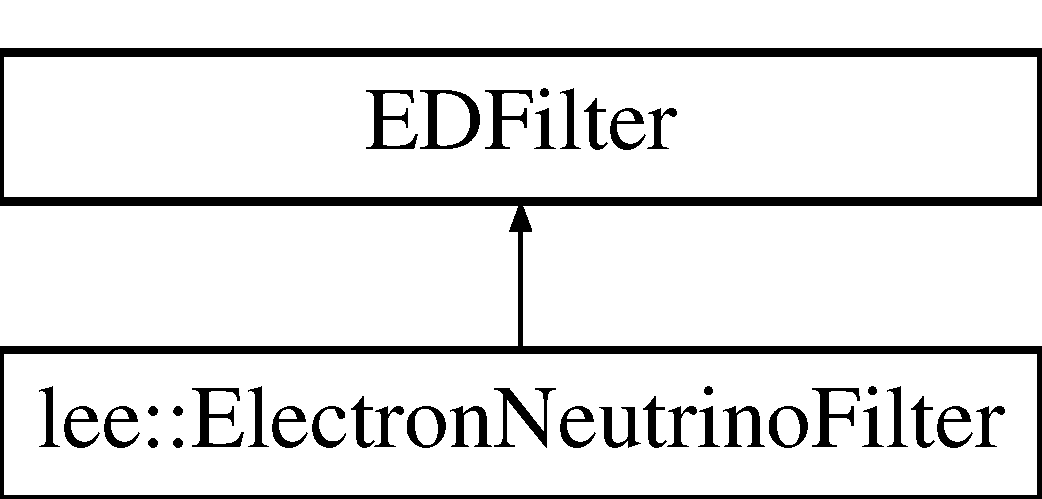
\includegraphics[height=2.000000cm]{classlee_1_1ElectronNeutrinoFilter}
\end{center}
\end{figure}
\subsection*{Public Member Functions}
\begin{DoxyCompactItemize}
\item 
\hypertarget{classlee_1_1ElectronNeutrinoFilter_ad537c8e179a70178666c31f25a1d12d9}{{\bfseries Electron\-Neutrino\-Filter} (fhicl\-::\-Parameter\-Set const \&p)}\label{classlee_1_1ElectronNeutrinoFilter_ad537c8e179a70178666c31f25a1d12d9}

\item 
\hypertarget{classlee_1_1ElectronNeutrinoFilter_a25d84e7ecab146aa6b0e0363b505c961}{{\bfseries Electron\-Neutrino\-Filter} (\hyperlink{classlee_1_1ElectronNeutrinoFilter}{Electron\-Neutrino\-Filter} const \&)=delete}\label{classlee_1_1ElectronNeutrinoFilter_a25d84e7ecab146aa6b0e0363b505c961}

\item 
\hypertarget{classlee_1_1ElectronNeutrinoFilter_a97154ec66a795362acd5f35accf6f7d6}{{\bfseries Electron\-Neutrino\-Filter} (\hyperlink{classlee_1_1ElectronNeutrinoFilter}{Electron\-Neutrino\-Filter} \&\&)=delete}\label{classlee_1_1ElectronNeutrinoFilter_a97154ec66a795362acd5f35accf6f7d6}

\item 
\hypertarget{classlee_1_1ElectronNeutrinoFilter_a3d0689e2f0d746914a8cc9540328df91}{\hyperlink{classlee_1_1ElectronNeutrinoFilter}{Electron\-Neutrino\-Filter} \& {\bfseries operator=} (\hyperlink{classlee_1_1ElectronNeutrinoFilter}{Electron\-Neutrino\-Filter} const \&)=delete}\label{classlee_1_1ElectronNeutrinoFilter_a3d0689e2f0d746914a8cc9540328df91}

\item 
\hypertarget{classlee_1_1ElectronNeutrinoFilter_a14482d0f5624d8671cb0109c3b3f3d5c}{\hyperlink{classlee_1_1ElectronNeutrinoFilter}{Electron\-Neutrino\-Filter} \& {\bfseries operator=} (\hyperlink{classlee_1_1ElectronNeutrinoFilter}{Electron\-Neutrino\-Filter} \&\&)=delete}\label{classlee_1_1ElectronNeutrinoFilter_a14482d0f5624d8671cb0109c3b3f3d5c}

\item 
\hypertarget{classlee_1_1ElectronNeutrinoFilter_a81d6833e781342640df84654c8f7f203}{bool {\bfseries filter} (art\-::\-Event \&e) override}\label{classlee_1_1ElectronNeutrinoFilter_a81d6833e781342640df84654c8f7f203}

\item 
\hypertarget{classlee_1_1ElectronNeutrinoFilter_a891b82ec2e7b2ef034e701cf51a68ac5}{void {\bfseries reconfigure} (fhicl\-::\-Parameter\-Set const \&p) override}\label{classlee_1_1ElectronNeutrinoFilter_a891b82ec2e7b2ef034e701cf51a68ac5}

\item 
\hypertarget{classlee_1_1ElectronNeutrinoFilter_a85815554f7381b9ececc94a83ee86859}{bool {\bfseries end\-Sub\-Run} (art\-::\-Sub\-Run \&sr) override}\label{classlee_1_1ElectronNeutrinoFilter_a85815554f7381b9ececc94a83ee86859}

\end{DoxyCompactItemize}
\subsection*{Private Attributes}
\begin{DoxyCompactItemize}
\item 
\hypertarget{classlee_1_1ElectronNeutrinoFilter_a218cb05b2710a8cfaa9021cc7850bb28}{\hyperlink{classlee_1_1ElectronEventSelectionAlg}{lee\-::\-Electron\-Event\-Selection\-Alg} {\bfseries f\-Electron\-Event\-Selection\-Alg}}\label{classlee_1_1ElectronNeutrinoFilter_a218cb05b2710a8cfaa9021cc7850bb28}

\item 
\hypertarget{classlee_1_1ElectronNeutrinoFilter_ac9531a2782934676b4a5c5562da3139c}{std\-::ofstream {\bfseries \-\_\-run\-\_\-subrun\-\_\-list\-\_\-file}}\label{classlee_1_1ElectronNeutrinoFilter_ac9531a2782934676b4a5c5562da3139c}

\end{DoxyCompactItemize}


The documentation for this class was generated from the following file\-:\begin{DoxyCompactItemize}
\item 
/home/travis/build/soleti/\-Electron\-Neutrino\-Selection/electron\-Neutrino\-Selection/Electron\-Neutrino\-Filter\-\_\-module.\-cc\end{DoxyCompactItemize}

\hypertarget{classEnergyHelper}{\section{Energy\-Helper Class Reference}
\label{classEnergyHelper}\index{Energy\-Helper@{Energy\-Helper}}
}


Helper class with methods accessing calorimetric information (energy and d\-E/dx)  




{\ttfamily \#include $<$Energy\-Helper.\-h$>$}



\subsection{Detailed Description}
Helper class with methods accessing calorimetric information (energy and d\-E/dx) 

\begin{DoxyAuthor}{Author}
Stefano Roberto Soleti \href{mailto:stefano.soleti@physics.ox.ac.uk}{\tt stefano.\-soleti@physics.\-ox.\-ac.\-uk}
\end{DoxyAuthor}
\begin{DoxyDate}{Date}
20/07/2018
\end{DoxyDate}
Contact\-: \href{mailto:stefano.soleti@physics.ox.ac.uk}{\tt stefano.\-soleti@physics.\-ox.\-ac.\-uk}

Created on\-: Fri Jul 20 11\-:20\-:39 2018 

The documentation for this class was generated from the following file\-:\begin{DoxyCompactItemize}
\item 
/home/travis/build/soleti/\-Electron\-Neutrino\-Selection/electron\-Neutrino\-Selection/Energy\-Helper.\-h\end{DoxyCompactItemize}

\hypertarget{classlee_1_1EnergyHelper}{\section{lee\-:\-:Energy\-Helper Class Reference}
\label{classlee_1_1EnergyHelper}\index{lee\-::\-Energy\-Helper@{lee\-::\-Energy\-Helper}}
}
Inheritance diagram for lee\-:\-:Energy\-Helper\-:\begin{figure}[H]
\begin{center}
\leavevmode
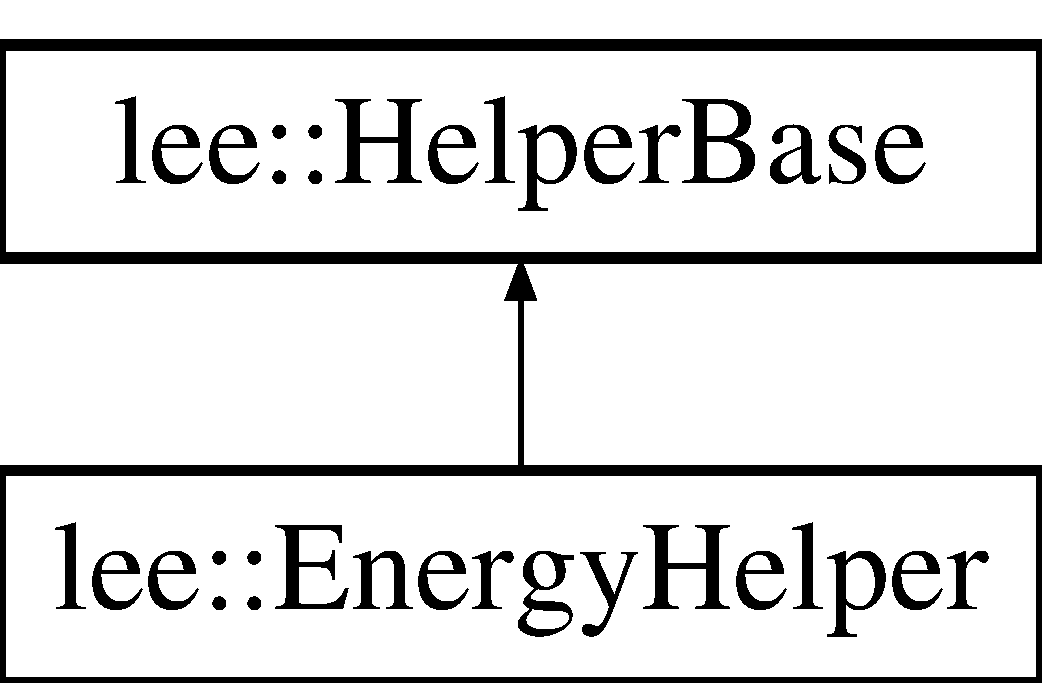
\includegraphics[height=2.000000cm]{classlee_1_1EnergyHelper}
\end{center}
\end{figure}
\subsection*{Public Member Functions}
\begin{DoxyCompactItemize}
\item 
void \hyperlink{group__lee_ga4523185d78d6b7aa94dbf26475750282}{reconfigure} (fhicl\-::\-Parameter\-Set const \&pset)
\begin{DoxyCompactList}\small\item\em Configure all of the parameters of this class. \end{DoxyCompactList}\item 
void \hyperlink{group__lee_ga2da6cbede1c42495e837b3a8b733be48}{d\-Qdx} (const recob\-::\-Shower $\ast$shower\-\_\-obj, std\-::vector$<$ art\-::\-Ptr$<$ recob\-::\-Cluster $>$$>$ $\ast$clusters, art\-::\-Find\-Many\-P$<$ recob\-::\-Hit $>$ $\ast$hits\-\_\-per\-\_\-cluster, std\-::vector$<$ double $>$ \&dqdx, std\-::vector$<$ double $>$ \&dqdx\-\_\-hits, std\-::vector$<$ double $>$ \&pitches, std\-::vector$<$ int $>$ \&dqdx\-\_\-hits\-\_\-in\-\_\-the\-\_\-box)
\begin{DoxyCompactList}\small\item\em Measure the d\-Qdx of a shower. \end{DoxyCompactList}\item 
double \hyperlink{group__lee_ga493326200e39f3aaa22999c55c22b6f5}{P\-I\-D} (const std\-::vector$<$ art\-::\-Ptr$<$ anab\-::\-Particle\-I\-D $>$$>$ $\ast$pids, int track\-I\-D, std\-::string Alg\-Name, anab\-::k\-Variable\-Type Variable\-Type, int pdg\-Code)
\begin{DoxyCompactList}\small\item\em Return the value of a specific Particle\-I\-D algorithm for a single track. \end{DoxyCompactList}\item 
void \hyperlink{group__lee_ga2844c7f27f79fbe5e16d9c674ca4afa1}{d\-Edx\-\_\-from\-\_\-d\-Qdx} (std\-::vector$<$ double $>$ \&dedx, std\-::vector$<$ double $>$ dqdx)
\begin{DoxyCompactList}\small\item\em Convert d\-Q/dx vector into d\-E/dx vector (in Me\-V) \end{DoxyCompactList}\item 
void \hyperlink{group__lee_gac5f41d2b1bee9a0f761179f3059f8a49}{P\-C\-A} (std\-::vector$<$ art\-::\-Ptr$<$ recob\-::\-Cluster $>$$>$ $\ast$clusters, art\-::\-Find\-Many\-P$<$ recob\-::\-Hit $>$ $\ast$hits\-\_\-per\-\_\-cluster, std\-::vector$<$ std\-::vector$<$ double $>$$>$ \&pca\-\_\-planes)
\begin{DoxyCompactList}\small\item\em Principal Component Analysis of reconstructed clusters. \end{DoxyCompactList}\item 
void \hyperlink{group__lee_gaf141846d9be1716bcfcf351633bdf8e7}{get\-\_\-cali} (std\-::vector$<$ art\-::\-Ptr$<$ recob\-::\-Space\-Point $>$$>$ $\ast$spcpnts, art\-::\-Find\-Many\-P$<$ recob\-::\-Hit $>$ $\ast$hits\-\_\-per\-\_\-spcpnts, std\-::vector$<$ double $>$ \&cali\-\_\-corr)
\begin{DoxyCompactList}\small\item\em Calibration value for the energy of a reconstructed object. \end{DoxyCompactList}\item 
void \hyperlink{group__lee_gaabbb21a3db419c9580aec4976c5137a9}{energy\-\_\-from\-\_\-hits} (std\-::vector$<$ art\-::\-Ptr$<$ recob\-::\-Cluster $>$$>$ $\ast$clusters, art\-::\-Find\-Many\-P$<$ recob\-::\-Hit $>$ $\ast$hits\-\_\-per\-\_\-cluster, std\-::vector$<$ int $>$ \&n\-Hits, std\-::vector$<$ double $>$ \&pfenergy)
\begin{DoxyCompactList}\small\item\em Measure calorimetric energy for a reconstructed object. \end{DoxyCompactList}\item 
void \hyperlink{group__lee_ga01205d4a5d2f8d5ad0d4d5462e0b7563}{cluster\-\_\-residuals} (std\-::vector$<$ art\-::\-Ptr$<$ recob\-::\-Cluster $>$$>$ $\ast$clusters, art\-::\-Find\-Many\-P$<$ recob\-::\-Hit $>$ $\ast$hits\-\_\-per\-\_\-cluster, double \&mean\-\_\-v, double \&std\-\_\-v)
\begin{DoxyCompactList}\small\item\em Measure the spatial residuals of the hits in a reconstructed cluster along its direction. \end{DoxyCompactList}\item 
void \hyperlink{group__lee_ga27cd9ba04f447b9922c56bbb320bce08}{track\-\_\-d\-Qdx} (std\-::vector$<$ art\-::\-Ptr$<$ anab\-::\-Calorimetry $>$$>$ $\ast$calos, std\-::vector$<$ double $>$ \&dqdx, std\-::vector$<$ double $>$ \&dedx)
\begin{DoxyCompactList}\small\item\em Measure the d\-Q/dx and d\-E/dx of a track using the anab\-::\-Calorimetry information. \end{DoxyCompactList}\item 
void \hyperlink{group__lee_ga4926738bfba2d91bc187ad8a7db6e997}{d\-Qdx\-\_\-cali} (const recob\-::\-Shower $\ast$shower\-\_\-obj, std\-::vector$<$ double $>$ \&dqdx\-\_\-cali)
\begin{DoxyCompactList}\small\item\em Calibration value for the d\-Q/dx of a reconstructed shower. \end{DoxyCompactList}\end{DoxyCompactItemize}
\subsection*{Private Attributes}
\begin{DoxyCompactItemize}
\item 
\hypertarget{group__lee_gab80c71d066234aa8f0b483c34a068d55}{std\-::vector$<$ double $>$ {\bfseries \-\_\-data\-\_\-gain} = \{236.\-41, 228.\-83, 242.\-72\}}\label{group__lee_gab80c71d066234aa8f0b483c34a068d55}

\item 
\hypertarget{group__lee_ga5c5abe13d6a7820e1658a802790f7e80}{std\-::vector$<$ double $>$ {\bfseries \-\_\-mc\-\_\-gain} = \{193.\-05, 196.\-85, 196.\-85\}}\label{group__lee_ga5c5abe13d6a7820e1658a802790f7e80}

\item 
\hypertarget{group__lee_ga9f16c348e247cda52785e968cfad1b91}{std\-::vector$<$ double $>$ {\bfseries \-\_\-gain}}\label{group__lee_ga9f16c348e247cda52785e968cfad1b91}

\item 
\hypertarget{group__lee_ga4cc0815f3fccf5f704c44fc0a5ed0717}{const \\*
lariov\-::\-T\-P\-C\-Energy\-Calib\-Provider \& {\bfseries \-\_\-energy\-\_\-calib\-\_\-provider} = art\-::\-Service\-Handle$<$lariov\-::\-T\-P\-C\-Energy\-Calib\-Service$>$()-\/$>$Get\-Provider()}\label{group__lee_ga4cc0815f3fccf5f704c44fc0a5ed0717}

\item 
\hypertarget{group__lee_ga5dc96ef9f0d974147c51ca27e46351fa}{const detinfo\-::\-Detector\-Properties $\ast$ {\bfseries \-\_\-detprop} = lar\-::provider\-From$<$detinfo\-::\-Detector\-Properties\-Service$>$()}\label{group__lee_ga5dc96ef9f0d974147c51ca27e46351fa}

\item 
\hypertarget{group__lee_ga5ee65f3a1c672b4f089c05ba6b4ab132}{double {\bfseries \-\_\-drift} = \-\_\-detprop-\/$>$Drift\-Velocity() $\ast$ 1e-\/3}\label{group__lee_ga5ee65f3a1c672b4f089c05ba6b4ab132}

\item 
\hypertarget{group__lee_ga12d5d0f2b40a3971d57e37b1d176e45d}{double {\bfseries \-\_\-from\-\_\-tick\-\_\-to\-\_\-ns} = \-\_\-readout\-\_\-window / \-\_\-detprop-\/$>$Read\-Out\-Window\-Size() $\ast$ 1e6}\label{group__lee_ga12d5d0f2b40a3971d57e37b1d176e45d}

\item 
\hypertarget{group__lee_ga412905c2b45aa8103823f84f7bd7ea2a}{double {\bfseries \-\_\-wire\-\_\-spacing} = 0.\-3}\label{group__lee_ga412905c2b45aa8103823f84f7bd7ea2a}

\item 
\hypertarget{group__lee_gafed9eac818bc9ab7f0c0cd3c808feeea}{double {\bfseries \-\_\-work\-\_\-function} = 23 / 1e6}\label{group__lee_gafed9eac818bc9ab7f0c0cd3c808feeea}

\item 
\hypertarget{group__lee_gad704feff08cf9f09aa46f306e126bbbb}{double {\bfseries \-\_\-readout\-\_\-window}}\label{group__lee_gad704feff08cf9f09aa46f306e126bbbb}

\item 
\hypertarget{group__lee_gafbe2338334b0bb800473d29350d866d1}{double {\bfseries \-\_\-recombination\-\_\-factor}}\label{group__lee_gafbe2338334b0bb800473d29350d866d1}

\item 
\hypertarget{group__lee_gaffce1a06abee9651a41c454aa5f9032f}{double {\bfseries \-\_\-d\-Qdx\-\_\-rectangle\-\_\-length}}\label{group__lee_gaffce1a06abee9651a41c454aa5f9032f}

\item 
\hypertarget{group__lee_ga227149dafb056c355057c753ac768b13}{double {\bfseries \-\_\-d\-Qdx\-\_\-rectangle\-\_\-width}}\label{group__lee_ga227149dafb056c355057c753ac768b13}

\item 
\hypertarget{group__lee_ga613fe58326a28695ad83ddd7bdf8ff57}{\hyperlink{classlee_1_1GeometryHelper}{Geometry\-Helper} {\bfseries geo\-\_\-helper}}\label{group__lee_ga613fe58326a28695ad83ddd7bdf8ff57}

\end{DoxyCompactItemize}


The documentation for this class was generated from the following files\-:\begin{DoxyCompactItemize}
\item 
/home/travis/build/soleti/\-Electron\-Neutrino\-Selection/electron\-Neutrino\-Selection/Energy\-Helper.\-h\item 
/home/travis/build/soleti/\-Electron\-Neutrino\-Selection/electron\-Neutrino\-Selection/Energy\-Helper.\-cxx\end{DoxyCompactItemize}

\hypertarget{classlee_1_1GeometryHelper}{\section{lee\-:\-:Geometry\-Helper Class Reference}
\label{classlee_1_1GeometryHelper}\index{lee\-::\-Geometry\-Helper@{lee\-::\-Geometry\-Helper}}
}
Inheritance diagram for lee\-:\-:Geometry\-Helper\-:\begin{figure}[H]
\begin{center}
\leavevmode
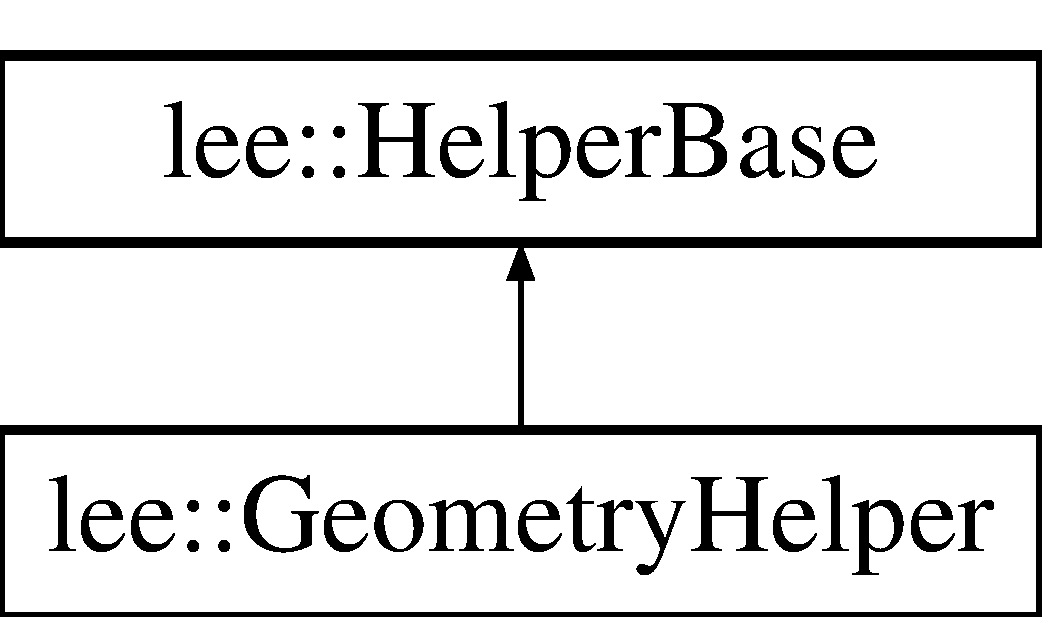
\includegraphics[height=2.000000cm]{classlee_1_1GeometryHelper}
\end{center}
\end{figure}
\subsection*{Public Member Functions}
\begin{DoxyCompactItemize}
\item 
bool \hyperlink{classlee_1_1GeometryHelper_a4d4f0303130ac496452b30f60f43f5f1}{is\-Inside} (std\-::vector$<$ double $>$ P, std\-::vector$<$ std\-::vector$<$ double $>$ $>$ V)
\begin{DoxyCompactList}\small\item\em Determine if a point is within a rectangle (in 2\-D) \end{DoxyCompactList}\item 
bool \hyperlink{classlee_1_1GeometryHelper_a6d02792fc6869b86d850077460536b2a}{is\-Fiducial} (const std\-::vector$<$ double $>$ \&x) const 
\begin{DoxyCompactList}\small\item\em Determine if the specified point is in the fiducial volume. \end{DoxyCompactList}\item 
bool \hyperlink{classlee_1_1GeometryHelper_a5383a8e03c66e9506a75d9afc41f5ff0}{is\-Fiducial} (const T\-Vector3 \&x) const 
\begin{DoxyCompactList}\small\item\em Determine if the specified point is in the fiducial volume. \end{DoxyCompactList}\item 
bool \hyperlink{classlee_1_1GeometryHelper_ae10d0ef387b7573c6cc12565d5bfd0e1}{is\-Fiducial} (const double x\mbox{[}3\mbox{]}) const 
\begin{DoxyCompactList}\small\item\em Determine if the specified point is in the fiducial volume Not recommended, no array size checking is done. \end{DoxyCompactList}\item 
bool \hyperlink{classlee_1_1GeometryHelper_aaa423d79bbb62bdd3337f1d965023baa}{is\-Active} (const std\-::vector$<$ double $>$ \&x) const 
\begin{DoxyCompactList}\small\item\em Determine if the specified point is in the active volume. \end{DoxyCompactList}\item 
bool \hyperlink{classlee_1_1GeometryHelper_ab5c3e840d748f5c5340315b6c096e7c8}{is\-Active} (const double x\mbox{[}3\mbox{]}) const 
\begin{DoxyCompactList}\small\item\em Determine if the specified point is in the active volume Not recommended, no array size checking is done. \end{DoxyCompactList}\item 
double \hyperlink{classlee_1_1GeometryHelper_a15984c2f8c26a4bb9578835bedd19537}{distance} (const std\-::vector$<$ double $>$ \&a, const std\-::vector$<$ double $>$ \&b) const 
\begin{DoxyCompactList}\small\item\em Compute the 3\-D distance between two points. \end{DoxyCompactList}\item 
double \hyperlink{classlee_1_1GeometryHelper_a481ad8eed3b9842a114cce96c73fb02e}{distance} (const T\-Vector3 \&a, const T\-Vector3 \&b) const 
\begin{DoxyCompactList}\small\item\em Compute the 3\-D distance between two points. \end{DoxyCompactList}\item 
double \hyperlink{classlee_1_1GeometryHelper_a02f688ef51442c37a5440d45cfad799f}{get\-Pitch} (const T\-Vector3 \&direction, const int \&pl) const 
\begin{DoxyCompactList}\small\item\em Returns the 3\-D effective pitch give a direction and a plane. \end{DoxyCompactList}\item 
void \hyperlink{classlee_1_1GeometryHelper_a5b67d6d907f9fca0e16ccd9dba85eb54}{set\-Fiducial\-Volume\-Cuts} (float m\-\_\-fidvol\-Xstart, float m\-\_\-fidvol\-Xend, float m\-\_\-fidvol\-Ystart, float m\-\_\-fidvol\-Yend, float m\-\_\-fidvol\-Zstart, float m\-\_\-fidvol\-Zend)
\begin{DoxyCompactList}\small\item\em Sets the fiducial volume cuts. \end{DoxyCompactList}\item 
T\-Vector3 \hyperlink{classlee_1_1GeometryHelper_a1a7546e5a4c1693a9366126ac6c63ba9}{get\-Average\-Position} (std\-::vector$<$ art\-::\-Ptr$<$ recob\-::\-Space\-Point $>$$>$ \&spcpnts)
\begin{DoxyCompactList}\small\item\em Return the average position of a set of space points. \end{DoxyCompactList}\item 
void \hyperlink{classlee_1_1GeometryHelper_a403b726646563c7fa8bce4c316226e15}{build\-Rectangle} (double length, double width, std\-::vector$<$ double $>$ \&start, std\-::vector$<$ double $>$ \&axis, std\-::vector$<$ std\-::vector$<$ double $>$$>$ \&points)
\begin{DoxyCompactList}\small\item\em Builds a rectangle. \end{DoxyCompactList}\end{DoxyCompactItemize}


\subsection{Member Function Documentation}
\hypertarget{classlee_1_1GeometryHelper_a403b726646563c7fa8bce4c316226e15}{\index{lee\-::\-Geometry\-Helper@{lee\-::\-Geometry\-Helper}!build\-Rectangle@{build\-Rectangle}}
\index{build\-Rectangle@{build\-Rectangle}!lee::GeometryHelper@{lee\-::\-Geometry\-Helper}}
\subsubsection[{build\-Rectangle}]{\setlength{\rightskip}{0pt plus 5cm}void Geometry\-Helper\-::build\-Rectangle (
\begin{DoxyParamCaption}
\item[{double}]{length, }
\item[{double}]{width, }
\item[{std\-::vector$<$ double $>$ \&}]{start, }
\item[{std\-::vector$<$ double $>$ \&}]{axis, }
\item[{std\-::vector$<$ std\-::vector$<$ double $>$$>$ \&}]{points}
\end{DoxyParamCaption}
)}}\label{classlee_1_1GeometryHelper_a403b726646563c7fa8bce4c316226e15}


Builds a rectangle. 


\begin{DoxyParams}[1]{Parameters}
\mbox{\tt in}  & {\em length} & The length \\
\hline
\mbox{\tt in}  & {\em width} & The width \\
\hline
 & {\em start} & The start \\
\hline
 & {\em axis} & The axis \\
\hline
 & {\em points} & The points \\
\hline
\end{DoxyParams}
\hypertarget{classlee_1_1GeometryHelper_a15984c2f8c26a4bb9578835bedd19537}{\index{lee\-::\-Geometry\-Helper@{lee\-::\-Geometry\-Helper}!distance@{distance}}
\index{distance@{distance}!lee::GeometryHelper@{lee\-::\-Geometry\-Helper}}
\subsubsection[{distance}]{\setlength{\rightskip}{0pt plus 5cm}double Geometry\-Helper\-::distance (
\begin{DoxyParamCaption}
\item[{const std\-::vector$<$ double $>$ \&}]{a, }
\item[{const std\-::vector$<$ double $>$ \&}]{b}
\end{DoxyParamCaption}
) const}}\label{classlee_1_1GeometryHelper_a15984c2f8c26a4bb9578835bedd19537}


Compute the 3\-D distance between two points. 


\begin{DoxyParams}{Parameters}
{\em a} & First Point \\
\hline
{\em b} & Second Point \\
\hline
\end{DoxyParams}
\begin{DoxyReturn}{Returns}
Returns S\-Q\-R\-T( (a.\-x -\/ b.\-x)$^\wedge$2 + (a.\-y -\/ b.\-y)$^\wedge$2 + (a.\-z -\/ b.\-z)$^\wedge$2 ) 
\end{DoxyReturn}
\hypertarget{classlee_1_1GeometryHelper_a481ad8eed3b9842a114cce96c73fb02e}{\index{lee\-::\-Geometry\-Helper@{lee\-::\-Geometry\-Helper}!distance@{distance}}
\index{distance@{distance}!lee::GeometryHelper@{lee\-::\-Geometry\-Helper}}
\subsubsection[{distance}]{\setlength{\rightskip}{0pt plus 5cm}double Geometry\-Helper\-::distance (
\begin{DoxyParamCaption}
\item[{const T\-Vector3 \&}]{a, }
\item[{const T\-Vector3 \&}]{b}
\end{DoxyParamCaption}
) const}}\label{classlee_1_1GeometryHelper_a481ad8eed3b9842a114cce96c73fb02e}


Compute the 3\-D distance between two points. 


\begin{DoxyParams}{Parameters}
{\em a} & First Point \\
\hline
{\em b} & Second Point \\
\hline
\end{DoxyParams}
\begin{DoxyReturn}{Returns}
Returns S\-Q\-R\-T( (a.\-x -\/ b.\-x)$^\wedge$2 + (a.\-y -\/ b.\-y)$^\wedge$2 + (a.\-z -\/ b.\-z)$^\wedge$2 ) 
\end{DoxyReturn}
\hypertarget{classlee_1_1GeometryHelper_a1a7546e5a4c1693a9366126ac6c63ba9}{\index{lee\-::\-Geometry\-Helper@{lee\-::\-Geometry\-Helper}!get\-Average\-Position@{get\-Average\-Position}}
\index{get\-Average\-Position@{get\-Average\-Position}!lee::GeometryHelper@{lee\-::\-Geometry\-Helper}}
\subsubsection[{get\-Average\-Position}]{\setlength{\rightskip}{0pt plus 5cm}T\-Vector3 Geometry\-Helper\-::get\-Average\-Position (
\begin{DoxyParamCaption}
\item[{std\-::vector$<$ art\-::\-Ptr$<$ recob\-::\-Space\-Point $>$$>$ \&}]{spcpnts}
\end{DoxyParamCaption}
)}}\label{classlee_1_1GeometryHelper_a1a7546e5a4c1693a9366126ac6c63ba9}


Return the average position of a set of space points. 


\begin{DoxyParams}{Parameters}
{\em spcpnts} & The spcpnts\\
\hline
\end{DoxyParams}
\begin{DoxyReturn}{Returns}
3\-D Vector 
\end{DoxyReturn}
\hypertarget{classlee_1_1GeometryHelper_a02f688ef51442c37a5440d45cfad799f}{\index{lee\-::\-Geometry\-Helper@{lee\-::\-Geometry\-Helper}!get\-Pitch@{get\-Pitch}}
\index{get\-Pitch@{get\-Pitch}!lee::GeometryHelper@{lee\-::\-Geometry\-Helper}}
\subsubsection[{get\-Pitch}]{\setlength{\rightskip}{0pt plus 5cm}double Geometry\-Helper\-::get\-Pitch (
\begin{DoxyParamCaption}
\item[{const T\-Vector3 \&}]{direction, }
\item[{const int \&}]{pl}
\end{DoxyParamCaption}
) const}}\label{classlee_1_1GeometryHelper_a02f688ef51442c37a5440d45cfad799f}


Returns the 3\-D effective pitch give a direction and a plane. 


\begin{DoxyParams}[1]{Parameters}
\mbox{\tt in}  & {\em direction} & The direction \\
\hline
\mbox{\tt in}  & {\em pl} & Plane of interest (0, 1, 2)\\
\hline
\end{DoxyParams}
\begin{DoxyReturn}{Returns}
The pitch. 
\end{DoxyReturn}
\hypertarget{classlee_1_1GeometryHelper_aaa423d79bbb62bdd3337f1d965023baa}{\index{lee\-::\-Geometry\-Helper@{lee\-::\-Geometry\-Helper}!is\-Active@{is\-Active}}
\index{is\-Active@{is\-Active}!lee::GeometryHelper@{lee\-::\-Geometry\-Helper}}
\subsubsection[{is\-Active}]{\setlength{\rightskip}{0pt plus 5cm}bool Geometry\-Helper\-::is\-Active (
\begin{DoxyParamCaption}
\item[{const std\-::vector$<$ double $>$ \&}]{x}
\end{DoxyParamCaption}
) const}}\label{classlee_1_1GeometryHelper_aaa423d79bbb62bdd3337f1d965023baa}


Determine if the specified point is in the active volume. 


\begin{DoxyParams}{Parameters}
{\em x} & array of 3\-D location \\
\hline
\end{DoxyParams}
\begin{DoxyReturn}{Returns}
True or false 
\end{DoxyReturn}
\hypertarget{classlee_1_1GeometryHelper_ab5c3e840d748f5c5340315b6c096e7c8}{\index{lee\-::\-Geometry\-Helper@{lee\-::\-Geometry\-Helper}!is\-Active@{is\-Active}}
\index{is\-Active@{is\-Active}!lee::GeometryHelper@{lee\-::\-Geometry\-Helper}}
\subsubsection[{is\-Active}]{\setlength{\rightskip}{0pt plus 5cm}bool Geometry\-Helper\-::is\-Active (
\begin{DoxyParamCaption}
\item[{const double}]{x\mbox{[}3\mbox{]}}
\end{DoxyParamCaption}
) const}}\label{classlee_1_1GeometryHelper_ab5c3e840d748f5c5340315b6c096e7c8}


Determine if the specified point is in the active volume Not recommended, no array size checking is done. 


\begin{DoxyParams}{Parameters}
{\em x} & array of 3\-D location \\
\hline
\end{DoxyParams}
\begin{DoxyReturn}{Returns}
True or false 
\end{DoxyReturn}
\hypertarget{classlee_1_1GeometryHelper_a6d02792fc6869b86d850077460536b2a}{\index{lee\-::\-Geometry\-Helper@{lee\-::\-Geometry\-Helper}!is\-Fiducial@{is\-Fiducial}}
\index{is\-Fiducial@{is\-Fiducial}!lee::GeometryHelper@{lee\-::\-Geometry\-Helper}}
\subsubsection[{is\-Fiducial}]{\setlength{\rightskip}{0pt plus 5cm}bool Geometry\-Helper\-::is\-Fiducial (
\begin{DoxyParamCaption}
\item[{const std\-::vector$<$ double $>$ \&}]{x}
\end{DoxyParamCaption}
) const}}\label{classlee_1_1GeometryHelper_a6d02792fc6869b86d850077460536b2a}


Determine if the specified point is in the fiducial volume. 


\begin{DoxyParams}{Parameters}
{\em x} & vector of length 3 \\
\hline
\end{DoxyParams}
\begin{DoxyReturn}{Returns}
True or false 
\end{DoxyReturn}
\hypertarget{classlee_1_1GeometryHelper_a5383a8e03c66e9506a75d9afc41f5ff0}{\index{lee\-::\-Geometry\-Helper@{lee\-::\-Geometry\-Helper}!is\-Fiducial@{is\-Fiducial}}
\index{is\-Fiducial@{is\-Fiducial}!lee::GeometryHelper@{lee\-::\-Geometry\-Helper}}
\subsubsection[{is\-Fiducial}]{\setlength{\rightskip}{0pt plus 5cm}bool Geometry\-Helper\-::is\-Fiducial (
\begin{DoxyParamCaption}
\item[{const T\-Vector3 \&}]{x}
\end{DoxyParamCaption}
) const}}\label{classlee_1_1GeometryHelper_a5383a8e03c66e9506a75d9afc41f5ff0}


Determine if the specified point is in the fiducial volume. 


\begin{DoxyParams}{Parameters}
{\em x} & T\-Vector3 of 3\-D location \\
\hline
\end{DoxyParams}
\begin{DoxyReturn}{Returns}
True or false 
\end{DoxyReturn}
\hypertarget{classlee_1_1GeometryHelper_ae10d0ef387b7573c6cc12565d5bfd0e1}{\index{lee\-::\-Geometry\-Helper@{lee\-::\-Geometry\-Helper}!is\-Fiducial@{is\-Fiducial}}
\index{is\-Fiducial@{is\-Fiducial}!lee::GeometryHelper@{lee\-::\-Geometry\-Helper}}
\subsubsection[{is\-Fiducial}]{\setlength{\rightskip}{0pt plus 5cm}bool Geometry\-Helper\-::is\-Fiducial (
\begin{DoxyParamCaption}
\item[{const double}]{x\mbox{[}3\mbox{]}}
\end{DoxyParamCaption}
) const}}\label{classlee_1_1GeometryHelper_ae10d0ef387b7573c6cc12565d5bfd0e1}


Determine if the specified point is in the fiducial volume Not recommended, no array size checking is done. 


\begin{DoxyParams}{Parameters}
{\em x} & array of 3\-D location \\
\hline
\end{DoxyParams}
\begin{DoxyReturn}{Returns}
True or false 
\end{DoxyReturn}
\hypertarget{classlee_1_1GeometryHelper_a4d4f0303130ac496452b30f60f43f5f1}{\index{lee\-::\-Geometry\-Helper@{lee\-::\-Geometry\-Helper}!is\-Inside@{is\-Inside}}
\index{is\-Inside@{is\-Inside}!lee::GeometryHelper@{lee\-::\-Geometry\-Helper}}
\subsubsection[{is\-Inside}]{\setlength{\rightskip}{0pt plus 5cm}bool Geometry\-Helper\-::is\-Inside (
\begin{DoxyParamCaption}
\item[{std\-::vector$<$ double $>$}]{P, }
\item[{std\-::vector$<$ std\-::vector$<$ double $>$ $>$}]{V}
\end{DoxyParamCaption}
)}}\label{classlee_1_1GeometryHelper_a4d4f0303130ac496452b30f60f43f5f1}


Determine if a point is within a rectangle (in 2\-D) 


\begin{DoxyParams}{Parameters}
{\em P} & vector containing the point's coordinates \\
\hline
{\em V} & vector of vectors containing rectangle's vertices\\
\hline
\end{DoxyParams}
\begin{DoxyReturn}{Returns}
True if the points is inside, False otherwise 
\end{DoxyReturn}
\hypertarget{classlee_1_1GeometryHelper_a5b67d6d907f9fca0e16ccd9dba85eb54}{\index{lee\-::\-Geometry\-Helper@{lee\-::\-Geometry\-Helper}!set\-Fiducial\-Volume\-Cuts@{set\-Fiducial\-Volume\-Cuts}}
\index{set\-Fiducial\-Volume\-Cuts@{set\-Fiducial\-Volume\-Cuts}!lee::GeometryHelper@{lee\-::\-Geometry\-Helper}}
\subsubsection[{set\-Fiducial\-Volume\-Cuts}]{\setlength{\rightskip}{0pt plus 5cm}void Geometry\-Helper\-::set\-Fiducial\-Volume\-Cuts (
\begin{DoxyParamCaption}
\item[{float}]{m\-\_\-fidvol\-Xstart, }
\item[{float}]{m\-\_\-fidvol\-Xend, }
\item[{float}]{m\-\_\-fidvol\-Ystart, }
\item[{float}]{m\-\_\-fidvol\-Yend, }
\item[{float}]{m\-\_\-fidvol\-Zstart, }
\item[{float}]{m\-\_\-fidvol\-Zend}
\end{DoxyParamCaption}
)}}\label{classlee_1_1GeometryHelper_a5b67d6d907f9fca0e16ccd9dba85eb54}


Sets the fiducial volume cuts. 


\begin{DoxyParams}[1]{Parameters}
\mbox{\tt in}  & {\em m\-\_\-fidvol\-Xstart} & The x start \\
\hline
\mbox{\tt in}  & {\em m\-\_\-fidvol\-Xend} & The x end \\
\hline
\mbox{\tt in}  & {\em m\-\_\-fidvol\-Ystart} & The y start \\
\hline
\mbox{\tt in}  & {\em m\-\_\-fidvol\-Yend} & The y end \\
\hline
\mbox{\tt in}  & {\em m\-\_\-fidvol\-Zstart} & The z start \\
\hline
\mbox{\tt in}  & {\em m\-\_\-fidvol\-Zend} & The z end \\
\hline
\end{DoxyParams}


The documentation for this class was generated from the following files\-:\begin{DoxyCompactItemize}
\item 
/home/travis/build/soleti/\-Electron\-Neutrino\-Selection/electron\-Neutrino\-Selection/Geometry\-Helper.\-h\item 
/home/travis/build/soleti/\-Electron\-Neutrino\-Selection/electron\-Neutrino\-Selection/Geometry\-Helper.\-cxx\end{DoxyCompactItemize}

\hypertarget{classGeometryHelper}{\section{Geometry\-Helper Class Reference}
\label{classGeometryHelper}\index{Geometry\-Helper@{Geometry\-Helper}}
}


Helper class with geometric methods (distance, point in a plane, etc. )  




{\ttfamily \#include $<$Geometry\-Helper.\-h$>$}



\subsection{Detailed Description}
Helper class with geometric methods (distance, point in a plane, etc. ) 

\begin{DoxyAuthor}{Author}
Stefano Roberto Soleti \href{mailto:stefano.soleti@physics.ox.ac.uk}{\tt stefano.\-soleti@physics.\-ox.\-ac.\-uk}
\end{DoxyAuthor}
\begin{DoxyDate}{Date}
20/07/2018
\end{DoxyDate}
Contact\-: \href{mailto:stefano.soleti@physics.ox.ac.uk}{\tt stefano.\-soleti@physics.\-ox.\-ac.\-uk}

Created on\-: Fri Jul 20 11\-:20\-:39 2018 

The documentation for this class was generated from the following file\-:\begin{DoxyCompactItemize}
\item 
/home/travis/build/soleti/\-Electron\-Neutrino\-Selection/electron\-Neutrino\-Selection/Geometry\-Helper.\-h\end{DoxyCompactItemize}

\hypertarget{classlee_1_1HelperBase}{\section{lee\-:\-:Helper\-Base Class Reference}
\label{classlee_1_1HelperBase}\index{lee\-::\-Helper\-Base@{lee\-::\-Helper\-Base}}
}
Inheritance diagram for lee\-:\-:Helper\-Base\-:\begin{figure}[H]
\begin{center}
\leavevmode
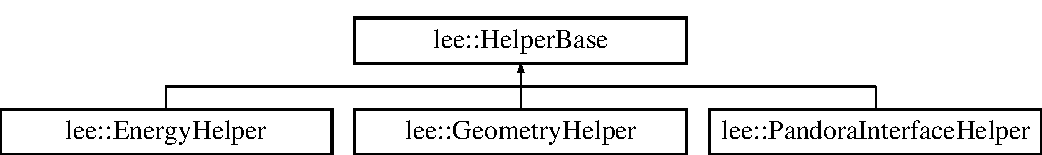
\includegraphics[height=2.000000cm]{classlee_1_1HelperBase}
\end{center}
\end{figure}
\subsection*{Public Member Functions}
\begin{DoxyCompactItemize}
\item 
void \hyperlink{classlee_1_1HelperBase_ad80955b099f76d5e298e6f5e37cd17aa}{set\-Debug} (bool b)
\begin{DoxyCompactList}\small\item\em Sets the debug parameter. \end{DoxyCompactList}\end{DoxyCompactItemize}


\subsection{Member Function Documentation}
\hypertarget{classlee_1_1HelperBase_ad80955b099f76d5e298e6f5e37cd17aa}{\index{lee\-::\-Helper\-Base@{lee\-::\-Helper\-Base}!set\-Debug@{set\-Debug}}
\index{set\-Debug@{set\-Debug}!lee::HelperBase@{lee\-::\-Helper\-Base}}
\subsubsection[{set\-Debug}]{\setlength{\rightskip}{0pt plus 5cm}void lee\-::\-Helper\-Base\-::set\-Debug (
\begin{DoxyParamCaption}
\item[{bool}]{b}
\end{DoxyParamCaption}
)\hspace{0.3cm}{\ttfamily [inline]}}}\label{classlee_1_1HelperBase_ad80955b099f76d5e298e6f5e37cd17aa}


Sets the debug parameter. 


\begin{DoxyParams}[1]{Parameters}
\mbox{\tt in}  & {\em b} & Boolean, debug parameter O\-N (true) or O\-F\-F (false) \\
\hline
\end{DoxyParams}


The documentation for this class was generated from the following file\-:\begin{DoxyCompactItemize}
\item 
/home/travis/build/soleti/\-Electron\-Neutrino\-Selection/electron\-Neutrino\-Selection/Helper\-Base.\-h\end{DoxyCompactItemize}

\hypertarget{classPandoraInterfaceHelper}{\section{Pandora\-Interface\-Helper Class Reference}
\label{classPandoraInterfaceHelper}\index{Pandora\-Interface\-Helper@{Pandora\-Interface\-Helper}}
}


Helper class with methods useful to interface with Pandora information. It contains the methods use to perform reco/true matching.  




{\ttfamily \#include $<$Pandora\-Interface\-Helper.\-h$>$}



\subsection{Detailed Description}
Helper class with methods useful to interface with Pandora information. It contains the methods use to perform reco/true matching. 

\begin{DoxyAuthor}{Author}
Stefano Roberto Soleti \href{mailto:stefano.soleti@physics.ox.ac.uk}{\tt stefano.\-soleti@physics.\-ox.\-ac.\-uk}
\end{DoxyAuthor}
\begin{DoxyDate}{Date}
20/07/2018
\end{DoxyDate}
Contact\-: \href{mailto:stefano.soleti@physics.ox.ac.uk}{\tt stefano.\-soleti@physics.\-ox.\-ac.\-uk}

Created on\-: Fri Jul 20 11\-:20\-:39 2018 

The documentation for this class was generated from the following file\-:\begin{DoxyCompactItemize}
\item 
/home/travis/build/soleti/\-Electron\-Neutrino\-Selection/electron\-Neutrino\-Selection/Pandora\-Interface\-Helper.\-h\end{DoxyCompactItemize}

\hypertarget{classlee_1_1PandoraInterfaceHelper}{\section{lee\-:\-:Pandora\-Interface\-Helper Class Reference}
\label{classlee_1_1PandoraInterfaceHelper}\index{lee\-::\-Pandora\-Interface\-Helper@{lee\-::\-Pandora\-Interface\-Helper}}
}
Inheritance diagram for lee\-:\-:Pandora\-Interface\-Helper\-:\begin{figure}[H]
\begin{center}
\leavevmode
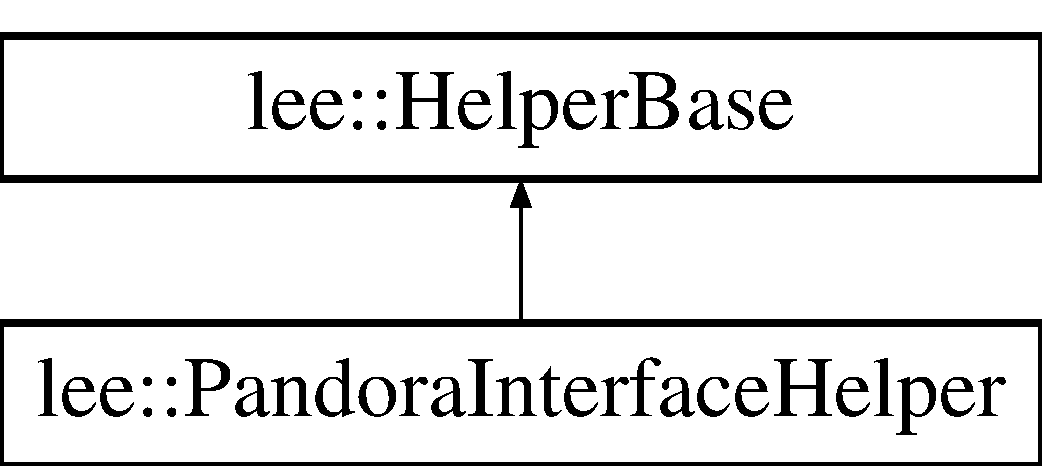
\includegraphics[height=2.000000cm]{classlee_1_1PandoraInterfaceHelper}
\end{center}
\end{figure}
\subsection*{Public Member Functions}
\begin{DoxyCompactItemize}
\item 
void \hyperlink{classlee_1_1PandoraInterfaceHelper_a43b81ca3b961e30d191ebc53f987cf2a}{traverse\-P\-F\-Particle\-Tree} (const art\-::\-Valid\-Handle$<$ std\-::vector$<$ recob\-::\-P\-F\-Particle $>$$>$ pfparticles, size\-\_\-t top\-\_\-index, std\-::vector$<$ size\-\_\-t $>$ \&unordered\-\_\-daugthers, std\-::string \-\_\-pfp\-\_\-producer)
\begin{DoxyCompactList}\small\item\em Travers the tree of the daughters of a P\-F\-Particle. \end{DoxyCompactList}\item 
std\-::vector$<$ double $>$ \hyperlink{classlee_1_1PandoraInterfaceHelper_a5434c10225e008643b7b9a48fd2e9bea}{calculate\-Charge\-Center} (size\-\_\-t ipf, const art\-::\-Valid\-Handle$<$ std\-::vector$<$ recob\-::\-P\-F\-Particle $>$$>$ pfparticles, const art\-::\-Event \&evt, std\-::string \-\_\-pfp\-\_\-producer)
\begin{DoxyCompactList}\small\item\em Measures the three-\/dimensional center of the deposited charge for a P\-F\-Particle. \end{DoxyCompactList}\item 
\hypertarget{classlee_1_1PandoraInterfaceHelper_ab0c4a8fd1bac60bb44cd26e0541feffa}{void {\bfseries get\-\_\-daughter\-\_\-tracks} (std\-::vector$<$ size\-\_\-t $>$ pf\-\_\-ids, const art\-::\-Event \&evt, std\-::vector$<$ art\-::\-Ptr$<$ recob\-::\-Track $>$$>$ \&tracks, std\-::string \-\_\-pfp\-\_\-producer)}\label{classlee_1_1PandoraInterfaceHelper_ab0c4a8fd1bac60bb44cd26e0541feffa}

\item 
\hypertarget{classlee_1_1PandoraInterfaceHelper_a89f77d090524bc3060a40330635527d5}{void {\bfseries get\-\_\-daughter\-\_\-showers} (std\-::vector$<$ size\-\_\-t $>$ pf\-\_\-ids, const art\-::\-Event \&evt, std\-::vector$<$ art\-::\-Ptr$<$ recob\-::\-Shower $>$$>$ \&showers, std\-::string \-\_\-pfp\-\_\-producer)}\label{classlee_1_1PandoraInterfaceHelper_a89f77d090524bc3060a40330635527d5}

\item 
void \hyperlink{classlee_1_1PandoraInterfaceHelper_a7c248af2e489ded3723275cd0a13a6ff}{Get\-Reco\-To\-True\-Matches} (lar\-\_\-pandora\-::\-P\-F\-Particles\-To\-M\-C\-Particles \&matched\-Particles)
\begin{DoxyCompactList}\small\item\em Configure function parameters. \end{DoxyCompactList}\item 
\hypertarget{classlee_1_1PandoraInterfaceHelper_a183d7e49018d16cb37d7fc299ad7ede1}{void {\bfseries Configure} (art\-::\-Event const \&e, std\-::string \-\_\-pfp\-\_\-producer, std\-::string \-\_\-spacepoint\-\_\-producer, std\-::string \-\_\-hitfinder\-\_\-producer, std\-::string \-\_\-geant\-\_\-producer, std\-::string \-\_\-hit\-\_\-mcp\-\_\-producer)}\label{classlee_1_1PandoraInterfaceHelper_a183d7e49018d16cb37d7fc299ad7ede1}

\item 
\hypertarget{classlee_1_1PandoraInterfaceHelper_a47c1f51234888908d4027cdc8e89972c}{art\-::\-Ptr$<$ simb\-::\-M\-C\-Truth $>$ {\bfseries Track\-I\-D\-To\-M\-C\-Truth} (art\-::\-Event const \&e, std\-::string \-\_\-geant\-\_\-producer, int geant\-\_\-track\-\_\-id)}\label{classlee_1_1PandoraInterfaceHelper_a47c1f51234888908d4027cdc8e89972c}

\end{DoxyCompactItemize}
\subsection*{Protected Attributes}
\begin{DoxyCompactItemize}
\item 
\hypertarget{classlee_1_1PandoraInterfaceHelper_add430a976fa40632e14eb1688cdd785b}{lar\-\_\-pandora\-::\-Hits\-To\-M\-C\-Particles \hyperlink{classlee_1_1PandoraInterfaceHelper_add430a976fa40632e14eb1688cdd785b}{\-\_\-hit\-\_\-to\-\_\-mcps\-\_\-map}}\label{classlee_1_1PandoraInterfaceHelper_add430a976fa40632e14eb1688cdd785b}

\begin{DoxyCompactList}\small\item\em A map from recon hits to M\-C\-Particles. \end{DoxyCompactList}\item 
\hypertarget{classlee_1_1PandoraInterfaceHelper_ae19df94cb2c29dc2735bf7436c5ccf63}{lar\-\_\-pandora\-::\-P\-F\-Particles\-To\-Hits \hyperlink{classlee_1_1PandoraInterfaceHelper_ae19df94cb2c29dc2735bf7436c5ccf63}{\-\_\-pfp\-\_\-to\-\_\-hits\-\_\-map}}\label{classlee_1_1PandoraInterfaceHelper_ae19df94cb2c29dc2735bf7436c5ccf63}

\begin{DoxyCompactList}\small\item\em A map from P\-F\-Particles to recon hits. \end{DoxyCompactList}\end{DoxyCompactItemize}


\subsection{Member Function Documentation}
\hypertarget{classlee_1_1PandoraInterfaceHelper_a5434c10225e008643b7b9a48fd2e9bea}{\index{lee\-::\-Pandora\-Interface\-Helper@{lee\-::\-Pandora\-Interface\-Helper}!calculate\-Charge\-Center@{calculate\-Charge\-Center}}
\index{calculate\-Charge\-Center@{calculate\-Charge\-Center}!lee::PandoraInterfaceHelper@{lee\-::\-Pandora\-Interface\-Helper}}
\subsubsection[{calculate\-Charge\-Center}]{\setlength{\rightskip}{0pt plus 5cm}std\-::vector$<$ double $>$ lee\-::\-Pandora\-Interface\-Helper\-::calculate\-Charge\-Center (
\begin{DoxyParamCaption}
\item[{size\-\_\-t}]{ipf, }
\item[{const art\-::\-Valid\-Handle$<$ std\-::vector$<$ recob\-::\-P\-F\-Particle $>$$>$}]{pfparticles, }
\item[{const art\-::\-Event \&}]{evt, }
\item[{std\-::string}]{\-\_\-pfp\-\_\-producer}
\end{DoxyParamCaption}
)}}\label{classlee_1_1PandoraInterfaceHelper_a5434c10225e008643b7b9a48fd2e9bea}


Measures the three-\/dimensional center of the deposited charge for a P\-F\-Particle. 


\begin{DoxyParams}{Parameters}
{\em ipf} & Index of the P\-F\-Particle \\
\hline
{\em pfparticles} & P\-F\-Particles handle \\
\hline
{\em evt} & art Event \\
\hline
\end{DoxyParams}
\begin{DoxyReturn}{Returns}
vector with\-: lowest x\-\_\-sps, center in y, z, and total deposited charge on the collection plane. 
\end{DoxyReturn}
\hypertarget{classlee_1_1PandoraInterfaceHelper_a7c248af2e489ded3723275cd0a13a6ff}{\index{lee\-::\-Pandora\-Interface\-Helper@{lee\-::\-Pandora\-Interface\-Helper}!Get\-Reco\-To\-True\-Matches@{Get\-Reco\-To\-True\-Matches}}
\index{Get\-Reco\-To\-True\-Matches@{Get\-Reco\-To\-True\-Matches}!lee::PandoraInterfaceHelper@{lee\-::\-Pandora\-Interface\-Helper}}
\subsubsection[{Get\-Reco\-To\-True\-Matches}]{\setlength{\rightskip}{0pt plus 5cm}void lee\-::\-Pandora\-Interface\-Helper\-::\-Get\-Reco\-To\-True\-Matches (
\begin{DoxyParamCaption}
\item[{lar\-\_\-pandora\-::\-P\-F\-Particles\-To\-M\-C\-Particles \&}]{matched\-Particles}
\end{DoxyParamCaption}
)}}\label{classlee_1_1PandoraInterfaceHelper_a7c248af2e489ded3723275cd0a13a6ff}


Configure function parameters. 

Configure function parameters (call this function first)


\begin{DoxyParams}{Parameters}
{\em e} & the art\-::\-Event \\
\hline
{\em \-\_\-pfp\-\_\-producer} & the P\-F\-Particle producer label \\
\hline
{\em \-\_\-spacepoint\-\_\-producer} & the Space\-Point producer label \\
\hline
{\em \-\_\-hitfinder\-\_\-producer} & the Hit producer label \\
\hline
{\em \-\_\-geant\-\_\-producer} & The Geant4 producer label Returns matching between true and reconstructed particles\\
\hline
{\em matched\-Particles} & the output matches between reconstructed and true particles \\
\hline
\end{DoxyParams}
\hypertarget{classlee_1_1PandoraInterfaceHelper_a43b81ca3b961e30d191ebc53f987cf2a}{\index{lee\-::\-Pandora\-Interface\-Helper@{lee\-::\-Pandora\-Interface\-Helper}!traverse\-P\-F\-Particle\-Tree@{traverse\-P\-F\-Particle\-Tree}}
\index{traverse\-P\-F\-Particle\-Tree@{traverse\-P\-F\-Particle\-Tree}!lee::PandoraInterfaceHelper@{lee\-::\-Pandora\-Interface\-Helper}}
\subsubsection[{traverse\-P\-F\-Particle\-Tree}]{\setlength{\rightskip}{0pt plus 5cm}void lee\-::\-Pandora\-Interface\-Helper\-::traverse\-P\-F\-Particle\-Tree (
\begin{DoxyParamCaption}
\item[{const art\-::\-Valid\-Handle$<$ std\-::vector$<$ recob\-::\-P\-F\-Particle $>$$>$}]{pfparticles, }
\item[{size\-\_\-t}]{top\-\_\-index, }
\item[{std\-::vector$<$ size\-\_\-t $>$ \&}]{unordered\-\_\-daugthers, }
\item[{std\-::string}]{\-\_\-pfp\-\_\-producer}
\end{DoxyParamCaption}
)}}\label{classlee_1_1PandoraInterfaceHelper_a43b81ca3b961e30d191ebc53f987cf2a}


Travers the tree of the daughters of a P\-F\-Particle. 


\begin{DoxyParams}{Parameters}
{\em pfparticles} & P\-F\-Particles handle \\
\hline
{\em top\-\_\-index} & Index of the parent \\
\hline
{\em unordered\-\_\-daugthers} & Vector of P\-F\-Particles daughters \\
\hline
\end{DoxyParams}


The documentation for this class was generated from the following files\-:\begin{DoxyCompactItemize}
\item 
/home/travis/build/soleti/\-Electron\-Neutrino\-Selection/electron\-Neutrino\-Selection/Pandora\-Interface\-Helper.\-h\item 
/home/travis/build/soleti/\-Electron\-Neutrino\-Selection/electron\-Neutrino\-Selection/Pandora\-Interface\-Helper.\-cxx\end{DoxyCompactItemize}

\hypertarget{classlee_1_1PandoraLEEAnalyzer}{\section{lee\-:\-:Pandora\-L\-E\-E\-Analyzer Class Reference}
\label{classlee_1_1PandoraLEEAnalyzer}\index{lee\-::\-Pandora\-L\-E\-E\-Analyzer@{lee\-::\-Pandora\-L\-E\-E\-Analyzer}}
}
Inheritance diagram for lee\-:\-:Pandora\-L\-E\-E\-Analyzer\-:\begin{figure}[H]
\begin{center}
\leavevmode
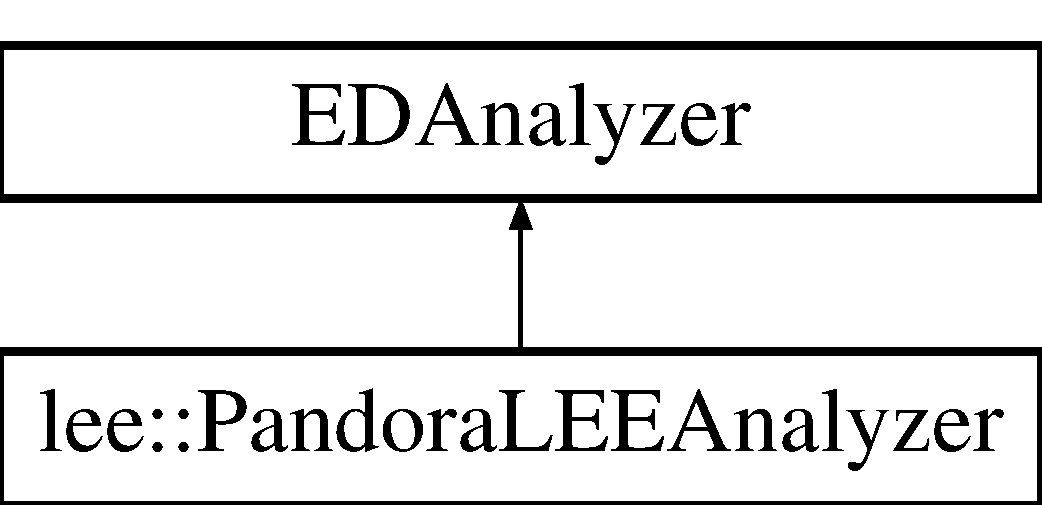
\includegraphics[height=2.000000cm]{classlee_1_1PandoraLEEAnalyzer}
\end{center}
\end{figure}
\subsection*{Public Member Functions}
\begin{DoxyCompactItemize}
\item 
\hypertarget{group__lee_ga3783391baff0585de9261a559a8d28ef}{{\bfseries Pandora\-L\-E\-E\-Analyzer} (fhicl\-::\-Parameter\-Set const \&pset)}\label{group__lee_ga3783391baff0585de9261a559a8d28ef}

\item 
\hypertarget{group__lee_ga50f8e3ecdc7892d554c68080645af88c}{{\bfseries Pandora\-L\-E\-E\-Analyzer} (\hyperlink{classlee_1_1PandoraLEEAnalyzer}{Pandora\-L\-E\-E\-Analyzer} const \&)=delete}\label{group__lee_ga50f8e3ecdc7892d554c68080645af88c}

\item 
\hypertarget{group__lee_ga8e9dc3f96fcb2881bee2bfb46dcedaaf}{{\bfseries Pandora\-L\-E\-E\-Analyzer} (\hyperlink{classlee_1_1PandoraLEEAnalyzer}{Pandora\-L\-E\-E\-Analyzer} \&\&)=delete}\label{group__lee_ga8e9dc3f96fcb2881bee2bfb46dcedaaf}

\item 
\hypertarget{group__lee_gae71d8ba45ecaaa09a587ecf3cd693675}{\hyperlink{classlee_1_1PandoraLEEAnalyzer}{Pandora\-L\-E\-E\-Analyzer} \& {\bfseries operator=} (\hyperlink{classlee_1_1PandoraLEEAnalyzer}{Pandora\-L\-E\-E\-Analyzer} const \&)=delete}\label{group__lee_gae71d8ba45ecaaa09a587ecf3cd693675}

\item 
\hypertarget{group__lee_ga79984f454c76dbb927254731d85e40c4}{\hyperlink{classlee_1_1PandoraLEEAnalyzer}{Pandora\-L\-E\-E\-Analyzer} \& {\bfseries operator=} (\hyperlink{classlee_1_1PandoraLEEAnalyzer}{Pandora\-L\-E\-E\-Analyzer} \&\&)=delete}\label{group__lee_ga79984f454c76dbb927254731d85e40c4}

\item 
void \hyperlink{group__lee_gab6142fdaa2037d01df2304cbb17d59b0}{analyze} (art\-::\-Event const \&e) override
\begin{DoxyCompactList}\small\item\em Main analyzer method, runs for every event in the file. \end{DoxyCompactList}\item 
void \hyperlink{group__lee_gaede981b7ff7b78309f2457c40581ba71}{end\-Sub\-Run} (const art\-::\-Sub\-Run \&sr)
\begin{DoxyCompactList}\small\item\em Method called at the end of each subrun, it stores the number of P\-O\-T. \end{DoxyCompactList}\item 
void \hyperlink{group__lee_ga4696139a07194b86735e93fe0d9df45e}{reconfigure} (fhicl\-::\-Parameter\-Set const \&pset) override
\begin{DoxyCompactList}\small\item\em Assigns the values of the F\-H\-I\-C\-L file. \end{DoxyCompactList}\item 
\hypertarget{group__lee_ga9d8072bae8c7e78701c093070d17c992}{void \hyperlink{group__lee_ga9d8072bae8c7e78701c093070d17c992}{clear} ()}\label{group__lee_ga9d8072bae8c7e78701c093070d17c992}

\begin{DoxyCompactList}\small\item\em Clears filled variables. \end{DoxyCompactList}\item 
size\-\_\-t \hyperlink{group__lee_ga2598c705e4307eed73e1989613028ced}{choose\-\_\-candidate} (std\-::vector$<$ size\-\_\-t $>$ \&candidates, const art\-::\-Event \&evt)
\begin{DoxyCompactList}\small\item\em Return the longest reconstructed track. \end{DoxyCompactList}\item 
art\-::\-Ptr$<$ recob\-::\-Track $>$ \hyperlink{group__lee_gae76ba045ee298f69ff19ab86be51a69e}{get\-\_\-longest\-\_\-track} (std\-::vector$<$ art\-::\-Ptr$<$ recob\-::\-Track $>$$>$ \&tracks)
\begin{DoxyCompactList}\small\item\em Return the longest reconstructed track. \end{DoxyCompactList}\item 
\hypertarget{group__lee_gaf6eb7dd67f871231011dbfae2dcf6cfc}{art\-::\-Ptr$<$ recob\-::\-Shower $>$ {\bfseries get\-\_\-most\-\_\-energetic\-\_\-shower} (std\-::vector$<$ art\-::\-Ptr$<$ recob\-::\-Shower $>$$>$ \&showers)}\label{group__lee_gaf6eb7dd67f871231011dbfae2dcf6cfc}

\item 
void \hyperlink{group__lee_gae0e0369a28fcbca90d62624f59d44aaa}{categorize\-P\-F\-Particles} (art\-::\-Event const \&evt, std\-::vector$<$ int $>$ \&neutrino\-\_\-pdg, std\-::vector$<$ std\-::string $>$ \&neutrino\-\_\-process, std\-::vector$<$ double $>$ \&neutrino\-\_\-energy, std\-::vector$<$ art\-::\-Ptr$<$ recob\-::\-P\-F\-Particle $>$$>$ \&neutrino\-\_\-pf, std\-::vector$<$ int $>$ \&cosmic\-\_\-pdg, std\-::vector$<$ std\-::string $>$ \&cosmic\-\_\-process, std\-::vector$<$ double $>$ \&cosmic\-\_\-energy, std\-::vector$<$ art\-::\-Ptr$<$ recob\-::\-P\-F\-Particle $>$$>$ \&cosmic\-\_\-pf)
\begin{DoxyCompactList}\small\item\em Determines if a P\-F\-Particle is matched with a M\-C\-Particle coming from a neutrino interaction or a cosmic ray. \end{DoxyCompactList}\end{DoxyCompactItemize}
\subsection*{Private Attributes}
\begin{DoxyCompactItemize}
\item 
\hypertarget{group__lee_gaf8a8c564772112b2c47945afcf674484}{std\-::string {\bfseries m\-\_\-hitfinder\-Label}}\label{group__lee_gaf8a8c564772112b2c47945afcf674484}

\item 
\hypertarget{group__lee_gaf68d4bc3b81df418e7925567e36e5996}{std\-::string {\bfseries \-\_\-geant\-Module\-Label} = \char`\"{}largeant\char`\"{}}\label{group__lee_gaf68d4bc3b81df418e7925567e36e5996}

\item 
\hypertarget{group__lee_ga4d931b0979f37341d7097520d6cb103d}{std\-::string {\bfseries m\-\_\-pfp\-\_\-producer}}\label{group__lee_ga4d931b0979f37341d7097520d6cb103d}

\item 
\hypertarget{group__lee_gac5fa9ebd50776233ccfbf82f5886411f}{std\-::string {\bfseries m\-\_\-pid\-\_\-producer}}\label{group__lee_gac5fa9ebd50776233ccfbf82f5886411f}

\item 
\hypertarget{group__lee_ga11a0a8879de1549d48e9fdfab8fc9365}{std\-::string {\bfseries m\-\_\-calorimetry\-\_\-producer}}\label{group__lee_ga11a0a8879de1549d48e9fdfab8fc9365}

\item 
\hypertarget{group__lee_ga7a5ae683e3f2b04f71812b689cd08b76}{std\-::string {\bfseries m\-\_\-spacepoint\-Label}}\label{group__lee_ga7a5ae683e3f2b04f71812b689cd08b76}

\item 
\hypertarget{group__lee_ga462f214c8a7ede15d53754c120f54d45}{std\-::string {\bfseries \-\_\-mctruth\-Label} = \char`\"{}generator\char`\"{}}\label{group__lee_ga462f214c8a7ede15d53754c120f54d45}

\item 
\hypertarget{group__lee_gafeca3ce0e272568cc6a1dbec12e87736}{std\-::string {\bfseries m\-\_\-hitmatching\-\_\-producer}}\label{group__lee_gafeca3ce0e272568cc6a1dbec12e87736}

\item 
\hypertarget{group__lee_gabc3e2092fa2fa08dce6f6eb6778519ce}{\hyperlink{classlee_1_1ElectronEventSelectionAlg}{lee\-::\-Electron\-Event\-Selection\-Alg} {\bfseries f\-Electron\-Event\-Selection\-Alg}}\label{group__lee_gabc3e2092fa2fa08dce6f6eb6778519ce}

\item 
\hypertarget{group__lee_ga15efa0b525385a8f0ac4547690d44194}{\hyperlink{classlee_1_1EnergyHelper}{Energy\-Helper} {\bfseries energy\-Helper}}\label{group__lee_ga15efa0b525385a8f0ac4547690d44194}

\item 
\hypertarget{group__lee_gaa53a7fef751a9f2aa891b067875eb19b}{\hyperlink{classlee_1_1GeometryHelper}{Geometry\-Helper} {\bfseries geo\-Helper}}\label{group__lee_gaa53a7fef751a9f2aa891b067875eb19b}

\item 
\hypertarget{group__lee_ga00fc07207cfb81cd3cbbe5a8785d3c23}{\hyperlink{classlee_1_1PandoraInterfaceHelper}{Pandora\-Interface\-Helper} {\bfseries pandora\-Helper}}\label{group__lee_ga00fc07207cfb81cd3cbbe5a8785d3c23}

\item 
\hypertarget{group__lee_gaf8493a6adc146f58425a9808bde7de2f}{uboone\-::\-E\-W\-Tree\-Util {\bfseries ewutil}}\label{group__lee_gaf8493a6adc146f58425a9808bde7de2f}

\item 
\hypertarget{group__lee_ga228a9ca7bca5fedf7187f5db8358fd00}{float {\bfseries \-\_\-lee\-\_\-bins} \mbox{[}12\mbox{]} = \{200, 300, 375, 475, 550, 675, 800, 950, 1100, 1300, 1500, 3000\}}\label{group__lee_ga228a9ca7bca5fedf7187f5db8358fd00}

\item 
\hypertarget{group__lee_ga917c3c0cff016b2757b303818dc9b138}{float {\bfseries \-\_\-lee\-\_\-scaling} \mbox{[}13\mbox{]} = \{0, 3.\-88549, 3.\-05421, 1.\-59615, 0.\-383725, 0, 0, 0, 0, 0, 0, 0, 0\}}\label{group__lee_ga917c3c0cff016b2757b303818dc9b138}

\item 
\hypertarget{group__lee_ga23a7d7c06b601ec3488237c7a70a79f0}{T\-H1\-F $\ast$ {\bfseries \-\_\-h\-\_\-lee\-\_\-scaling} = new T\-H1\-F(\char`\"{}h\-\_\-lee\-\_\-scaling\char`\"{}, \char`\"{}\char`\"{}, 11, \-\_\-lee\-\_\-bins)}\label{group__lee_ga23a7d7c06b601ec3488237c7a70a79f0}

\item 
\hypertarget{group__lee_ga8a86ec4686558f03c8a2be30a6bbcc2a}{T\-File $\ast$ {\bfseries my\-T\-File}}\label{group__lee_ga8a86ec4686558f03c8a2be30a6bbcc2a}

\item 
\hypertarget{group__lee_ga20daae4b8c56ed5c2c2fd6b7b2a490dc}{T\-Tree $\ast$ {\bfseries my\-T\-Tree}}\label{group__lee_ga20daae4b8c56ed5c2c2fd6b7b2a490dc}

\item 
\hypertarget{group__lee_ga3c10053a4ef8cb336589fb86a5b6f587}{T\-Tree $\ast$ {\bfseries my\-P\-O\-T\-T\-Tree}}\label{group__lee_ga3c10053a4ef8cb336589fb86a5b6f587}

\item 
\hypertarget{group__lee_gafd61fa715317d7a54f36339589736b1e}{int {\bfseries \-\_\-interaction\-\_\-type}}\label{group__lee_gafd61fa715317d7a54f36339589736b1e}

\item 
\hypertarget{group__lee_ga56d3f395f76ae35174ea4714598debb2}{double {\bfseries m\-\_\-fidvol\-Xstart}}\label{group__lee_ga56d3f395f76ae35174ea4714598debb2}

\item 
\hypertarget{group__lee_gac263324598456c587395ce39f9a86b4a}{double {\bfseries m\-\_\-fidvol\-Xend}}\label{group__lee_gac263324598456c587395ce39f9a86b4a}

\item 
\hypertarget{group__lee_ga678aca01684db5a8a9abcb6903a7eee5}{double {\bfseries m\-\_\-fidvol\-Ystart}}\label{group__lee_ga678aca01684db5a8a9abcb6903a7eee5}

\item 
\hypertarget{group__lee_gad8b5a3fbf63831101e06bf3f7c831a03}{double {\bfseries m\-\_\-fidvol\-Yend}}\label{group__lee_gad8b5a3fbf63831101e06bf3f7c831a03}

\item 
\hypertarget{group__lee_ga2ecd11cab7811730100be8a133cb686f}{double {\bfseries m\-\_\-fidvol\-Zstart}}\label{group__lee_ga2ecd11cab7811730100be8a133cb686f}

\item 
\hypertarget{group__lee_gab2b230f2c1c2991564e8078fa7ce52e9}{double {\bfseries m\-\_\-fidvol\-Zend}}\label{group__lee_gab2b230f2c1c2991564e8078fa7ce52e9}

\item 
\hypertarget{group__lee_ga0418238c0019b7fe0bad6117348ff4f3}{bool {\bfseries m\-\_\-use\-Particle\-I\-D}}\label{group__lee_ga0418238c0019b7fe0bad6117348ff4f3}

\item 
\hypertarget{group__lee_ga6dde30dd232da74cc8e5735babb021c8}{bool {\bfseries m\-\_\-is\-Data}}\label{group__lee_ga6dde30dd232da74cc8e5735babb021c8}

\item 
\hypertarget{group__lee_ga10e86bba3e7853bdf00765cb996830fb}{bool {\bfseries m\-\_\-is\-Cosmic\-In\-Time}}\label{group__lee_ga10e86bba3e7853bdf00765cb996830fb}

\item 
\hypertarget{group__lee_ga355302cac15228cf63650efc20765ab8}{bool {\bfseries m\-\_\-print\-Debug}}\label{group__lee_ga355302cac15228cf63650efc20765ab8}

\item 
\hypertarget{group__lee_gaf8c9bf05e68b489be6944d9b6ad9075f}{bool {\bfseries m\-\_\-is\-Overlaid\-Sample}}\label{group__lee_gaf8c9bf05e68b489be6944d9b6ad9075f}

\item 
\hypertarget{group__lee_ga9f323d5b266d64aa73a45e50ac3e1fe6}{bool {\bfseries m\-\_\-save\-\_\-flux\-\_\-info}}\label{group__lee_ga9f323d5b266d64aa73a45e50ac3e1fe6}

\item 
\hypertarget{group__lee_ga048d617faeb0aadea21f43c805dadb1f}{const int {\bfseries k\-\_\-cosmic} = 1}\label{group__lee_ga048d617faeb0aadea21f43c805dadb1f}

\item 
\hypertarget{group__lee_ga9d7e6f745c8e67c74f49b904cbfa5d61}{const int {\bfseries k\-\_\-nu\-\_\-e} = 2}\label{group__lee_ga9d7e6f745c8e67c74f49b904cbfa5d61}

\item 
\hypertarget{group__lee_gaeeae8fe7055f10e2f6a30892926fd510}{const int {\bfseries k\-\_\-nu\-\_\-mu} = 3}\label{group__lee_gaeeae8fe7055f10e2f6a30892926fd510}

\item 
\hypertarget{group__lee_ga27261a8cfcfebab466011b2952a8969b}{const int {\bfseries k\-\_\-nc} = 4}\label{group__lee_ga27261a8cfcfebab466011b2952a8969b}

\item 
\hypertarget{group__lee_gafa596ee5d7a68568ce5371f17c38ee96}{const int {\bfseries k\-\_\-dirt} = 5}\label{group__lee_gafa596ee5d7a68568ce5371f17c38ee96}

\item 
\hypertarget{group__lee_ga00720d429d223c6bfd351b500b287517}{const int {\bfseries k\-\_\-data} = 6}\label{group__lee_ga00720d429d223c6bfd351b500b287517}

\item 
\hypertarget{group__lee_ga397f9459c5ff25721ca99fa9b9df4880}{const int {\bfseries k\-\_\-other} = 0}\label{group__lee_ga397f9459c5ff25721ca99fa9b9df4880}

\item 
\hypertarget{group__lee_ga75e327e4124da9ee9a1a95a4126be377}{const int {\bfseries k\-\_\-mixed} = 7}\label{group__lee_ga75e327e4124da9ee9a1a95a4126be377}

\item 
\hypertarget{group__lee_gaf64e85c1a6351ba43d787ae01d82f34e}{std\-::vector$<$ double $>$ {\bfseries \-\_\-energy}}\label{group__lee_gaf64e85c1a6351ba43d787ae01d82f34e}

\item 
\hypertarget{group__lee_ga0fb26f882cca04dd6e9d6162808365c8}{int {\bfseries \-\_\-true\-\_\-nu\-\_\-is\-\_\-fiducial}}\label{group__lee_ga0fb26f882cca04dd6e9d6162808365c8}

\item 
\hypertarget{group__lee_ga23ee0dccbe8495fa418cb6c0020c1643}{double {\bfseries \-\_\-nu\-\_\-energy}}\label{group__lee_ga23ee0dccbe8495fa418cb6c0020c1643}

\item 
\hypertarget{group__lee_ga023bb8e8a12ac261583b6d71fd1c12e2}{int {\bfseries \-\_\-n\-\_\-tracks}}\label{group__lee_ga023bb8e8a12ac261583b6d71fd1c12e2}

\item 
\hypertarget{group__lee_ga18da3a91fd8778add6fbd0c4e2244f89}{int {\bfseries \-\_\-n\-\_\-showers}}\label{group__lee_ga18da3a91fd8778add6fbd0c4e2244f89}

\item 
\hypertarget{group__lee_ga440e3b5b58670672f25f42dd09d0aa21}{double {\bfseries \-\_\-vx}}\label{group__lee_ga440e3b5b58670672f25f42dd09d0aa21}

\item 
\hypertarget{group__lee_gabbf5b67c1538e2771ba997ddd41c9341}{double {\bfseries \-\_\-vy}}\label{group__lee_gabbf5b67c1538e2771ba997ddd41c9341}

\item 
\hypertarget{group__lee_ga640cb654c98033c9294cb1fda9f86b89}{double {\bfseries \-\_\-vz}}\label{group__lee_ga640cb654c98033c9294cb1fda9f86b89}

\item 
\hypertarget{group__lee_ga537783c86380bbaf3357e3633f07ed7f}{double {\bfseries \-\_\-true\-\_\-vx}}\label{group__lee_ga537783c86380bbaf3357e3633f07ed7f}

\item 
\hypertarget{group__lee_gac8bd6c7a1c52045790f54232855c1073}{double {\bfseries \-\_\-true\-\_\-vy}}\label{group__lee_gac8bd6c7a1c52045790f54232855c1073}

\item 
\hypertarget{group__lee_gab2c80253d7af767bc7435a95b714d546}{double {\bfseries \-\_\-true\-\_\-vz}}\label{group__lee_gab2c80253d7af767bc7435a95b714d546}

\item 
\hypertarget{group__lee_ga8a638838ed9a1cde42fd00a198c3521b}{double {\bfseries \-\_\-true\-\_\-vx\-\_\-sce}}\label{group__lee_ga8a638838ed9a1cde42fd00a198c3521b}

\item 
\hypertarget{group__lee_ga1ea9a05e0b69aca1c22072cae8482b81}{double {\bfseries \-\_\-true\-\_\-vy\-\_\-sce}}\label{group__lee_ga1ea9a05e0b69aca1c22072cae8482b81}

\item 
\hypertarget{group__lee_ga5ac99bc027e85044950f2f502d3fffb0}{double {\bfseries \-\_\-true\-\_\-vz\-\_\-sce}}\label{group__lee_ga5ac99bc027e85044950f2f502d3fffb0}

\item 
\hypertarget{group__lee_ga114a52d8c3bfec336e931f1d4d8e6687}{std\-::map$<$ std\-::string, \\*
std\-::vector$<$ double $>$ $>$ {\bfseries \-\_\-weights}}\label{group__lee_ga114a52d8c3bfec336e931f1d4d8e6687}

\item 
\hypertarget{group__lee_ga5d5ebf6e8ca021c662ee2589ebf13f46}{std\-::map$<$ std\-::string, \\*
std\-::vector$<$ double $>$ $>$ {\bfseries \-\_\-flux\-\_\-weights}}\label{group__lee_ga5d5ebf6e8ca021c662ee2589ebf13f46}

\item 
\hypertarget{group__lee_ga5a4c4d805d124adaddb51a03be0af692}{std\-::vector$<$ double $>$ {\bfseries \-\_\-true\-\_\-shower\-\_\-x\-\_\-sce}}\label{group__lee_ga5a4c4d805d124adaddb51a03be0af692}

\item 
\hypertarget{group__lee_ga2509960b89cf002d160e0c298575eafd}{std\-::vector$<$ double $>$ {\bfseries \-\_\-true\-\_\-shower\-\_\-y\-\_\-sce}}\label{group__lee_ga2509960b89cf002d160e0c298575eafd}

\item 
\hypertarget{group__lee_gacb0f3d491c4acf888d0a787624627b57}{std\-::vector$<$ double $>$ {\bfseries \-\_\-true\-\_\-shower\-\_\-z\-\_\-sce}}\label{group__lee_gacb0f3d491c4acf888d0a787624627b57}

\item 
\hypertarget{group__lee_gac1f312260669f165f847286e4512224d}{std\-::vector$<$ int $>$ {\bfseries \-\_\-true\-\_\-shower\-\_\-pdg}}\label{group__lee_gac1f312260669f165f847286e4512224d}

\item 
\hypertarget{group__lee_ga4f376ec3a74610d2b6e5ea3be722182c}{std\-::vector$<$ double $>$ {\bfseries \-\_\-true\-\_\-shower\-\_\-dep\-E}}\label{group__lee_ga4f376ec3a74610d2b6e5ea3be722182c}

\item 
\hypertarget{group__lee_gae2fc3e074f12a2847d68b4e3192c1151}{int {\bfseries \-\_\-nu\-\_\-matched\-\_\-tracks}}\label{group__lee_gae2fc3e074f12a2847d68b4e3192c1151}

\item 
\hypertarget{group__lee_gab254eacbf12abc1ac43236dfd2f7da16}{int {\bfseries \-\_\-nu\-\_\-matched\-\_\-showers}}\label{group__lee_gab254eacbf12abc1ac43236dfd2f7da16}

\item 
\hypertarget{group__lee_gaf5459aca7400b6346a489d293ffea411}{int {\bfseries \-\_\-nu\-\_\-pdg}}\label{group__lee_gaf5459aca7400b6346a489d293ffea411}

\item 
\hypertarget{group__lee_gaae937bb4d388fd91a62a76e251c56c93}{int {\bfseries \-\_\-ccnc}}\label{group__lee_gaae937bb4d388fd91a62a76e251c56c93}

\item 
\hypertarget{group__lee_gac54ac47f84c33553e01edb0419d78570}{int {\bfseries \-\_\-category}}\label{group__lee_gac54ac47f84c33553e01edb0419d78570}

\item 
\hypertarget{group__lee_ga7afce927e448af59dc3f03f6e2fcb911}{int {\bfseries \-\_\-run}}\label{group__lee_ga7afce927e448af59dc3f03f6e2fcb911}

\item 
\hypertarget{group__lee_ga566cffa1b58c7fc0566e696c6c8b8268}{int {\bfseries \-\_\-subrun}}\label{group__lee_ga566cffa1b58c7fc0566e696c6c8b8268}

\item 
\hypertarget{group__lee_gac635405f52f430a32515f06447b98ade}{int {\bfseries \-\_\-event}}\label{group__lee_gac635405f52f430a32515f06447b98ade}

\item 
\hypertarget{group__lee_gab3b7dc079f30897ba737c933e4905b76}{int {\bfseries \-\_\-n\-\_\-candidates}}\label{group__lee_gab3b7dc079f30897ba737c933e4905b76}

\item 
\hypertarget{group__lee_ga4c4794a897538d3307008962f0b96315}{int {\bfseries \-\_\-n\-\_\-true\-\_\-nu}}\label{group__lee_ga4c4794a897538d3307008962f0b96315}

\item 
\hypertarget{group__lee_gae9a94b51ad7618349eee1115c170679d}{int {\bfseries \-\_\-run\-\_\-sr}}\label{group__lee_gae9a94b51ad7618349eee1115c170679d}

\item 
\hypertarget{group__lee_gaba4424e8079da9de241fdd61d648a7f5}{int {\bfseries \-\_\-subrun\-\_\-sr}}\label{group__lee_gaba4424e8079da9de241fdd61d648a7f5}

\item 
\hypertarget{group__lee_ga49bf84147aebe0125c041e58ad39ea63}{int {\bfseries \-\_\-n\-\_\-matched}}\label{group__lee_ga49bf84147aebe0125c041e58ad39ea63}

\item 
\hypertarget{group__lee_gab9e2d69bbb1796181bfb0b73b3571327}{double {\bfseries \-\_\-pot}}\label{group__lee_gab9e2d69bbb1796181bfb0b73b3571327}

\item 
\hypertarget{group__lee_gae2220a696ef93026eca209bb981ffbdd}{int {\bfseries \-\_\-event\-\_\-passed}}\label{group__lee_gae2220a696ef93026eca209bb981ffbdd}

\item 
\hypertarget{group__lee_ga5358fd908f314be50f85ea97523fbca4}{int {\bfseries \-\_\-numu\-\_\-passed}}\label{group__lee_ga5358fd908f314be50f85ea97523fbca4}

\item 
\hypertarget{group__lee_ga50ca292dbf6464fa2845f4aed51f79b7}{int {\bfseries \-\_\-numu\-\_\-cuts}}\label{group__lee_ga50ca292dbf6464fa2845f4aed51f79b7}

\item 
\hypertarget{group__lee_ga67ddd5bec66667568bc59b0dfa13839a}{double {\bfseries \-\_\-distance}}\label{group__lee_ga67ddd5bec66667568bc59b0dfa13839a}

\item 
\hypertarget{group__lee_ga9d3deef73e6dd40b958cb4709ddea35c}{double {\bfseries \-\_\-cosmic\-\_\-fraction}}\label{group__lee_ga9d3deef73e6dd40b958cb4709ddea35c}

\item 
\hypertarget{group__lee_ga39d4c9760193a606cfdeb7af7195486c}{std\-::vector$<$ int $>$ {\bfseries \-\_\-flash\-\_\-passed}}\label{group__lee_ga39d4c9760193a606cfdeb7af7195486c}

\item 
\hypertarget{group__lee_ga222f64bba75838505ac948638260ed6b}{std\-::vector$<$ int $>$ {\bfseries \-\_\-track\-\_\-passed}}\label{group__lee_ga222f64bba75838505ac948638260ed6b}

\item 
\hypertarget{group__lee_ga677892512d8f61dd3783e04b2522925f}{std\-::vector$<$ int $>$ {\bfseries \-\_\-shower\-\_\-passed}}\label{group__lee_ga677892512d8f61dd3783e04b2522925f}

\item 
\hypertarget{group__lee_ga3020305a22a83591e103b8124140cea6}{std\-::vector$<$ int $>$ {\bfseries \-\_\-primary\-\_\-indexes}}\label{group__lee_ga3020305a22a83591e103b8124140cea6}

\item 
\hypertarget{group__lee_ga413d54bca989124f2aaec5837c930a22}{std\-::vector$<$ int $>$ {\bfseries \-\_\-number\-\_\-tracks}}\label{group__lee_ga413d54bca989124f2aaec5837c930a22}

\item 
\hypertarget{group__lee_ga636e7f5eece11bbd0d0188ea073c1ee5}{std\-::vector$<$ int $>$ {\bfseries \-\_\-number\-\_\-showers}}\label{group__lee_ga636e7f5eece11bbd0d0188ea073c1ee5}

\item 
\hypertarget{group__lee_ga51ecdfb466b876fde01072e95408bedb}{std\-::vector$<$ int $>$ {\bfseries \-\_\-matched\-\_\-showers}}\label{group__lee_ga51ecdfb466b876fde01072e95408bedb}

\item 
\hypertarget{group__lee_ga31e3e0db2ea3526c148ab1d98cd3b35c}{std\-::vector$<$ int $>$ {\bfseries \-\_\-matched\-\_\-tracks}}\label{group__lee_ga31e3e0db2ea3526c148ab1d98cd3b35c}

\item 
\hypertarget{group__lee_gaf01f5331ecedef37034b5e8a12aac314}{std\-::vector$<$ std\-::string $>$ {\bfseries \-\_\-matched\-\_\-tracks\-\_\-process}}\label{group__lee_gaf01f5331ecedef37034b5e8a12aac314}

\item 
\hypertarget{group__lee_ga3cd167b0e0e259df8c58bed1190edd85}{std\-::vector$<$ double $>$ {\bfseries \-\_\-matched\-\_\-tracks\-\_\-energy}}\label{group__lee_ga3cd167b0e0e259df8c58bed1190edd85}

\item 
\hypertarget{group__lee_ga68fdfb9878716c7d99651a98e294818d}{std\-::vector$<$ std\-::string $>$ {\bfseries \-\_\-matched\-\_\-showers\-\_\-process}}\label{group__lee_ga68fdfb9878716c7d99651a98e294818d}

\item 
\hypertarget{group__lee_ga8c616d054941206de6a91e7859ac4209}{std\-::vector$<$ double $>$ {\bfseries \-\_\-matched\-\_\-showers\-\_\-energy}}\label{group__lee_ga8c616d054941206de6a91e7859ac4209}

\item 
\hypertarget{group__lee_ga9cb9605f2fe0af2464f936651659ad91}{int {\bfseries \-\_\-n\-\_\-primaries}}\label{group__lee_ga9cb9605f2fe0af2464f936651659ad91}

\item 
\hypertarget{group__lee_ga258cdf1c3fb847abc6f3aad95f8471d0}{int {\bfseries \-\_\-chosen\-\_\-candidate}}\label{group__lee_ga258cdf1c3fb847abc6f3aad95f8471d0}

\item 
\hypertarget{group__lee_gaeba6b9ecae9a1616394a17189dfe4808}{float {\bfseries \-\_\-leeweight}}\label{group__lee_gaeba6b9ecae9a1616394a17189dfe4808}

\item 
\hypertarget{group__lee_ga9450f1c2fbd4efa3927094f9953c5041}{double {\bfseries \-\_\-bnbweight}}\label{group__lee_ga9450f1c2fbd4efa3927094f9953c5041}

\item 
\hypertarget{group__lee_gaa6b9f1a06dcc4c9b5e7ad66b2a5f3995}{std\-::vector$<$ std\-::vector\\*
$<$ double $>$ $>$ {\bfseries \-\_\-shower\-\_\-d\-Qdx\-\_\-hits}}\label{group__lee_gaa6b9f1a06dcc4c9b5e7ad66b2a5f3995}

\item 
\hypertarget{group__lee_ga8dc5bf5791d750d7481aa6a4051433d3}{std\-::vector$<$ std\-::vector\\*
$<$ double $>$ $>$ {\bfseries \-\_\-shower\-\_\-d\-Edx\-\_\-hits}}\label{group__lee_ga8dc5bf5791d750d7481aa6a4051433d3}

\item 
\hypertarget{group__lee_gaec600c2d05138143cbef4f23c44d92cf}{std\-::vector$<$ std\-::vector\\*
$<$ double $>$ $>$ {\bfseries \-\_\-shower\-\_\-d\-Qdx}}\label{group__lee_gaec600c2d05138143cbef4f23c44d92cf}

\item 
\hypertarget{group__lee_gab709b5ce1a5b80131bd14a57c2e82bf5}{std\-::vector$<$ std\-::vector\\*
$<$ double $>$ $>$ {\bfseries \-\_\-shower\-\_\-d\-Edx}}\label{group__lee_gab709b5ce1a5b80131bd14a57c2e82bf5}

\item 
\hypertarget{group__lee_gaaf81a95a1829c0041e9770be3d09f240}{std\-::vector$<$ std\-::vector\\*
$<$ double $>$ $>$ {\bfseries \-\_\-shower\-\_\-d\-Qdx\-\_\-cali}}\label{group__lee_gaaf81a95a1829c0041e9770be3d09f240}

\item 
\hypertarget{group__lee_gac413e11bfcca3b51ee4ab36ad94e68ba}{std\-::vector$<$ std\-::vector\\*
$<$ double $>$ $>$ {\bfseries \-\_\-shower\-\_\-d\-Edx\-\_\-cali}}\label{group__lee_gac413e11bfcca3b51ee4ab36ad94e68ba}

\item 
\hypertarget{group__lee_gaf56713e8dd07060973767857b7f8508f}{std\-::vector$<$ std\-::vector\\*
$<$ double $>$ $>$ {\bfseries \-\_\-shower\-\_\-pitches}}\label{group__lee_gaf56713e8dd07060973767857b7f8508f}

\item 
\hypertarget{group__lee_ga99371e105e8aa387ee0f0b548f788b57}{std\-::vector$<$ std\-::vector$<$ int $>$ $>$ {\bfseries \-\_\-shower\-\_\-d\-Qdx\-\_\-hits\-\_\-in\-\_\-the\-\_\-box}}\label{group__lee_ga99371e105e8aa387ee0f0b548f788b57}

\item 
\hypertarget{group__lee_ga4aa643d1912fe002773cb2bd1268f0f8}{std\-::vector$<$ std\-::vector\\*
$<$ double $>$ $>$ {\bfseries \-\_\-track\-\_\-d\-Qdx\-\_\-hits}}\label{group__lee_ga4aa643d1912fe002773cb2bd1268f0f8}

\item 
\hypertarget{group__lee_ga3ad01e55fc294c33fcff222f0efa2a1a}{std\-::vector$<$ std\-::vector\\*
$<$ double $>$ $>$ {\bfseries \-\_\-track\-\_\-d\-Edx\-\_\-hits}}\label{group__lee_ga3ad01e55fc294c33fcff222f0efa2a1a}

\item 
\hypertarget{group__lee_gab54b1be84b3a383b57e5b1c76b480d6b}{std\-::vector$<$ std\-::vector\\*
$<$ double $>$ $>$ {\bfseries \-\_\-track\-\_\-d\-Qdx}}\label{group__lee_gab54b1be84b3a383b57e5b1c76b480d6b}

\item 
\hypertarget{group__lee_gadcd255a2c652d64e4694c6b650839f43}{std\-::vector$<$ std\-::vector\\*
$<$ double $>$ $>$ {\bfseries \-\_\-track\-\_\-d\-Qdx\-\_\-cali}}\label{group__lee_gadcd255a2c652d64e4694c6b650839f43}

\item 
\hypertarget{group__lee_ga81034997677b254a8fa7fb9c090fa756}{std\-::vector$<$ std\-::vector\\*
$<$ double $>$ $>$ {\bfseries \-\_\-track\-\_\-d\-Edx}}\label{group__lee_ga81034997677b254a8fa7fb9c090fa756}

\item 
\hypertarget{group__lee_ga5253913419cf4211211558082106bd62}{std\-::vector$<$ size\-\_\-t $>$ {\bfseries \-\_\-nu\-\_\-track\-\_\-ids}}\label{group__lee_ga5253913419cf4211211558082106bd62}

\item 
\hypertarget{group__lee_ga063d4fec5b4b40b812147b1b77be79a3}{std\-::vector$<$ size\-\_\-t $>$ {\bfseries \-\_\-nu\-\_\-shower\-\_\-ids}}\label{group__lee_ga063d4fec5b4b40b812147b1b77be79a3}

\item 
\hypertarget{group__lee_gacb2657deb7fca8bcf8c97952d7a012cf}{std\-::vector$<$ std\-::vector\\*
$<$ size\-\_\-t $>$ $>$ {\bfseries \-\_\-nu\-\_\-track\-\_\-daughters}}\label{group__lee_gacb2657deb7fca8bcf8c97952d7a012cf}

\item 
\hypertarget{group__lee_ga4d78972623fa65077421a091e226f61f}{std\-::vector$<$ std\-::vector\\*
$<$ size\-\_\-t $>$ $>$ {\bfseries \-\_\-nu\-\_\-shower\-\_\-daughters}}\label{group__lee_ga4d78972623fa65077421a091e226f61f}

\item 
\hypertarget{group__lee_ga9e637e1f18334830d94136b89c4d0138}{std\-::vector$<$ double $>$ {\bfseries \-\_\-shower\-\_\-open\-\_\-angle}}\label{group__lee_ga9e637e1f18334830d94136b89c4d0138}

\item 
\hypertarget{group__lee_ga88255d9d3a3a401c834d624076c30d5b}{std\-::vector$<$ double $>$ {\bfseries \-\_\-shower\-\_\-length}}\label{group__lee_ga88255d9d3a3a401c834d624076c30d5b}

\item 
\hypertarget{group__lee_gaac6afc45d77fbbfb38addc97038e1893}{std\-::vector$<$ double $>$ {\bfseries \-\_\-shower\-\_\-dir\-\_\-x}}\label{group__lee_gaac6afc45d77fbbfb38addc97038e1893}

\item 
\hypertarget{group__lee_gaa08672578dd6c1729649fa54a1725401}{std\-::vector$<$ double $>$ {\bfseries \-\_\-shower\-\_\-dir\-\_\-y}}\label{group__lee_gaa08672578dd6c1729649fa54a1725401}

\item 
\hypertarget{group__lee_gaee2bf39916f97db6bee077df4020662f}{std\-::vector$<$ double $>$ {\bfseries \-\_\-shower\-\_\-dir\-\_\-z}}\label{group__lee_gaee2bf39916f97db6bee077df4020662f}

\item 
\hypertarget{group__lee_ga8d3d2b24d81dc924d1f972bf3748dd76}{std\-::vector$<$ double $>$ {\bfseries \-\_\-shower\-\_\-start\-\_\-x}}\label{group__lee_ga8d3d2b24d81dc924d1f972bf3748dd76}

\item 
\hypertarget{group__lee_gae12d2a6c7e2d78fc9d7e6f30ce959fa7}{std\-::vector$<$ double $>$ {\bfseries \-\_\-shower\-\_\-start\-\_\-y}}\label{group__lee_gae12d2a6c7e2d78fc9d7e6f30ce959fa7}

\item 
\hypertarget{group__lee_gafef1c0810411173778fa2ea099cbb03f}{std\-::vector$<$ double $>$ {\bfseries \-\_\-shower\-\_\-start\-\_\-z}}\label{group__lee_gafef1c0810411173778fa2ea099cbb03f}

\item 
\hypertarget{group__lee_ga3ad8af27c4c242410ffe4c1e1407e3c0}{std\-::vector$<$ double $>$ {\bfseries \-\_\-shower\-\_\-theta}}\label{group__lee_ga3ad8af27c4c242410ffe4c1e1407e3c0}

\item 
\hypertarget{group__lee_ga97c2d25dc1e253d867353b1c4562967c}{std\-::vector$<$ double $>$ {\bfseries \-\_\-shower\-\_\-phi}}\label{group__lee_ga97c2d25dc1e253d867353b1c4562967c}

\item 
\hypertarget{group__lee_gaf1fab9490fef935944f24feb7450f76c}{std\-::vector$<$ std\-::vector\\*
$<$ double $>$ $>$ {\bfseries \-\_\-shower\-\_\-energy}}\label{group__lee_gaf1fab9490fef935944f24feb7450f76c}

\item 
\hypertarget{group__lee_gac5a201dfcee71af90a4076c07a959ebf}{std\-::vector$<$ std\-::vector\\*
$<$ double $>$ $>$ {\bfseries \-\_\-shower\-\_\-energy\-\_\-cali}}\label{group__lee_gac5a201dfcee71af90a4076c07a959ebf}

\item 
\hypertarget{group__lee_gabc42592a0839c13f76a4eb677328cfb3}{std\-::vector$<$ std\-::vector\\*
$<$ double $>$ $>$ {\bfseries \-\_\-track\-\_\-energy\-\_\-cali}}\label{group__lee_gabc42592a0839c13f76a4eb677328cfb3}

\item 
\hypertarget{group__lee_ga8a992d49401db441d8c6e890ce1c1bce}{std\-::vector$<$ double $>$ {\bfseries \-\_\-track\-\_\-dir\-\_\-x}}\label{group__lee_ga8a992d49401db441d8c6e890ce1c1bce}

\item 
\hypertarget{group__lee_ga28bd177e5a7cacbd35fb5aec0865cd57}{std\-::vector$<$ double $>$ {\bfseries \-\_\-track\-\_\-dir\-\_\-y}}\label{group__lee_ga28bd177e5a7cacbd35fb5aec0865cd57}

\item 
\hypertarget{group__lee_ga2349ca54f697314697ff75504bbf042e}{std\-::vector$<$ double $>$ {\bfseries \-\_\-track\-\_\-dir\-\_\-z}}\label{group__lee_ga2349ca54f697314697ff75504bbf042e}

\item 
\hypertarget{group__lee_ga0c6ecffb2e944bd9842a1bbc1f6a05f1}{std\-::vector$<$ int $>$ {\bfseries \-\_\-track\-\_\-is\-\_\-fiducial}}\label{group__lee_ga0c6ecffb2e944bd9842a1bbc1f6a05f1}

\item 
\hypertarget{group__lee_ga97495f8c6c496aefe56f07f06a5a55ce}{std\-::vector$<$ int $>$ {\bfseries \-\_\-shower\-\_\-is\-\_\-fiducial}}\label{group__lee_ga97495f8c6c496aefe56f07f06a5a55ce}

\item 
\hypertarget{group__lee_gac8415acd9fe624379b1af65fe523a613}{std\-::vector$<$ double $>$ {\bfseries \-\_\-track\-\_\-res\-\_\-mean}}\label{group__lee_gac8415acd9fe624379b1af65fe523a613}

\item 
\hypertarget{group__lee_gacb00c39c2b71bd7fac4a3c7c6733d514}{std\-::vector$<$ double $>$ {\bfseries \-\_\-track\-\_\-res\-\_\-std}}\label{group__lee_gacb00c39c2b71bd7fac4a3c7c6733d514}

\item 
\hypertarget{group__lee_ga9992152dfa9af10448ef0751007d0c3a}{std\-::vector$<$ double $>$ {\bfseries \-\_\-shower\-\_\-res\-\_\-mean}}\label{group__lee_ga9992152dfa9af10448ef0751007d0c3a}

\item 
\hypertarget{group__lee_ga3a0c057fc83d09918ac2aa805d5bf3c7}{std\-::vector$<$ double $>$ {\bfseries \-\_\-shower\-\_\-res\-\_\-std}}\label{group__lee_ga3a0c057fc83d09918ac2aa805d5bf3c7}

\item 
\hypertarget{group__lee_ga1a0667bd934f598a41bb776e028270f4}{std\-::vector$<$ double $>$ {\bfseries \-\_\-track\-\_\-start\-\_\-x}}\label{group__lee_ga1a0667bd934f598a41bb776e028270f4}

\item 
\hypertarget{group__lee_ga55a26b4d446ea4597e44b2fc22de4cc6}{std\-::vector$<$ double $>$ {\bfseries \-\_\-track\-\_\-start\-\_\-y}}\label{group__lee_ga55a26b4d446ea4597e44b2fc22de4cc6}

\item 
\hypertarget{group__lee_ga71d7b5e5347441a36d0a33710d6c4483}{std\-::vector$<$ double $>$ {\bfseries \-\_\-track\-\_\-start\-\_\-z}}\label{group__lee_ga71d7b5e5347441a36d0a33710d6c4483}

\item 
\hypertarget{group__lee_ga78cb36dded5326c08cae77d5af6f3cd2}{std\-::vector$<$ double $>$ {\bfseries \-\_\-track\-\_\-end\-\_\-x}}\label{group__lee_ga78cb36dded5326c08cae77d5af6f3cd2}

\item 
\hypertarget{group__lee_ga55174718268fd53d080c224f60f96488}{std\-::vector$<$ double $>$ {\bfseries \-\_\-track\-\_\-end\-\_\-y}}\label{group__lee_ga55174718268fd53d080c224f60f96488}

\item 
\hypertarget{group__lee_ga147c8d113ee9fc316a7addd39e392d71}{std\-::vector$<$ double $>$ {\bfseries \-\_\-track\-\_\-end\-\_\-z}}\label{group__lee_ga147c8d113ee9fc316a7addd39e392d71}

\item 
\hypertarget{group__lee_ga320eaa4a60f4628c6320c5c721f2899c}{std\-::vector$<$ double $>$ {\bfseries \-\_\-track\-\_\-theta}}\label{group__lee_ga320eaa4a60f4628c6320c5c721f2899c}

\item 
\hypertarget{group__lee_gae045ae6a478b38e3d165ced855b610e4}{std\-::vector$<$ double $>$ {\bfseries \-\_\-track\-\_\-phi}}\label{group__lee_gae045ae6a478b38e3d165ced855b610e4}

\item 
\hypertarget{group__lee_ga801ed095fb9dfb752f424ea91107cffc}{std\-::vector$<$ double $>$ {\bfseries \-\_\-track\-\_\-length}}\label{group__lee_ga801ed095fb9dfb752f424ea91107cffc}

\item 
\hypertarget{group__lee_ga13a633d3b83e96b70adae044df973ec7}{std\-::vector$<$ double $>$ {\bfseries \-\_\-track\-\_\-id}}\label{group__lee_ga13a633d3b83e96b70adae044df973ec7}

\item 
\hypertarget{group__lee_ga4297d696c8a18a62866df4ae2af0115f}{std\-::vector$<$ double $>$ {\bfseries \-\_\-track\-\_\-bragg\-\_\-p}}\label{group__lee_ga4297d696c8a18a62866df4ae2af0115f}

\item 
\hypertarget{group__lee_ga26c2928e27efaef45a0bd73265732f61}{std\-::vector$<$ double $>$ {\bfseries \-\_\-track\-\_\-bragg\-\_\-mu}}\label{group__lee_ga26c2928e27efaef45a0bd73265732f61}

\item 
\hypertarget{group__lee_ga54899eb2a96c6b30e3aa350877ee396f}{std\-::vector$<$ double $>$ {\bfseries \-\_\-track\-\_\-bragg\-\_\-mip}}\label{group__lee_ga54899eb2a96c6b30e3aa350877ee396f}

\item 
\hypertarget{group__lee_gad41a5c8f9908d57ca71dafdd1acffa77}{std\-::vector$<$ double $>$ {\bfseries \-\_\-track\-\_\-pidchi}}\label{group__lee_gad41a5c8f9908d57ca71dafdd1acffa77}

\item 
\hypertarget{group__lee_gaecf90a4b535a1eea4a2e46efaed73aee}{std\-::vector$<$ double $>$ {\bfseries \-\_\-track\-\_\-pidchipr}}\label{group__lee_gaecf90a4b535a1eea4a2e46efaed73aee}

\item 
\hypertarget{group__lee_gacd3a6086b23d0242a02a1aaafaa22f21}{std\-::vector$<$ double $>$ {\bfseries \-\_\-track\-\_\-pidchika}}\label{group__lee_gacd3a6086b23d0242a02a1aaafaa22f21}

\item 
\hypertarget{group__lee_gaecc3128a6d2e1ce777b2a47cf8d8592e}{std\-::vector$<$ double $>$ {\bfseries \-\_\-track\-\_\-pidchipi}}\label{group__lee_gaecc3128a6d2e1ce777b2a47cf8d8592e}

\item 
\hypertarget{group__lee_ga92b6e7aa446dda4b3fb5ef6a523417d3}{std\-::vector$<$ double $>$ {\bfseries \-\_\-track\-\_\-pidchimu}}\label{group__lee_ga92b6e7aa446dda4b3fb5ef6a523417d3}

\item 
\hypertarget{group__lee_ga51862c538bdadd1819aa4cc47f37daab}{std\-::vector$<$ double $>$ {\bfseries \-\_\-track\-\_\-pida}}\label{group__lee_ga51862c538bdadd1819aa4cc47f37daab}

\item 
\hypertarget{group__lee_ga548f84dc28b54f42d917780967237fbb}{std\-::vector$<$ double $>$ {\bfseries \-\_\-track\-\_\-energy\-\_\-dedx}}\label{group__lee_ga548f84dc28b54f42d917780967237fbb}

\item 
\hypertarget{group__lee_ga78b31424830aa3c041dbff599185c3bb}{std\-::vector$<$ std\-::vector\\*
$<$ double $>$ $>$ {\bfseries \-\_\-track\-\_\-energy\-\_\-hits}}\label{group__lee_ga78b31424830aa3c041dbff599185c3bb}

\item 
\hypertarget{group__lee_gaaacddd2332477a23f786ee4c854d3e61}{std\-::vector$<$ int $>$ {\bfseries \-\_\-nu\-\_\-daughters\-\_\-pdg}}\label{group__lee_gaaacddd2332477a23f786ee4c854d3e61}

\item 
\hypertarget{group__lee_gac1d71f8ed82068b3a02d9a37905bf195}{std\-::vector$<$ double $>$ {\bfseries \-\_\-nu\-\_\-daughters\-\_\-\-E}}\label{group__lee_gac1d71f8ed82068b3a02d9a37905bf195}

\item 
\hypertarget{group__lee_gaa834071311edb5ffa50db6132496fb95}{std\-::vector$<$ double $>$ {\bfseries \-\_\-nu\-\_\-daughters\-\_\-px}}\label{group__lee_gaa834071311edb5ffa50db6132496fb95}

\item 
\hypertarget{group__lee_ga3e2b79305694205bc16527e7d086058a}{std\-::vector$<$ double $>$ {\bfseries \-\_\-nu\-\_\-daughters\-\_\-py}}\label{group__lee_ga3e2b79305694205bc16527e7d086058a}

\item 
\hypertarget{group__lee_ga838abd41f7c806c0242d1d612e1a3c80}{std\-::vector$<$ double $>$ {\bfseries \-\_\-nu\-\_\-daughters\-\_\-pz}}\label{group__lee_ga838abd41f7c806c0242d1d612e1a3c80}

\item 
\hypertarget{group__lee_ga35e3d0f602ee460d83440447698baef1}{std\-::vector$<$ double $>$ {\bfseries \-\_\-nu\-\_\-daughters\-\_\-vx}}\label{group__lee_ga35e3d0f602ee460d83440447698baef1}

\item 
\hypertarget{group__lee_gaa564f473e072ce7fc9702781805907bd}{std\-::vector$<$ double $>$ {\bfseries \-\_\-nu\-\_\-daughters\-\_\-vy}}\label{group__lee_gaa564f473e072ce7fc9702781805907bd}

\item 
\hypertarget{group__lee_gadda9ce5e644a8f78ef769f443990ab20}{std\-::vector$<$ double $>$ {\bfseries \-\_\-nu\-\_\-daughters\-\_\-vz}}\label{group__lee_gadda9ce5e644a8f78ef769f443990ab20}

\item 
\hypertarget{group__lee_ga2c05930087430260a4ba4f26beb8355b}{std\-::vector$<$ double $>$ {\bfseries \-\_\-nu\-\_\-daughters\-\_\-endx}}\label{group__lee_ga2c05930087430260a4ba4f26beb8355b}

\item 
\hypertarget{group__lee_gafdefa43fde43f949f6b6af3e908cb1e2}{std\-::vector$<$ double $>$ {\bfseries \-\_\-nu\-\_\-daughters\-\_\-endy}}\label{group__lee_gafdefa43fde43f949f6b6af3e908cb1e2}

\item 
\hypertarget{group__lee_ga0c2eb616df5aa07c601d0bc72399c636}{std\-::vector$<$ double $>$ {\bfseries \-\_\-nu\-\_\-daughters\-\_\-endz}}\label{group__lee_ga0c2eb616df5aa07c601d0bc72399c636}

\item 
\hypertarget{group__lee_ga9320e2f0e9a7e201a978a21a2eb74a39}{std\-::vector$<$ double $>$ {\bfseries \-\_\-flash\-\_\-\-P\-E}}\label{group__lee_ga9320e2f0e9a7e201a978a21a2eb74a39}

\item 
\hypertarget{group__lee_gaecdf711df932ed4823d2c9b222a3e8f4}{std\-::vector$<$ double $>$ {\bfseries \-\_\-flash\-\_\-time}}\label{group__lee_gaecdf711df932ed4823d2c9b222a3e8f4}

\item 
\hypertarget{group__lee_ga8c55bb8de6e184c1adbc191f3d6f12d5}{double {\bfseries \-\_\-\-T\-P\-C\-\_\-x}}\label{group__lee_ga8c55bb8de6e184c1adbc191f3d6f12d5}

\item 
\hypertarget{group__lee_ga5d01876afb52464a4e5f508f58f1f2cc}{double {\bfseries \-\_\-flash\-\_\-x}}\label{group__lee_ga5d01876afb52464a4e5f508f58f1f2cc}

\item 
\hypertarget{group__lee_ga5ed991b6864eb5cfbfb10298ec9cfc64}{std\-::vector$<$ std\-::vector\\*
$<$ double $>$ $>$ {\bfseries \-\_\-shower\-\_\-pca}}\label{group__lee_ga5ed991b6864eb5cfbfb10298ec9cfc64}

\item 
\hypertarget{group__lee_ga9959360c0dd79addecff84a12dba3d49}{std\-::vector$<$ std\-::vector\\*
$<$ double $>$ $>$ {\bfseries \-\_\-track\-\_\-pca}}\label{group__lee_ga9959360c0dd79addecff84a12dba3d49}

\item 
\hypertarget{group__lee_gaabf1f57f8aef33cad913d8597e68ae52}{std\-::vector$<$ std\-::vector$<$ int $>$ $>$ {\bfseries \-\_\-shower\-\_\-nhits}}\label{group__lee_gaabf1f57f8aef33cad913d8597e68ae52}

\item 
\hypertarget{group__lee_ga4dc8bfc10c4854c7bb093bdee63291e9}{std\-::vector$<$ std\-::vector$<$ int $>$ $>$ {\bfseries \-\_\-track\-\_\-nhits}}\label{group__lee_ga4dc8bfc10c4854c7bb093bdee63291e9}

\end{DoxyCompactItemize}


The documentation for this class was generated from the following files\-:\begin{DoxyCompactItemize}
\item 
/home/travis/build/soleti/\-Electron\-Neutrino\-Selection/electron\-Neutrino\-Selection/Pandora\-L\-E\-E\-Analyzer.\-h\item 
/home/travis/build/soleti/\-Electron\-Neutrino\-Selection/electron\-Neutrino\-Selection/Pandora\-L\-E\-E\-Analyzer\-\_\-module.\-cc\end{DoxyCompactItemize}

\hypertarget{classPandoraLEEAnalyzer}{\section{Pandora\-L\-E\-E\-Analyzer Class Reference}
\label{classPandoraLEEAnalyzer}\index{Pandora\-L\-E\-E\-Analyzer@{Pandora\-L\-E\-E\-Analyzer}}
}


Main analyzer class filling a R\-O\-O\-T T\-Tree with information from the selected electron neutrino candidate.  




{\ttfamily \#include $<$Pandora\-L\-E\-E\-Analyzer.\-h$>$}



\subsection{Detailed Description}
Main analyzer class filling a R\-O\-O\-T T\-Tree with information from the selected electron neutrino candidate. 

\begin{DoxyAuthor}{Author}
Stefano Roberto Soleti \href{mailto:stefano.soleti@physics.ox.ac.uk}{\tt stefano.\-soleti@physics.\-ox.\-ac.\-uk}
\end{DoxyAuthor}
\begin{DoxyVersion}{Version}
analyzer (art v2\-\_\-05\-\_\-00)
\end{DoxyVersion}
\begin{DoxyDate}{Date}
20/07/2018
\end{DoxyDate}
Contact\-: \href{mailto:stefano.soleti@physics.ox.ac.uk}{\tt stefano.\-soleti@physics.\-ox.\-ac.\-uk}

Created on\-: Fri Jul 20 11\-:20\-:39 2018 

The documentation for this class was generated from the following file\-:\begin{DoxyCompactItemize}
\item 
/home/travis/build/soleti/\-Electron\-Neutrino\-Selection/electron\-Neutrino\-Selection/Pandora\-L\-E\-E\-Analyzer.\-h\end{DoxyCompactItemize}

%--- End generated contents ---

% Index
\newpage
\phantomsection
\addcontentsline{toc}{chapter}{Index}
\printindex

\end{document}
